\chapter{Optimal Design for Estimation in SDEs}
\label{ch:optimal_design}
\graphicspath{{../OptEstimate/}}
<<<<<<< HEAD
=======

\usepackage{amsfonts}
\usepackage{mathrsfs}

>>>>>>> 6d1ee3c9eb52b6bed66343a6488d0f9a4ca3aef0
% DEFINITIONS:
\def \Prob 	  {{ \mathbbmtt{P}  }} %the expectation operator
\def \th 	  {{ \theta}}
\def \FI 		{{\Phi}}
\def \KL     {{ K\!L}}

\def \adot {{ \dot{\alpha} }}
\def \Udot {{ \dot{U}}}
\def \In	{{ i_n}}
\def \vt 	{{ v_{\textrm{th} } }}
\def \Ihat  {{ \hat{I}  }}
\def \p 	{{ \phi  }}

\def \G		{{ \bar{G}  }} %{{ \reflectbox{G} }}
\def \Gest  {{ \hat{\G} }}
\def \Gtilde		{{ \tilde{\G} }}
\def \D		{{ \reflectbox{D} }}
\def \dphi {{ \delta \phi }}

\def \L {{ \Lambda }}
\def \P {{ \Phi }}
\def \n {{\nu}}
\def \Fx {{ F_x}}
\def \Fxx {{ F_{xx} }}
\def \Ft {{ F_t }}
\def \xest {{ \hat{x}_t}}
\def \muncond {{ {m}_x}}
\def \mcond {{ {m}_x^c}}

\def \f {{\rho}}
\def \F {{\Phi}}
\def \Fn {{\mathcal{F}}}

\def \abg		{{\a,\b,\g }} 
\def \aest      {{ \hat{\a} }}
\def \best      {{ \hat{\b} }}
\def \gest      {{ \hat{\g} }}
\def \estabg	{{\aest, \best, \gest}}
\def \abgest	{{\estabg }}

\def \sAlg {{ \mathcal{A} }}
\def \N {{ \mathcal{N} }}
\def \Udomain {{ \mathcal{U} }}
\def \Umax {{ u_{\textrm{max}} }}
\def \umax	{{ u_{\textrm{max}} }}
\def \amin	{{ \a_{\textrm{min}} }}
\def \amax	{{ \a_{\textrm{max}} }}
\def \astar {{ \a^* }}
\def \xth	{{ x_{th} }} 
\def \yth	{{ y_{th} }}
\def \xmin	{{ x_{-} }}
\def \xmax	{{ x_{+} }}
\def \xmid  {{ x_{mid} }}

% \def \x {{ \boldsymbol{x} }}
% \def \u {{ \boldsymbol{u} }}
% \def \p {{ \boldsymbol{p} }}
% \def \q {{ \boldsymbol{Q} }}
% \def \f {{ \boldsymbol{f} }}
\def \tf {{ t_f }}
\def \tc {{ \tau_{c} }}
\def \lc {{ \lambda_{c} }}
\def \ts {{ t_{\textrm{sp} } }}
\def \tn {{ t_n }}
\def \tns {{ \{t_n \} }}
\def \T {{ T^*  }}

\def \free {{\textrm{free} }}


\def \Ttwo {{ \hat{T}_{(2)} }}
\def \Ttwol {{ \hat{T}^{\lambda}_{(2)} }}
\def \Tone {{ \hat{T}_{(1)} }}
\def \Ti {{ \hat{T}_{(i)} }}

\def \Normal {{ \mathcal{N} }}
\def \L {{ \mathcal{L} }}
\def \Lstar {{ \L^* }}
\def \H {{ \mathcal{H} }}
\def \dx {{ \delta\! x}}
\def \da {{ \delta\! \a}}
\def \df {{ \delta\! f}}

% COMP EXAM:
\def \Lonepm {{\mathbb{L}^1}}
\def \Ltwopm {{\mathbb{L}^2}}
\def \Fil 	{{\mathcal{F}}}

\def \x {{ \vec{x} }}
\def \X {{ \vec{X} }}
<<<<<<< HEAD
% parameterized densities / adjoints:
\def \ft {{ f_\th}}
\def \pt {{ p_\th}}
\def \dft {{ \delta f_\th}}
\def \wt {{ w_\th }}

\def \aopt {{\a_{opt} }}
=======

>>>>>>> 6d1ee3c9eb52b6bed66343a6488d0f9a4ca3aef0


 %TODO: change to consistent notation:
 
 \section{Problem Introduction and LIterature Review (.0)}
 

\subsection{Mutual Information as the formal criterion for Optimal Design}
The use of Mutual Information as a design criterion is newer than the use of
Fisher Information. A tutorial paper summarizing its use in Mathematical
Psychology is given in \cite{Myung2013}, while its use in neuroscience
experiments is discussed in a series of papers by the group of Liam Paninsky in
Columbia \cite{Paninski2003,Paninski2005,Lewi2009}. 




We start with a tutorial paper from the Journal of Math. Psychology (2013),
which begins as follows: { \sl ``Imagine an experiment in which each and every
stimulus was custom tailored to be maximally informative about the question of
interest, so that there were no wasted trials, participants, or redundant data
points.''} 

Their work focuses on both parameter estimation and the larger task of model
selection, let's just discuss the parameter estimation bit. 

In their terminology, the task of the {\sl experimenter}
 is to find a { \sl design, $d$ } (this is the stimulation $\a(t)$ in our
 context) that will best facilitate the estimation of the model parameters.
 After introducing a prior on the parameters $\rho(\th)$, and denoting the
 {\sl outcome} of the experiment as $t$, they state that the design selection
 can be formalized by optimizing the following expression: $$
d^* =  \argmax_d \int \int u(\th, t; d) L(t| \th, d) \rho (\th) \intd{t}
\intd{\th}
$$
where $u$ is some utility function. For example one could maximize the inverse
sum of CVs:
$$
u() = \sum_i \frac{\Exp[\th_i]}{STD[\th_i]}
$$
where 
$\Exp[\th_i], STD[\th_i]$ are the posterior mean/std. dev of the estimates, e.g.

$$
\Exp[\th_i] = \int_{\th_i} \th_i p(\th_i| t, d) \intd{\th_i} = 
\int_{\th_i} \th_i \frac{ L(t| \th, d) \rho (\th) }
					    {\int_\th L(t| \th, d) \rho (\th)\intd{\th_i} } \intd{\th_i} 
$$
(An aside, if the parameter estimate is on average zero, or negative I think
this will not work at all, but I think they just suggest it as an obvious, but
problematic utility function)

They then state that the most common utility function, $u$, in the
literature is the Mutual Information b/w the random variables $\Th$ and $T$. 

Again, quote, {\sl (The Mutual Information)  measures the reduction in
uncertainty about the values of the parameters that would be provided by the
observation of an experimental outcome under design $d$. In other words, the
optimal design is the one that extracts the maximum information about the
model's parameters.}

So as far as I can tell, the fact that Mutual Information maximization equates
to reduction of parameter uncertainty is here taken dogmatically!

They then go on to talk about { \sl sequential } optimal design, which is the
same as above, but then you Bayes-update the prior of $\th$ while the experiment
continues and then roll forward. 

In our context this could mean that after $N_{s,1}$ spikes, we update the prior
of $\b$ and redo the calculation of the optimal perturbation $\a(t)$, then
observe for $N_{s_2}$ spikes, then recompute $\a(t)$ and so on. At this point,
one can get creative - instead of optimizing $\a(t)$ we can just take 1(or 2 or
whatever) steps in the gradient descent. In practice, this is probably
not very realistic due to computational costs, but in principle very cool.

\subsection{Further Literature Review}	
In principle OPtimal Design for Dynamic Systems is a subset of System
Identification, which is a very researched topic in the control community.
Here's a review paper \cite{Gevers2011} from the Control Theory Community. 
They talk about things like Transfer Functions etc. usually things are in
Discrete time. There is no notion of SDEs although there is a=often a white
noise error term, so in a sense these are discretized SDEs, although without ay
of the formalism of Ito Calculus etc. 

The papers on Adaptive Optimal Design from the Myung et al group in Ohio is well
cited (the main 2010 \cite{Cavagnaro2010} article has 45 citations) 

Оh, cool,  \cite{Cavagnaro2010} says in its lit. review leading into the paper
that 
\begin{quote}
the desirability and usefulness of (using Mutual Information as the objective
functional) was formally justified by Paninski (2005) who proved that under
acceptably weak modeling conditions, the adaptive approach with a utility function
based on mutual information leads to consistent and efficient parameter
estimates. 
\end{quote}

Ok, so we just need to dig up Paninsky2005 and insert here:) Here it is:
\cite{Paninski2005}. Here is its abridged abstract:
\begin{quote}
... on any given trial,
we want to adaptively choose the input in such a way that the mutual information
between the (unknown) state of the system and the (stochastic)
output is maximal, given any prior information (including data collected
on any previous trials). We prove a theorem that quantifies the effectiveness
of this strategy\ldots and demonstrate that
this method is in a well-defined sense never less efficient—and is generically
more efficient—than the non-adaptive strategy\ldots  
\end{quote}

Here's another good quote from 
\begin{quote}
\ldots several attempts have been made to devise algorithms
to find the “optimal stimulus” of a neuron, where optimality is
defined in terms of firing rate (Tzanakou, Michalak, & Harth, 1979; Nelken,
Prut, Vaadia, & Abeles, 1994; Foldiak, 2001), but we should emphasize that
the two concepts of optimality are not related in general and turn out to be
typically at odds (maximizing the firing rate of a cell does not maximize—
and in fact often minimizes—the amount we can expect to learn about the
cell; see sections 3 and 4).
\end{quote}
Again the punch line in \cite{Paninski2005} is:
\begin{quote}
Our main result (in section 2) states that under
acceptably weak conditions on the models $p(t| \a, \th)$ (our notation, not
his) the information maximization strategy leads to consistent and
efficient estimates of the true underlying model, in a natural sense. 
In particular, the information maximization
strategy is never less efficient, in a well-defined sense—and
is generically more efficient—than the simpler, non-adaptive, i.i.d. x strategy.
\end{quote}



The experimental/computational Lewi, Buttera et Paninsky paper from 2009 is
very popular, `` Sequential
optimal design of neurophysiology experiments'', \cite{Lewi2009}. It has 64
citations, although its main citing authors are Paninsky himself
(self-references) + the Myung et Cavagnaro group above :). Another very popular
paper from Paninsky (117 cites) is \cite{Paninski2006a}, which deals with
several things including 'Optimal Stimulus'. Reading Paninsky can be pleasant or
unpleasant, the 2009 \cite{Lewi2009}paper is 73 pages of dense Convex
Optimization, which hurts my eyes:) but the 2006 paper is much more fluent, at
only 14 pages. 

Let's review it and in paritcular let's review the part about 'Optimal
Stimulus', this starts in Sec. 3 (p.11)

\begin{quote}
If we use the entropy of the posterior
distribution on the model parameters ( what we call $L(t|\th)
\rho(\th)$) to quantify this uncertainty, we arrive at the [\ldots] 
mutual information between the response (for us this is $t_s$) and the model
parameters $\th$ given the stimulus and past data.  
\end{quote}

They then acknowledge that optimizing $I$ is problematic, and even just
computing it quickly becomes hard for multi-dimensional params\ldots

They then suggest to approximate the posterior of $\th$ with a Gaussian. They
self-quote (\cite{Paninski2005}, which seems to be the main theoretical
justification paper for using MI).

With that the Mutual Information calculation is reduced to determinig the
log-Determinant of the Hessian matrix (the Gaussian Covariance)\ldots

They then do a very smart observation that for online optimization this Hessian
recuses very nicely with itself over observations and so updating it is very
cheap (computationally). Thus one can optimize-stimulate-update online, meaning;

\begin{enumerate}
  \item Optimize the MI for a given param prior
  \item stimulate the system with the MI-optimal stimulus
  \item update the prior given the new observation
  \item Reoptimize the MI using the new prior (the posterior)
  \item roll on\ldots
\end{enumerate}

OK! Now I understand the rough idea of the 76 page 2009 paper\cite{Lewi2009}.

\subsection{Cool (Waterloo) Physics paper}
\cite{Granade2012} describe something that is in principle very close to what we
aim at. They are trying to estimate the 'Hamiltonian' of a quantum experiment
(its parameters) and they talk about all the things we talk about - optimal
stimulus, belief distn over the params. In Algos, 1-7 of their paper they give a
very readable summary of particle filtering! (which in turn sources
\cite{Liu2001})

\section{Problem Formulation}
The basic goal is to perturb a dynamical system in an 'optimal' way such as to
estimate its structural parameters. 

As such the problem is a blend of optimal control and estimation, where the
objective of the optimal control is to improve the estimation, e.g.\ by
minimizing the variance of the estimators. 

For illustration sake we return to our favourite LIF model
Given a noisy LIF neuronal model:
\begin{equation}
\begin{gathered}
dX_s = (\a(t) + \m + \g \sin(\o t) - \frac{X_s}{\tc} ) \intd{s} + \b \intd{W_s},
\\
X(0) = .0,
\\
X(\ts) = \xth \implies  
\begin{cases}
X(\ts^+) &= .0   
\\
t_k &=  \ts
\\
k  &= k+1
\end{cases}
\end{gathered}
\label{eq:X_evolution_uo}
\end{equation}
With the parameter set $\th = \{\m, \g, \tc, \b\}$ unknown. i.e\ assume that
$\o$ is known. Actually, to keep things pedagogical, let us say only $\tc$ is
unknown.

Our goal is to choose $\a(t)$ as to estimate $\tc$. Again, we consider two
different data scenarios
\begin{itemize}
  \item $X_t$ is continuously observed. 
	\item Only the spike times $\{t_k\}$ are observed
\end{itemize}
The first scenario is addressed (for the MOrris-Lecar model) in a submitted
paper, \cite{Lin} where I got this idea, the second scenario is likely
unaddressed in the literature. (I say likely as it is a 'harder' problem than
the first scenario and the first scenario is only now being addressed in 
\cite{Lin} which claims to be one of the first optimal design papers using
stochastic control)

In addition to addressing the second scenario, which is a highly non-trivial
extension of the first scenario, we might also consider several smaller ways to
differentiate ourselves from \cite{Lin} - for example their numerical method for
the optimal control problem is relatively simple, and also their optimization
criteria is slightly self-inconsistent in a way that I will explain later, in
particular I feel there might be an alternative optimization criteria phrased
in terms of posterior distributions (from Bayesian theory).


 

As such the Fisher Matrix also known as the FIsher INformation matrix
plays a main role. 

While Optimal Design of statistical experiments is a fairly well-developed
research topic, optimal design for estimation of parameters in dynamic models
such as ordinary differential equations has only recently begun to be addressed.
For stochastic differential equations, there is very little done. The only
reference to my knowledge is the work of Lin et al. \cite{Lin}, who also
attempt to minimize the Fisher Information of parameters in an SDE model
using the fact that for one unknown parameter the Fisher Information  of the
continuous observations form an SDE yields a tractable dynamic optimization
criterion.

Let us briefly sketch their basic idea. We write the dynamics as
\begin{equation}
dX = \underbrace{F(X,\th, \a)}_{\textrm{controlled drift}}dt
+ G dW
\end{equation}
where $X$ is the state, $\th$ are the unknown parameters, in this case just one,
and $\a$ is some dynamic control. Assume that $G$ is constant. Then given an
observed path $\{x_t\}_0^\tf$, the log-likelihood, $l$ wrt.\ the parameter set $\th$ is
\begin{align}
l(\th | x_t) =&  \frac 12 \int_0^\tf \frac{F^2(x_t,\th, \a)}{G^2} \intd{t}
\notag
\\
&- \int_0^\tf  \frac{F(x_t,\th, \a)}{G^2} \intd{W}
\label{eq:log_likelihood_cts_time}
\end{align}
The suggestion in \cite{Lin} then is to choose $\a$ by maximizing the Fisher Information
\begin{equation}
\FI(\th, \a) = \Exp_X \left[ \int_0^\tf \frac{ \left( \di_\th F(X_t,\th, \a)
\right)^2}{G^2}
\intd{t}
\right]
\label{eq:Fisher_Information}
\end{equation}

Note that there are two optimizations intertwined. One, to maximize
the likelihood $l$ in order to obtain the actual estimate $\th$, the other - to
maximize the Fisher Information evaluated at the (a priori unknown!) estimator $\th$.

The authors in Lin et al. \cite{Lin} acknowledge that clearly one cannot form
the Fisher Information directly since its evaluation requires the very parameter
being sought! To remedy this, they apply a prior of $\th$. I still need to
understand exactly what they do, but as far as I understand, they augment $\FI$
by an outer expectation over the prior for $\th$, i.e.\ (I think!) the objective
determining the control $\a$ becomes
\begin{equation}
\tilde{I}(\th, \a) = \underbrace{\Exp_\th \left [
\underbrace{\Exp_{X} \left[ \int_0^\tf
\frac{ \left( \di_\th f(x_t,\th, \a) \right)^2}{\b^2}
\intd{t}
\right]}_{\textrm{average over trajectories}}
\right]}_{\textrm{average over prior}}
\label{eq:Fisher_Information}
\end{equation}
and then they show that the estimator so obtained, i.e.\ the one which uses the
optimal $\a$, is still better than a naive estimator (without any control)
   


\section{SDE Parameter Estimation and Optimal Design}
The basic goal of 'Optimal Design' is to perturb a dynamical system in an
'optimal' way such as to 'best' estimate its structural parameters.

Consider the generic parametrized and controlled SDE system 
\begin{equation}
dX = U(x,\a(x,t); \th) \intd{t} + \sqrt{2D} dW
\label{eq:SDE_evolution} 
\end{equation}
and, for illustration case, specialize \cref{eq:SDE_evolution} to the OU
system:
\begin{equation}
dX = \underbrace{(\a + \b( \mu - X)}_{U(x,\a; \th)} \intd{t} +
\underbrace{\s}_{\sqrt{2D}} dW
\label{eq:OU_evolution} 
\end{equation}
Whose parameter set is:
$$
\th = \{\m, \b, \s\}
$$
or a subset thereof.

We want to estimate $\th$  from observations $\{ X_t \}$, given that we have
latitude in choosing a perturbation (control) policy $\a(\cdot)$. We will assume
that we have cts. observations (i.e.\ very-high-frequency observations). 

\subsection{Some basic concepts/notation}
We will call $f$ the probability transition density associated with $X_t$, 
\begin{equation}
f(x,t| x_0 ;\th, \a(\cdot)) dx = \Prob[ X_t \in x + dx | x_0, \a, \th]
\end{equation} 

For a fixed parameter set, $\th$, and control policy, $\a(\cdot)$, $f$ is the
solution to a Fokker-Planck equation:
\begin{equation}
\di_t f = \L_{\th, \a(\cdot)}[f]
\label{eq:fokker_planck_forward_density}
\end{equation}
where the differential operator $\L$ is given by:
$$
\L_{\th, \a(\cdot)}[f] = D \cdot \di_x^2 [f] - \di_x[U(x,\a(x,t); \th) \cdot f]
$$
We will call $\L$ the forward operator and its adjoint, $\Lstar$, the backward
operator.


\section{Optimal Design using Mutual Information}
Our main point-of-departure in obtaining $\a(\cdot)$ is the concept of Mutual
Information (here are two books on information theory -
\cite{Cover2006,MacKay2003} :), see \cref{sec:mutual_info_defn} for
definitions).

In particular, two references suggest that one should use the Mutual
Information \cite{Myung2013,Lewi2009} as the criterion for designing a parameter
estimation experiment. (Designing the experiment is synonymous to
choosing the control policy $\a(\cdot)$.)

In order to apply the concept of mutual information, we need to have a prior on
the parameter set, $\th$. We will call this prior: 
$$\rho(\th).$$ 
Naturally a optimally-designed experiment is one which reveals most the actual
value of $\th$. That is we want to choose $\a(\cdot)$ such as to maximize the
Information from the random variable $\th$, given observations of the random
variable $X_t$.

First we need to consider the posterior of $\th$, $p(\th|X_t)$ given an
observation $X_t$ for $t$ fixed
\begin{subequations}
\begin{equation}
p(\th| X_t; \a) =
\frac{f(X_t,t|\th; \a)\cdot \rho(\th)}
{\int_\Theta f(X_t,t|\th; \a)\cdot \rho(\th)
\intd{\th}}
\label{eq:parameter_posterior_single_observation}
\end{equation} 
That is the transition density is the likelihood of the parameters.
\begin{equation}
L(X_t|\th ) = f(X_t, t| x_0, 0; \th, \a(\cdot))
\label{eq:paramter_likelihood_single_observation}
\end{equation}
\end{subequations}
However, if we have many observations $\{X_{t_n}\}$, the likelihood is, of
course, more complicated. Then 
\begin{subequations}
\begin{equation}
L(\{X_n\} | \th) = 
\prod_n (f(X_{t_{n+1}},t_{n+1}|X_{t_{n }},t_{n} ;\th)
\end{equation}
and the parameter posterior is then
\begin{equation}
p(\th| \{X_{t_n}\}; \a) =
\frac{L(\{X_{t_n}\},t|\th; \a)\cdot \rho(\th)}
{\int_\Theta L(\{X_{t_n}\},t|\th; \a)\cdot \rho(\th)
\intd{\th}}
\label{eq:parameter_posterior_multi_observations}
\end{equation}  
\end{subequations}
Once we have the concepts of the prior, posterior and likelihood, $\rho, p, L$,
then the mutual information, $I$, between the two random variables, $\th$, $X_t$
is: 
\begin{equation}
I(\a) = \int_\Theta \int_X  \log\left[\frac{p(\th| x; \a)}{\rho(\th)}\right]
\cdot L(x| \th;\a) \cdot \rho(\th) \intd{\th} \intd{x}
\label{eq:mutual_info_with_posterior}
\end{equation}
This is straight from equations 6,8,9 of \cite{Myung2013} (That paper is on the
OptEstimate Mendeley group). Also see \cref{sec:mutual_info_defn}.
 
Replacing the posterior in \cref{eq:mutual_info_with_posterior}, with the
bayesian formula from \cref{eq:parameter_posterior_single_observation} or
\ref{eq:parameter_posterior_multi_observations}, we get:
\begin{equation}
I(\a) = \int_\Theta \int_X  \log\left[\frac{L(x|\th; \a)}
										{\int_\Theta L(x|\th;\a)\cdot \rho(\th) \intd{\th}} \right] \cdot L(x|
										\th;\a) \cdot \rho(\th) \intd{\th} \intd{x}
\label{eq:mutual_info_with_likelihood}
\end{equation}

If $I$ is deemed to encode the information in $\th$ given $X_t$, it is
natural to seek the policy $\a(\cdot)$ that maximizes $I$.

However \cref{eq:mutual_info_with_likelihood} can appear deceptively
simple. The integral over $X$, $\int_X \intd{x}$, is really a multi-dimensional integral
over all observations. Thus just the evaluation of $I$ is only possible through
Monte Carlo methods, unless we are dealing with very few, say $N<5$ observations.
However if you have only one observation, as with the posterior given
\cref{eq:parameter_posterior_single_observation}, then we have a very simple
single integral over $x$, which can be easily evaluated approximately using any
quadrature rule.

A crucial assumption in the sequel is that we will NOT be updating the prior on
the fly, that is we will always have the same $\rho(\th)$ in
\cref{eq:mutual_info_with_likelihood}, even though new observations can
obviously be used to update the prior, $\rho$, through Bayes' formula.


\section{Simplest Example without any reference to Optimal Control Concepts}

Reconsider the system in \cref{eq:OU_evolution} 
$$
dX = \underbrace{(\a + \b( \mu - X)}_{U(x,\a)} \intd{t} +
\underbrace{\s}_{\sqrt{2D}} dW
$$

We will rederive the standard Maximum Likelihood formulas for $\th = \{\m, \b,
\s\}$ given the non-zero, but known evolution of $\a(\cdot)$.

$X_t$ can be solved explicitly for as:
\begin{align*}
dX =& (\a + \b( \mu - X) dt + \s dW
% \\
% (dX + \b X_t) dt =& (\a + \b \m) dt + \s dW
\\
(e^{\b t} dX + e^{\b t}\b X_t) dt
=&
e^{ \b t}( \a + \b \m) dt + \s e^{\b t} dW
\\
Xe^{\b t} - X_0 =&
\int e^{ \b t}( \a + \b \m) dt +  \int \s e^{\b t} dW
\\
\implies
X_t =& e^{-\b t} X_0 
		+ \frac{(\a + \b \m)}\b \cdot ( 1- e^{-\b t}) +
	       \s  \cdot \sqrt\frac{{ 1 - e^{-2\b t}}}{2\b} \cdot \xi 
\end{align*}
where $\xi$ is a standard normal RV. Crucially, we have assumed that $\a$ is
constant, o/w the integral $\int e^{ \b t}  \a(t) dt$ cannot be solved
explicitly.

Then if we have known initial conditions (ICs), i.e. if $X_0$ is constant 
$$
X_t \sim N \left(e^{-\b t} x_0 + \frac{(\a + \b \m)}\b \cdot ( 1- e^{-\b t}),
\quad  \s  \cdot \sqrt{ \frac{ 1 - e^{-2\b t}}{2\b}} \right)
$$

Consider discrete observations ${X_n, t_n}$ obtained at uniform
$t_n$, such that $\a$ is constant in between observations.
Then the transition probabilities $p_n(X_n|X_{n-1})$ are given by:
\begin{align*}
p_n(X_n|X_{n-1}; \m,\b, \s; \Delta_n) \propto &
\frac{\sqrt \b}{\s \sqrt{1 -  e^{-2\b \Delta_n}}}
\\ &\cdot 
\exp\left(\frac{\left( X_n - (\frac \a\b + \mu)  - (X_{n-1} - \frac \a\b - \mu) \cdot
e^{-\b \Delta_n} \right)^2 \cdot \b}
			{ \s^2  (1-e^{-2\b\Delta_n})} \right)
\end{align*}
TODO: Change symbol $p \ra f$ to keep consistent with FP notation.

The likelihood is simply the product:
\begin{equation}
L( \{X_n\}| ; \m,\b, \s; \Delta_n; \a) = \prod_n p_n(X_n|X_{n-1}; \m,\b, \s;
\Delta_n)
\label{eq:Likelihood_OU}
\end{equation}
And the log-likelihood of  ${X_n, t_n}$ is
\begin{align*}
l(\b, \m, \s | )=& \sum \log p_n(X_n|X_{n-1})
\\
=& \frac{N}{2} \log \frac{\b}{\s^2(1-e^{-2\b\Delta_n})}
\\ & -\sum_n
{\left( X_n - (\frac \a\b + \mu)  - 
		(X_{n-1} - \frac \a\b - \mu) \cdot e^{-\b \Delta_n} \right)^2 } \cdot
				\frac{\b}{\s^2  (1-e^{-2\b\Delta_n})}
\end{align*}

\def \Xn {{ X_n }}
\def \Xm {{ X_{n-1} }}
\def \deltan {{ \Delta_n }}
% SAGE Derivation:
% \\
% In order to use classical formulas for ML estimates of OU  processes, we will
% rewrite $l$ in terms of the variable $$ m = \frac{\a + \b \m}{\b}$$
% which in the case of $\a=0$ gives $m=\m$.

ML estimators for $\m,\b,\s$ are obtained via setting $\di_{\th} l$ to zero for
each parameter $\th$. (ignore for now that $\Delta_n$ is not the same
throughout). However, it turns out that it is easier to first compute the ML estimate for
$\s$ and then plug it back into the likelihood, $l$, to simplify things:
\begin{align}
\di_{\s} l()=& -\frac N\s + 2\sum_n
\frac{ \left( X_n - e^{-\b \Delta_n} X_{n-1} -
				 (\frac \a\b + \m) \cdot ( 1-e^{-\b \Delta_n}) \right)^2 \b}
				 {\s^3 \cdot (1-e^{-2\b\Delta_n})}
				 \notag
				 \\ 
\implies \hat\s^2 =& 2\sum_n \frac{ \left( X_n - e^{-\hat\b \Delta_n} X_{n-1} -
				 (\frac {\a}{\hat{\b}} + \m) \cdot ( 1-e^{-\hat\b \Delta_n}) \right)^2
				 \hat\b} {N \cdot (1-e^{-2\hat\b\Delta_n})}
				 \label{eq:sigma_root}
\end{align}
With that the likelihood becomes:
\begin{align*}
l(\b, \m |\, X_n )=& 
 -N\log \left( 
 \frac{ \sum_n\left( X_n - e^{-\b \Delta_n} X_{n-1} -
  (\frac {{\a}}{{\b}} + \m) \cdot ( 1-e^{-\b \Delta_n})
  \right)^2}{N} \right) - 1
\end{align*}
Now maximizing the negative of a log plus a const is the same as minimizing the
argument of the log. So we need to {\itshape minimize}
\begin{align*}
l(\b, \m |\, X_n )\equiv& 
\sum_n \left( X_n - e^{-\b \Delta_n} X_{n-1} -
  (\frac {{\a}}{{\b}} + \m) \cdot ( 1-e^{-\b \Delta_n})
  \right)^2 
\end{align*}
% That is a non-linear least squares problem! And in fact it is bi-linear in the
% variable $$ b = \exp(-\b \Delta)$$ Billinear because of the term $\m b$.
 
Let's differentiate
\begin{subequations}
\begin{align}
\di_{\m} l()=& 2 \sum_n \left( X_n - e^{-\b \Delta_n} X_{n-1} -
  (\frac {{\a}}{{\b}} + \m) \cdot ( 1-e^{-\b \Delta_n})  \right) 
  \cdot   ( 1-e^{-\b \Delta_n})
\\
\di_{\b} l()=& 2 \sum_n \left( X_n - e^{-\b \Delta_n} X_{n-1} -
  (\frac {{\a}}{{\b}} + \m) \cdot ( 1-e^{-\b \Delta_n})  \right) 
  \\ \notag 
  & \times \left( \Delta_n e^{- \b \Delta_n}X_{n-1} 
  							  + \frac{ \a } {\b^2} (1-e^{-\b \Delta_n}) 
  					 		  - (\frac {{\a}}{{\b}} + \m) ( \Delta_n e^{- \b \Delta_n})          
  					 		  \right)
\end{align}
\end{subequations}
The $\m$ equation is straight-forward to solve

\begin{align}
\hat{\m} =&  \frac{ \sum_n \left( X_n - e^{-\b \Delta_n} X_{n-1} -
	\frac{\a}{\b} ( 1-e^{-\b \Delta_n}) \right)}
	{N ( 1-e^{-\b \Delta_n})}
	\label{eq:mu_root}
\end{align}

This means that we only need to solve one equation in one unknown
\begin{align}
\label{eq:beta_root}
0=& \sum_n \left( X_n - e^{-\b \Delta_n} X_{n-1} -
  (\frac {{\a}}{{\b}} + \m) \cdot ( 1-e^{-\b \Delta_n})  \right) 
  \\ \notag 
  & \times \left( \Delta_n e^{- \b \Delta_n}X_{n-1} 
  							  + \frac{ \a } {\b^2} (1-e^{-\b \Delta_n}) 
  					 		  - (\frac {{\a}}{{\b}} + \m) ( \Delta_n e^{- \b \Delta_n})          
  					 		  \right)
\end{align}
for $\b$ and then plug into \cref{eq:mu_root,eq:sigma_root}

(I have checked that in the case of $\a=0$ this reduces to well-known
expressions!)

Note: we've been quite cavalier about the constancy of $\Delta_n$, mostly
treating it as a constant, in order to focus on the impact of $\alpha$. Later we
can go back and be a little more rigorous, treating $\Delta_n$ as a function of
$n$.
%  
% On the contrary, while not being explicit in the notation, we have never assumed
% $\a$ is constant and everything above can be rewritten in terms of $\a_n$.

\subsection{Optimal Design}
Now we proceed to apply the Mutual Information criterion in order to choose the
controls $\a(t) = \a(t_{n-1})$, assumed piecewise constant over $\Delta_n$, such
as to facilitate the estimation of the parameters $\m,\b,\s$?
   
Let us call the prior over the parameters $\th = \{\m, \b, \s\}$:
$$\rho(\th)$$
and the posterior over $\th$ given $X$:
\begin{equation}
p(\th| X; \a) =
\frac{L(x|\th; \a)\cdot \rho(\th)}{\int_\Theta L(x|\th; \a)\cdot \rho(\th)
\intd{\th}}
\label{eq:parameter_posterior_defn}
\end{equation} 
Where $ L(X|\th; \a)$ is the likelihood of $X$ given in
\cref{eq:Likelihood_OU}. $X$ could represent only one observation, $X_n$ or a
set of observations $\{X_k\}_n^{n+K}$.

Then we seek to find the $\a$ that maximizes the
mutual information:
\begin{equation}
I(\a) = \int_\Theta \int_X  \log\left[\frac{p(\th| x; \a)}{\rho(\th)}\right]
\cdot L(x| \th;\a) \cdot \rho(\th) \intd{\th} \intd{x}
\label{eq:mutual_info_objective}
\end{equation}
This is straight from equations 6,8,9 of \cite{Myung2013} (That paper is on
Mendeley)
 
Replacing the posterior in \cref{eq:mutual_info_objective}, with the Bayesian
formula from \cref{eq:parameter_posterior_defn}, we get:
\begin{equation}
I(\a) = \int_\Theta \int_X  \log\left[\frac{L(x|\th; \a)}
										{\int_\Theta L(x|\th;\a)\cdot \rho(\th) \intd{\th}} \right] \cdot L(x|
										\th;\a) \cdot \rho(\th) \intd{\th} \intd{x}
\label{eq:mutual_info_objective_posteriored}
\end{equation}

Again, the whole magic is to find the $\a$ that gives the highest value of $I$.

Now we need to consider how are we going to represent/choose the parameter prior
distribution $\rho(\th) = \rho(\m,\b,\s)$? 

One very simplistic way to proceed is to let the system roll on unperturbed,
then to obtain ML estimates for $\th$ using a small initial segment of $X_t$
and then to take a Gaussian approximations centred at the so-obtained estimates. 
 
So  
\begin{equation}
\rho(\th) \propto 
\exp\left( (\th - \hat\th) \cdot \hat\Xi^{-1} \cdot (\th-\hat\th)\right))
\label{eq:prior_gaussian_approxmn}
\end{equation}

It is not entirely clear how to compute the covariance matrix, $\Xi$, perhaps
something related to the Fisher Information of the ML estimates might be viable. 

 \subsubsection{Curse of Dimensionality given mulit-observations}

As we already mentioned in \cref{eq:mutual_info_objective} we have integration
wrt.\ the RV $x$. If, this is only one observation of the process, then $x$ is
just $X_n$, but if we take this to be $K$ observations: then 'x' is
$\{X_k\}_n^{n+K}$ and we have a $K$ dimensional integral\ldots However it does
factor as we can integrate backwards, first wrt $X_{n+K}$ then $x_{n+K-1}$ and
so on all the way to $X_{n}$.
%  I must say this is all quite painful.

One thing to do is for fixed $\th$ to sample a few, say $M$, $X$ paths. Then the
objective will look like:
\begin{equation}
I(\a) = \int_\Theta \sum_{X_i|\th}  \log\left[\frac{L(X_i|\th; \a)}
										{\int_\Theta L(X_i|\th;\a)\cdot \rho(\th)\intd{\th}} \right]
										 \cdot \rho(\th) \intd{\th}
\label{eq:mutual_info_objective_particlized}
\end{equation}

Now suppose that $\th$ is chosen using some kind of a Gauss-Hermite quadrature
scheme in 3-d. Say that requires 125 points (that is only five points in each
direction, so quite conservative, but also should give reasonable accuracy).
That means that to evaluate $J$ we need to sample $M \times 125$ paths. And then do
the summation. But wait, there's more. For each $x,\th$ pair we also need to do
the integral for the normalizing constant\ldots so now we have $M \times 125^2$
process samples in order to naively evaluate $I$. 
Thus we might first consider, what if we only considered 1-slice ($X_n$)
observations.

\subsection{1-Slice Illustration}
Let us make a simple proof-of-concept.

We will take for the true parameters
$$
\b = .05; \m = -60; \s = .1;
$$
Now since the values of $\m, \s$ are determined by $\b$, let us reduce the prior
to a one-dimensional Gaussian
$\rho(\b) \propto \exp( -(\b -\hat \b)^2 / {\s_\b}^2) $
and then for a given $\b$ we will obtain $\m, \s$ from
the formulas in \cref{eq:mu_root,eq:sigma_root}.

We will only focus on the next observation, so the likelihood is also a Gaussian
distribution (conditional on $\m,\b,\s$) in 1-d. 

Let us write it out using $x_0$ as the current value and $x$ as the future
value and $\Delta$ as the time interval until the next observation:
then the terms $L,\rho$ in the mutual information
\begin{align*}
I(\a) =& \int_\Theta \int_X  \log\left[\frac{L(x|\th; \a)}
										{\int_\Theta L(x|\th;\a)\cdot \rho(\th) \intd{\th}} \right] \cdot L(x|
										\th;\a) \cdot \rho(\th) \intd{\th} \intd{x}
										\end{align*}
										are given by:
\begin{align*}
L(x|\th; \a) =& \frac{\b}{\s \sqrt{2\pi(1 -  e^{-2\b \Delta}})}
 	\cdot \exp\left(\frac{\left( x - (\frac \a\b + \mu)  - (x_{0} - \frac \a\b
 	- \mu) \cdot e^{-\b \Delta} \right)^2 \cdot \b} { \s^2  (1-e^{-2\b\Delta})}
 	\right) 
 	\\
 	\rho(\th) =&  
 	\frac{1}{\s_\b \sqrt{2\pi} } \exp(-\frac{(\b-\hat\b)^2}{\s_\b^2}) 
		\end{align*}
Thus for each $x$ we need to form a Gaussian integral for the normalizing
constant. And on top of that we need to make a two dimensional independent
gaussian integral for the $x,\b$.

Let us illustrate this. Start with a sample of duration 50 ms sampled at .1 ms ($500$ observed pts.). Then if we
take a coarser sampling of 1s to create our boot-strap of estimates for $\beta$
(50 observations in each sub-sample) we get:
\begin{equation*}
\begin{gathered}
\hat {\hat \beta} \quad \s_{\hat\b} \\
0.0881, 0.0182\\
0.0974, 0.0514\\
\boxed{0.0902, 0.0562} // \textrm{used in subsequent simulations}\\
0.3060, 0.2968\\
0.0696, 0.0386\\
0.1947, 0.0790\\
0.1702, 0.0624\\
0.1706, 0.0481  // \textrm{way off including too small std}\\
 0.1332, 0.0879\\
\end{gathered}
\end{equation*}
That is actually ok. In 1 case, we couldn't actually estimate $\b$ (the data
implies there is no solution to \cref{eq:beta_root}). In the other 9 cases, 8
times the true value (.05) is within 2 standard deviations of the mean estimate
and in 5 cases it is within 1 standard deviation of the mean.

Note that calculating $\s_\b$ as $$ \s_\b^2 = \sum(\hat{ \hat \b} - \hat \b)^2
$$ where $\hat{ \hat \b}$ are bootstrap estimates from a reduced data set helps
increase the value of $\s_\b^2$. If instead of $\hat \b$, we use the mean of the
bootstrap values themselves to calculate $\s_\b$, we will get smaller values for
$\s_\b$, which will usually put the true value more than two standard deviations
from the short-time estimate.

Let's use the values of $\hat \beta, \s_{\hat\b} =  0.0902, 0.0562$ and
visualize the resulting distributions for $\b$ and the functions $\m(\b),
\s(\b, \m)$, see \cref{fig:prior_mu_sigma}. Essentially what we see is that $\m$
depends on $\b$ inversely while $\s$ does not really depend on $\b$ given the
data and a $\m$ estimate. These two facts seem reasonable given
\cref{eq:mu_root,eq:sigma_root}, where $\mu$ is inversely proportional to
$\b$ and $\s$ is proportional to the product of $\mu \beta$ once the term
$\exp(-\beta \Delta)$ is ignored, and ignoring it is likely justified as long as
$\Delta$ is small enough\ldots

\begin{figure}[h]
\begin{center}
\subfloat[prior]
{
\label{fig:prior}
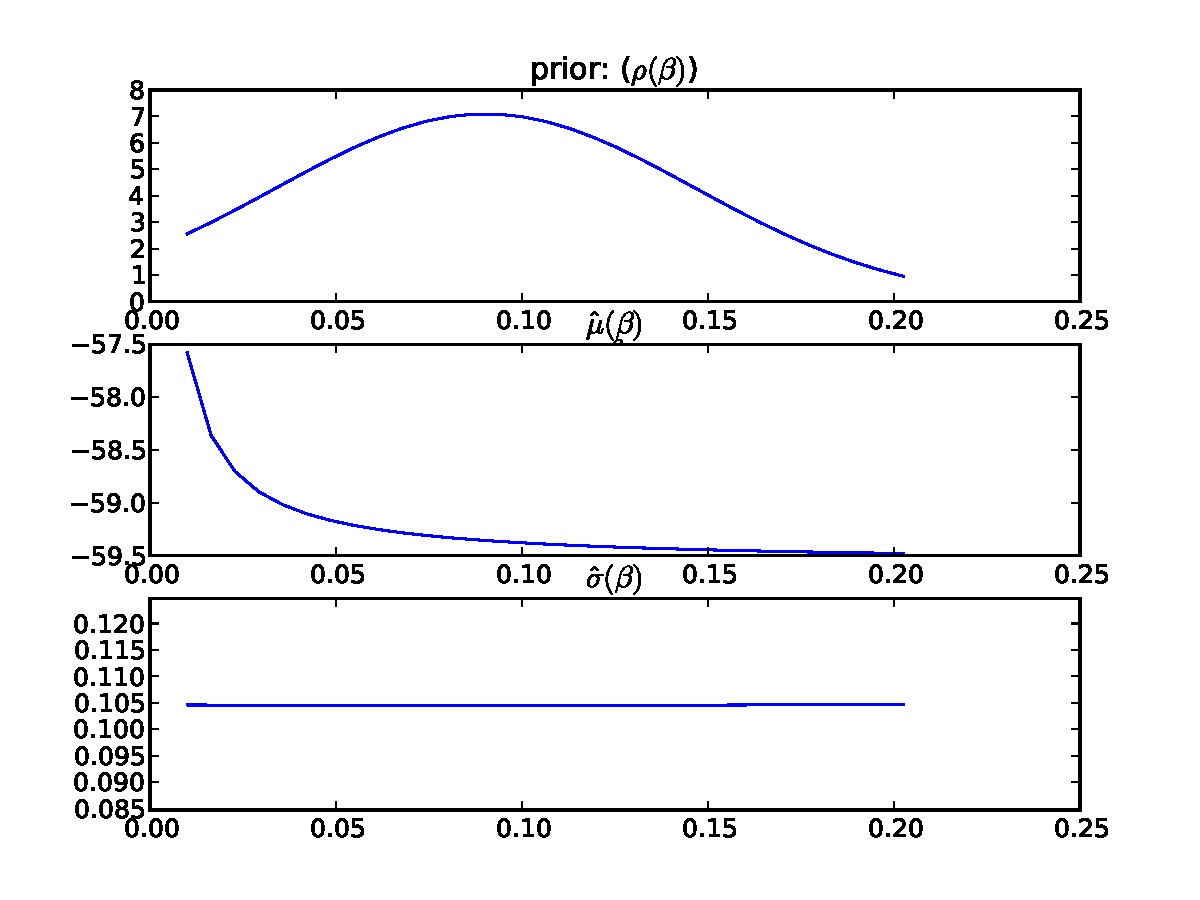
\includegraphics[width=0.48\textwidth]{Figs/MI/prior_example.pdf}
}
\subfloat[underlying $X$ path]
{
\label{fig:prior_path}
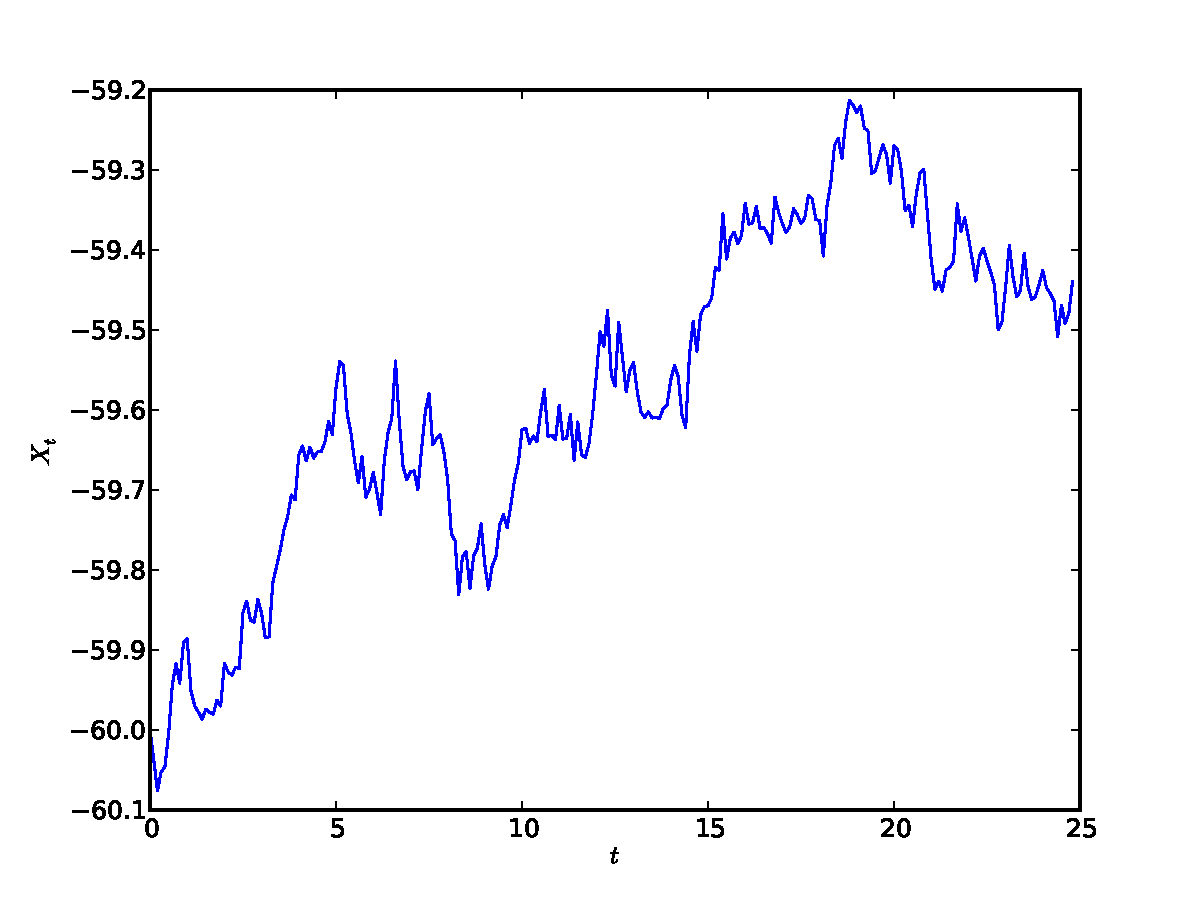
\includegraphics[width=0.48\textwidth]
{Figs/MI/prior_example_path.pdf}
}
\caption[labelInTOC]{An example of a path, a prior over $\b$ built based on
the path and the resulting functional relations between $\b$, $\m$ and $\s$,
which are from \cref{eq:mu_root,eq:sigma_root}. The prior for $\b$ and the
resulting $\m,\s$ are obtained using the path in (b)}
\label{fig:prior_mu_sigma}
\end{center}
\end{figure}
At this point we might start to think a normal prior for an a priori positive
random variable, like $\b$, is a bad idea, especially if we are near zero and the std.
dev. of the $\b$ belief distribution is non-negligible. Perhaps, we should use
a log-normal prior or a gamma distribution \ldots


Now let's calculate the integral of the likelihood wrt.\ the prior for a fixed
$x$, ie. the marginal forward distribution of $x$. $$ p(x) = \int_\Theta
L(x|\th;\a)\cdot \rho(\th) \intd{\th} $$ This is also the normalizing constant
in bayes rule. We will use a forward horizon of  $\Delta_f = 5$ (ms) (Recall the
data used to generate the prior distributions had $\Delta = 0.1$ and has length
$T = 50$ ms). $p(x)$ is shown in \cref{fig:marginal_px}. Essentially,
\cref{fig:marginal_px} is telling us that the current value of $x$ is lower than
the estimate for the long-term mean, all things considered. Our current
estimates for $\b, \m, \s$ are letting us believe that it should move up
towards approximately $59.5$ provided that we continue with the
current value of $\a=0$. 

The two opposing proposed values for $\a = \pm 0.25$ result in much
more spread distributions for $X_{t+\Delta_f}$. In particular, one might argue that
$\a=-0.25$ is most informative, since the forward distribution has the most
spread. (if we intuitively equate spread with information). This is consistent
with the notion that the most informative experiments are the ones that lead $X$
furthest from its current equilibrium (given $\a=0$). In this case the negative
is better than positive, since the current value of $X_t$ is already negative in
relation to the current equilibrium. Basically this is consistent with the
following selection mechanism of $\a$: If $X_t > \m$ choose $\amax$ otherwise
if $X_t < \m$ chose $\amin$. This is illustrated in
\cref{fig:marginal_px_shifted}, where we artificially move the value of $X_t$ to
the right of the (current) equilibrium, which makes the forward distribution
arising from $\a=0.25$ more informative (higher spread), then the one with
$\a=-0.25$.

\begin{figure}[htp]
\begin{center}
\subfloat[Left of equilibrium]{
  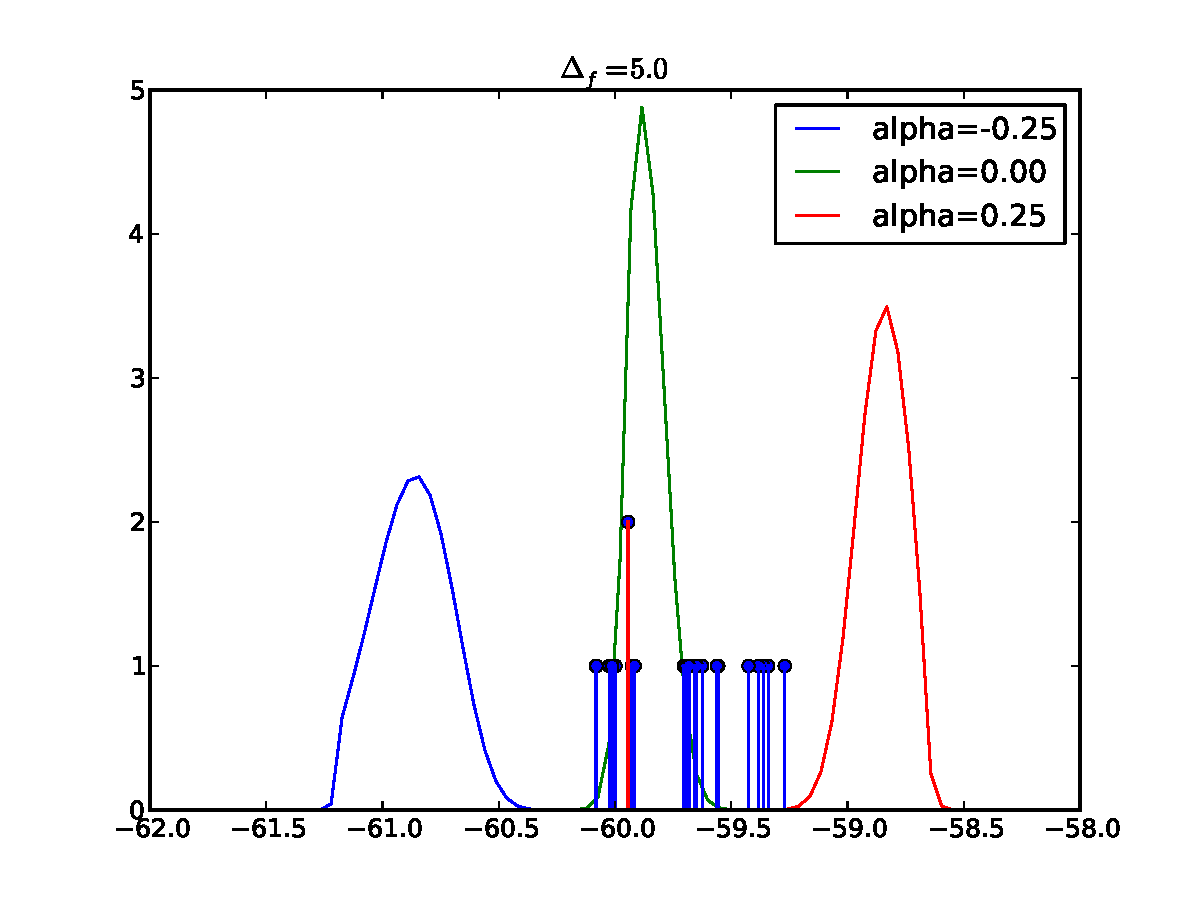
\includegraphics[width=.5\textwidth]{Figs/MI/x_marginal_example.pdf}
  \label{fig:marginal_px}
}
\subfloat[Right of equilibrium]{
  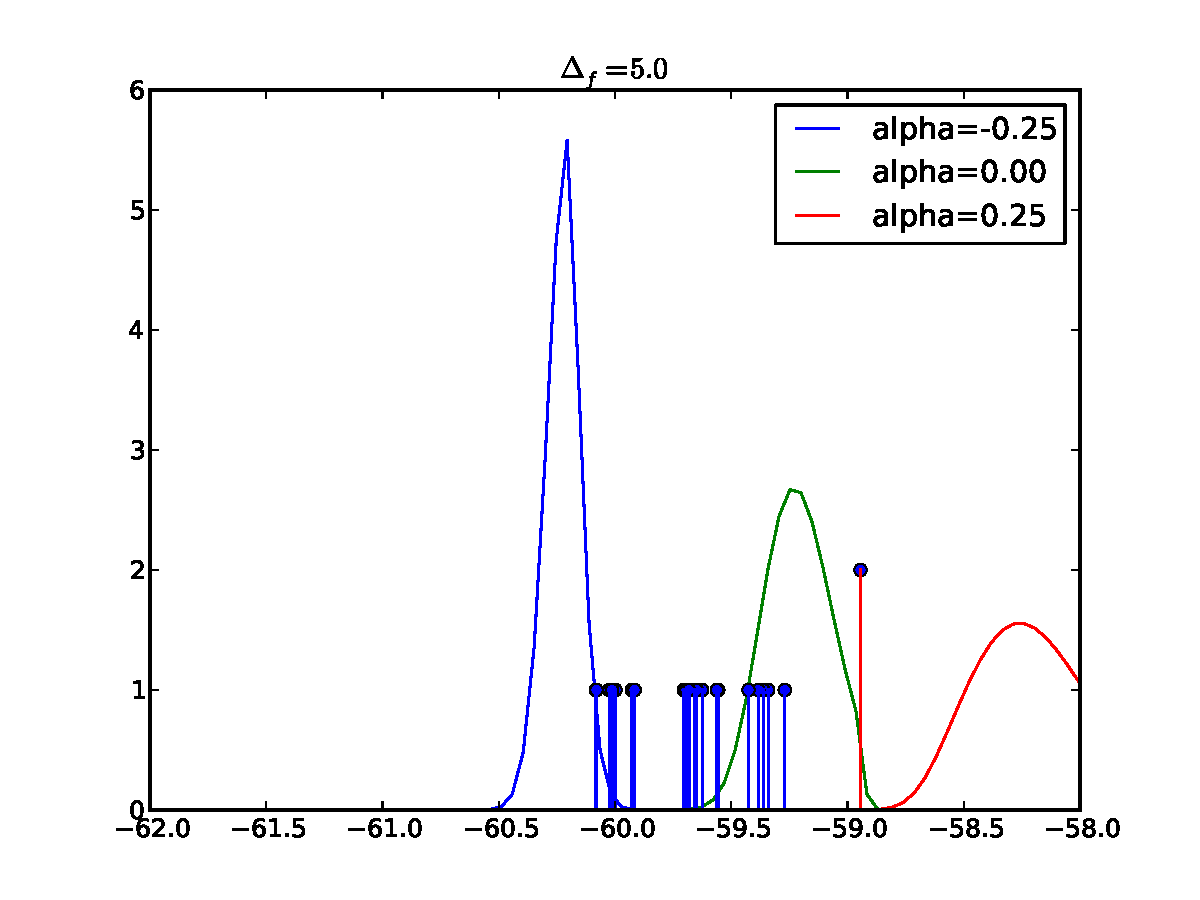
\includegraphics[width=.5\textwidth]{Figs/MI/x_marginal_example_x0_shifted_right.pdf}
    \label{fig:marginal_px_shifted}
  }
  \caption[labelInTOC]{
  Marginal of $x$ (normalizing constant), the tall red stem
  is the current value of $X_t$. This is the last observed value based on
  which we compute transition densities. The lower, blue stems are all the
  other data previously observed. The blue and red curves are forward densities
  given different applied forward values for $\a$. The green curve is the forward density given the hitherto used value of $\a=0$. It mostly coincides
  with the so-far observed data(the blue stems).
  In float (b) we artificially move the starting point to the right. Note that
  the green curves in a), b) are not the same, since they depend on the value
  of $X_t$ as well as the observed data ($X_t$ is different in the two
  panels, but all other data points, the blue stems, are the same)}
\end{center}
\end{figure}

Let us verify this intuition formally, by calculating $I(\a)$, for $\a =[-0.25 , 0, 0.25]$.

Aside: Unfortunately, naively calculating the double integral (in Python using
'quad' or 'romberg') is not numerically efficient. Calculating $I(\a)$ for a
single $\a$ takes on the order of 10 secs, once you relax the quadrature
tolerances without incurring any significant error\ldots Since we are dealing
with Gaussian-type integrals, a Gauss-Hermite Integration scheme might be very
effective, but we will leave that for now.

Crushing through the integration with brute force we get the result
in \cref{tab:MI_3alphas_basic_quad}.
\begin{table}
\begin{centering}
\begin{tabular}{cc}
$\a$& $I(\a)$ \\
-0.25  &
 0.688 
\\
0.00 &
   0.100 
\\
   0.25 &
   0.419 
\end{tabular}
\caption{values for the mutual information, $I(\a)$, for various values of
$\a$, starting from the value of $X_t$, (the red stem in
\cref{fig:marginal_px})}
\label{tab:MI_3alphas_basic_quad}
\end{centering}
\end{table}
We have used the same starting (current) value of $X_t$ to form the forward
likelihoods as in \cref{fig:marginal_px} and indeed we get the result.
$$I(-0.25) >I (.25) > I(.0)$$
which is consistent with our expectations after calculating the corresponding
$p(x)|\a$ in \cref{fig:marginal_px}. This basically says that it should be most
informative to stimulate down ($\a<0$), and it should be least informative to
do nothing $\a=0$.

 \subsection{Follow-up Estimation}
 Let's now see what that means in practice. Pretend that we have done the
 analysis instantaneously and let the process unroll further from $X_t$ for
some time. Then we will check if there is any advantage to
 using the mutually most informative $\a$, i.e.\ $\a = \argmax I(\a)$.
First we generate 10 forward trajectories of duration 2$\Delta_f = 10$ (ms).
They are shown in \cref{fig:perturbed_trajectories}. 
\begin{figure}[htp]
\begin{center}
  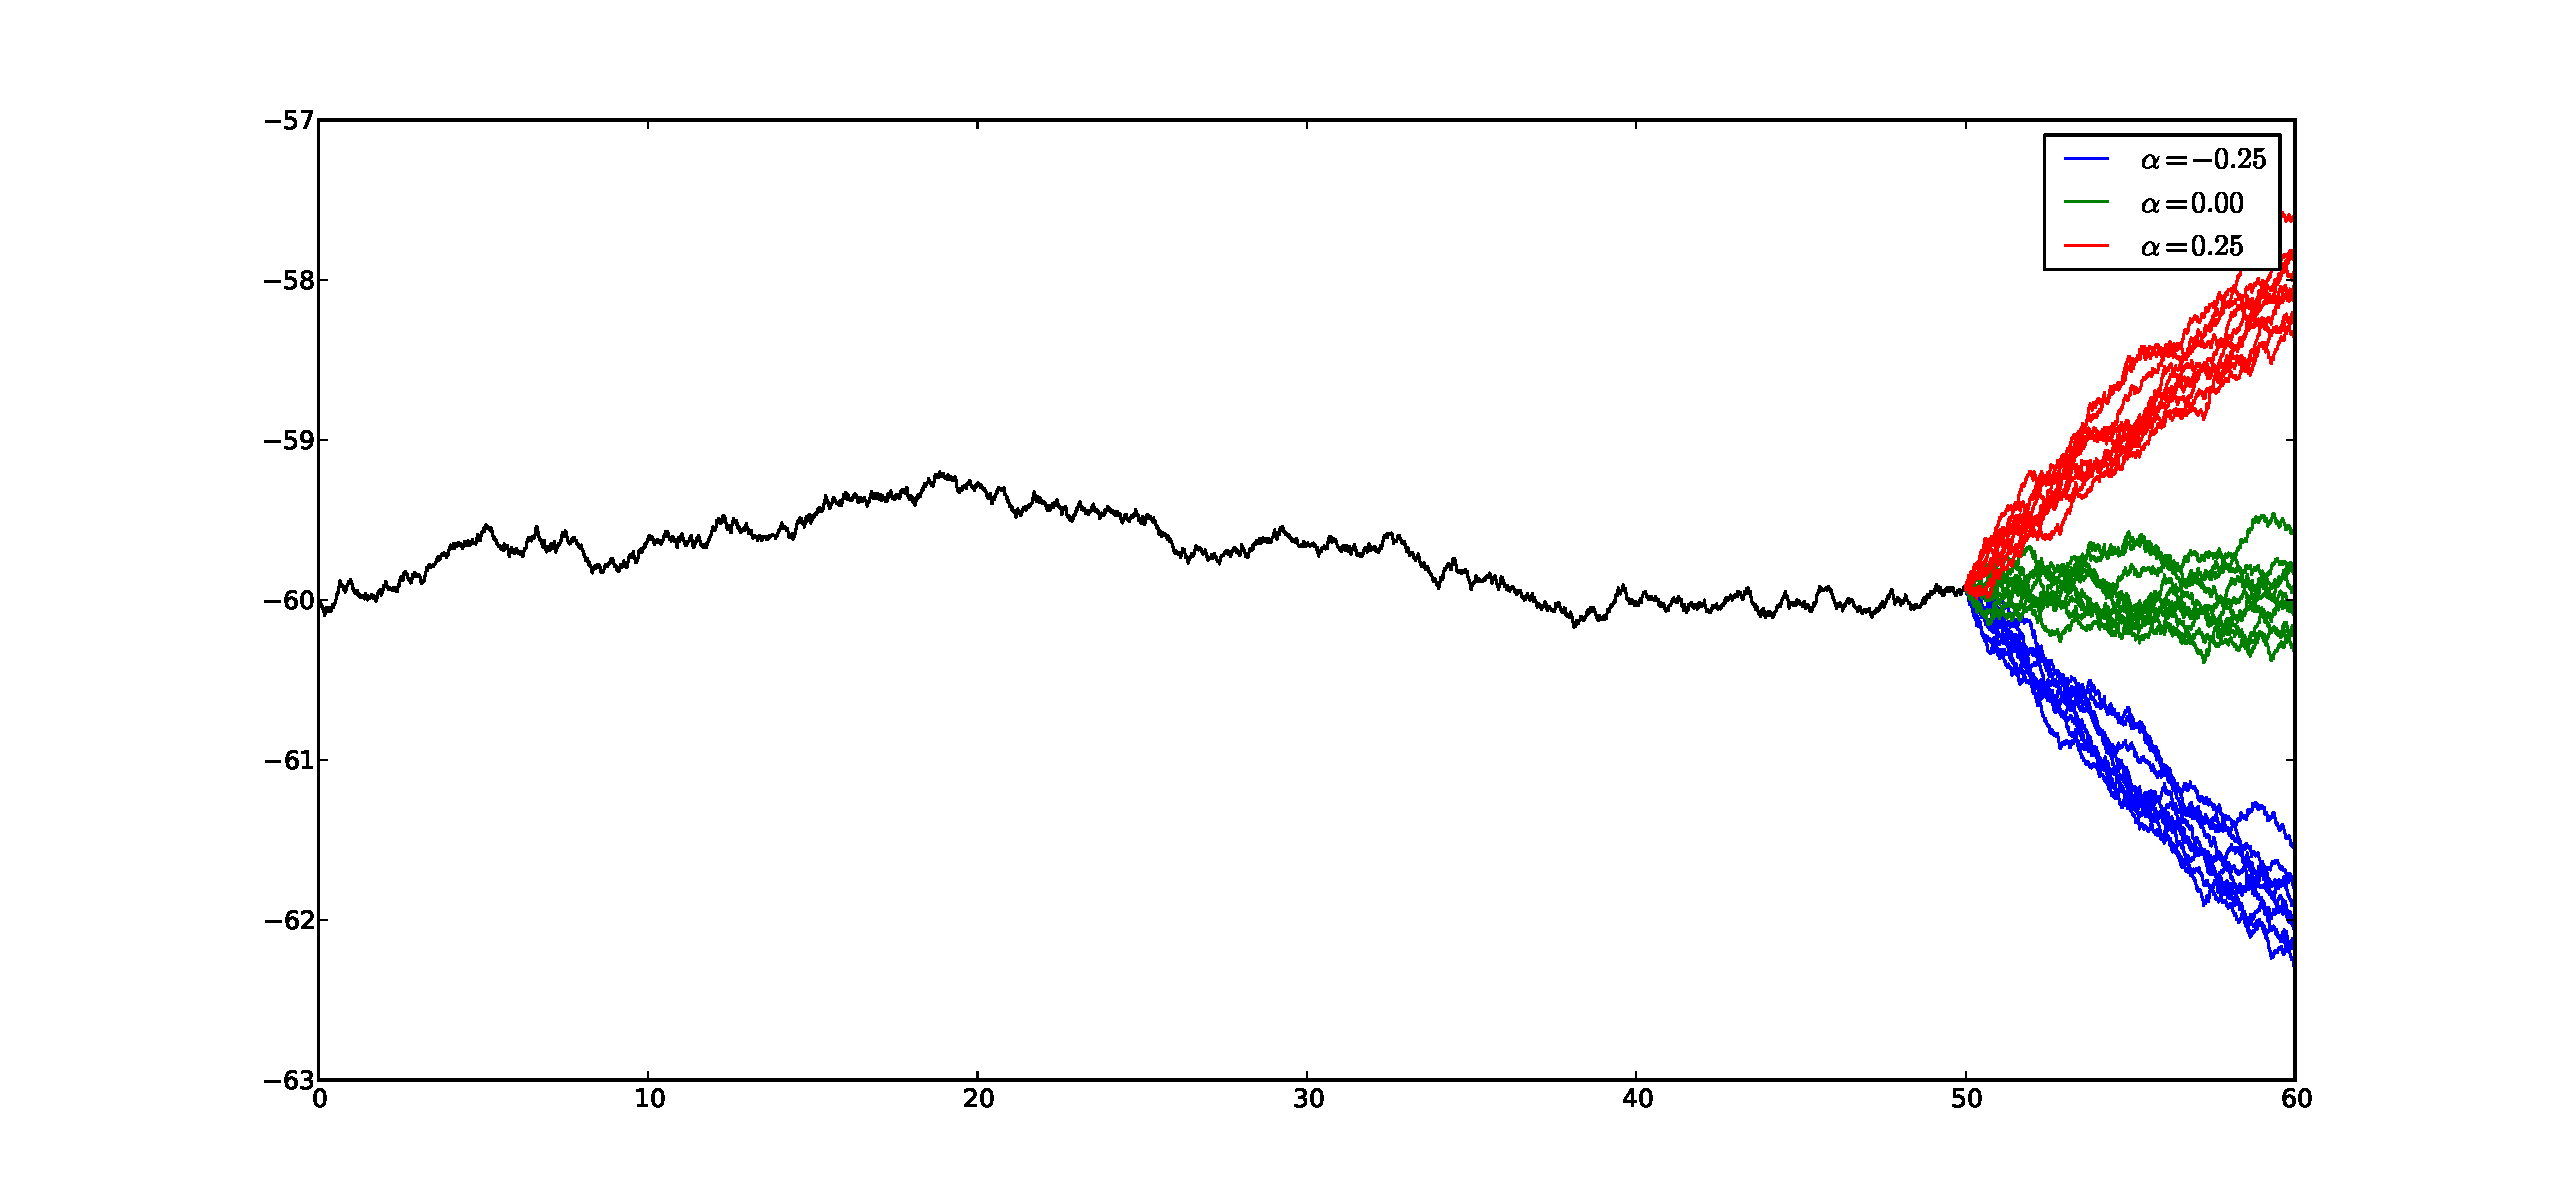
\includegraphics[width=1\textwidth]{Figs/MIML/forward_sims.pdf}
  \caption[labelInTOC]{Different Trajectories perturbed by different values of
  $\a$ after the MI calculation}
  \label{fig:perturbed_trajectories}
\end{center}
\end{figure}
% 
Now what we would like to see is that the estimates corresponding to $\a=-.25$
are 'better' than the ones corresponding to $\a=.25$ and that they are much
better than the ones corresponding to $\a=.0$.

Let's see: The resulting estimates for the 10 trajectories are shown in
\cref{fig:perturbed_estimates}. Well, what do you know, visually, it is clear
that indeed $\a=-.25$ is  'better' than $\a=.25$, which in turn is better than $\a=.0$.
\begin{figure}
\begin{center}
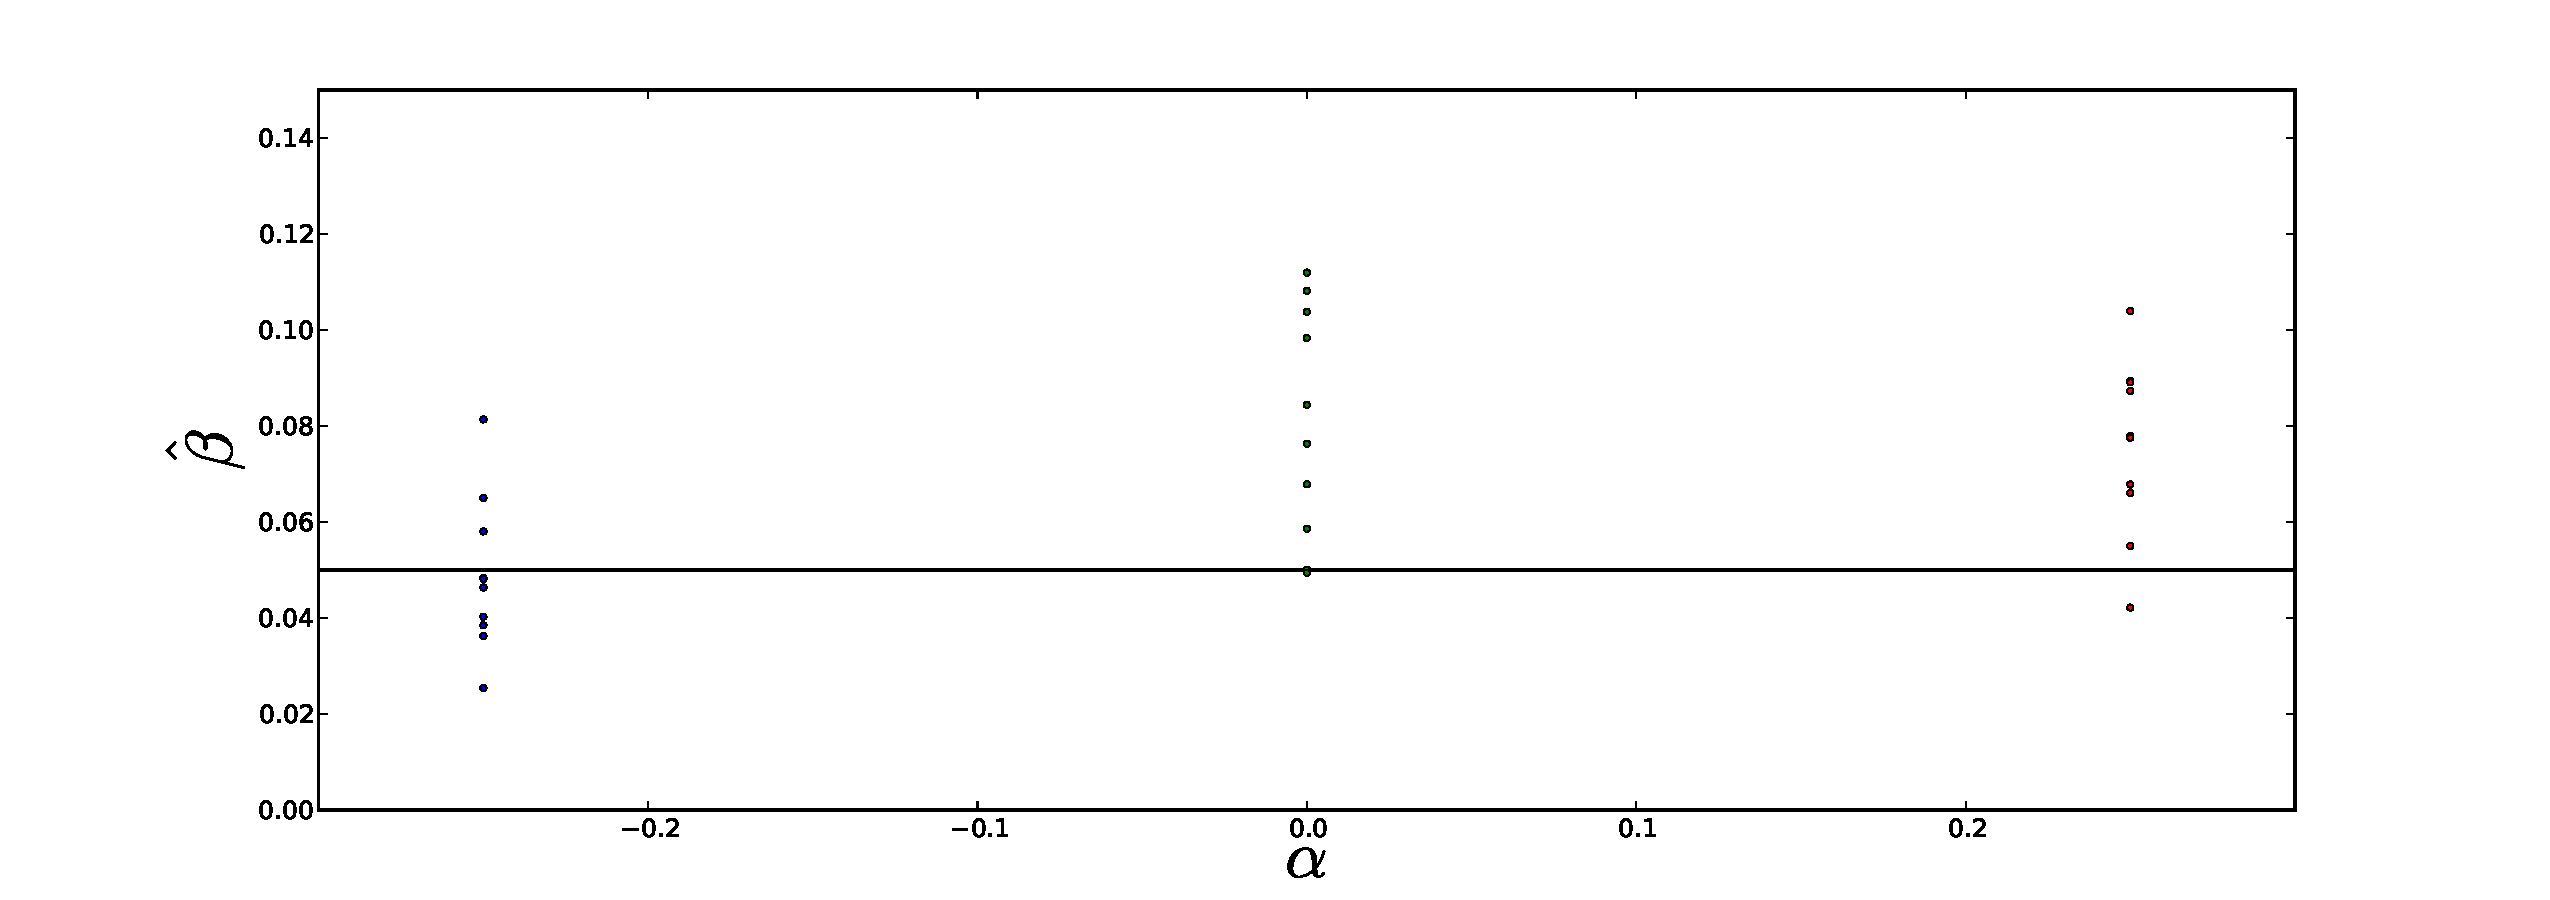
\includegraphics[width=1\textwidth]{Figs/MIML/perturbed_estimates.pdf}
\caption[]{The estimates for $\b$ given the three perturbed
trajectories (one is actually un-perturbed ($\a=.0$)). The solid black line
indicates the true value of $\b$}
\label{fig:perturbed_estimates}
\end{center}
\end{figure}

\subsection{Bang-Bang?}
We expect that it is actually best to apply maximum inhibition or maximum
excitation. That is we expect that $I(\a_2) > I(\a_1)$ for $|\a_2| > |\a_1|$. We
verify this in \cref{tab:MI_bang_bang_alphas}, where we see the general tendency
that bigger is more informative than smaller and negative is more informative
than positive.
\begin{table}
\begin{centering}
\begin{tabular}{cc}
$\a$& $I(\a)$ \\
-2&  2.31 \\
-1.00 & 1.714 \\
-0.50 & 1.182 \\
0.50 & 0.885 \\
1.00 & 1.563 \\
2.00 &  2.20 \\
\end{tabular}
\caption{values of MI}
\label{tab:MI_bang_bang_alphas}
\end{centering}
\end{table}
\Cref{tab:MI_bang_bang_alphas} and our intuition suggest then that the choice
for which is always between the two extremes st.\ $\a_{\textrm{most
informative}} \in \{\amin, \amax\}$.

Now we wonder what happens to the calculated value of $I$ as we move $\Delta_f$,
see \cref{fig:MI_delta_f_variation}. Now this is interesting. As $\Delta_f$
increases, we have a raise in the mutual information. Intuitively this is
obvious, since bigger $\Delta_f$ means more data. However, recall that we are
only considering the information contained in the final value (at $t=\Delta_f$).
That is also why $I$ levels off eventually, if we were considering the full path
and not just the final value, then it should continue increasing monotonically,
although perhaps with a decreasing slope. However! It is also clear that while
in the current context and for the current example at this time, inhibition is
best $I(-) > I(+)$. At some point in the future excitation will be better! That
is as the $X$ variable settles into its new, lower, equilibrium, $I(+) > I(-)$.

The question becomes how to formulate this problem as to decide on when to
switch. 
%\usepackage{graphics} is needed for \includegraphics
\begin{figure}[htp]
\begin{center}
  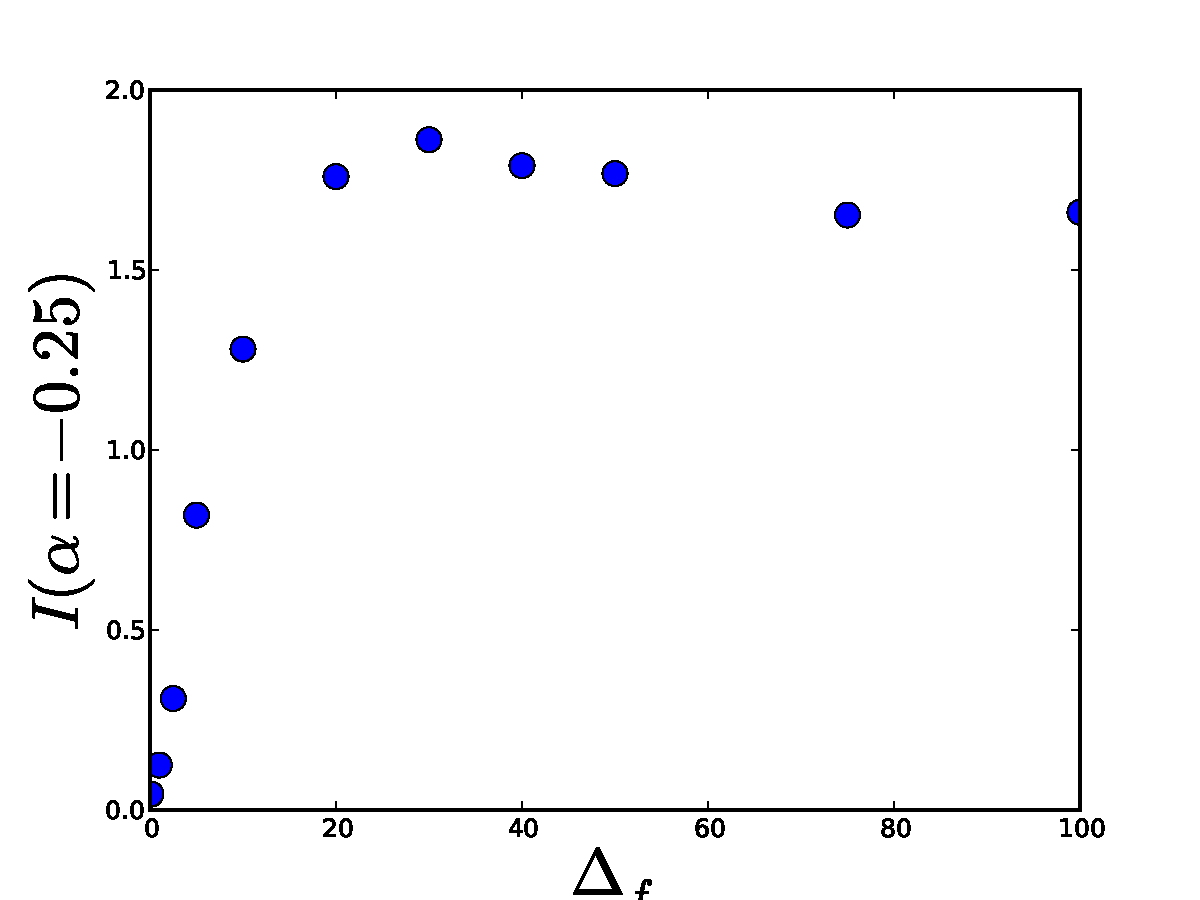
\includegraphics[width=1\textwidth]{Figs/MI/forward_deltas_vs_MIs.pdf}
\caption{values of MI while varying $\Delta_f$. Note that the right-most value
is a little iffy, as the integration routines warn about possible problems with
the various integrals}
	\label{fig:MI_delta_f_variation}
\end{center}
\end{figure} 
Let me explain why, potentially, this is an interesting problem, what is a
possible solution and why that solution is possibly very difficult to enact:

\subsection{Optimal Switching for Optimal Design}
Let us recap where (we think) we are:
There is an observed OU process $X_t$. We estimate it on the fly and have
estimates for $\b, \m, \s$ or more precisely we have a distribution for $\b$ and
a one-to-one relation between $\b$ and $\m,\s$. 

We have a control of $\a$ with which we can stimulate $X$. We want to use $\a$
to improve the observations of $\b, \m, \s$. We use the Mutual Information
criterion, $I(\a)$ to select $\a$. From the structure of the OU process, it is
conjectured and empirically observed that the bigger in magnitude $\a$ the more
informative it will be. Thus, in the absence of an energy cost, we are left only
to select between the two extreme values of $\a$, $[\amin, \amax]$, which
we can assume to be just $[\pm \amax]$ for some $\amax>0$. Thus at any time, $t$,
we can calculate $I(\amin), I(\amax)$ and choose the $\a$ associated with the larger $I$.

However, in a sense this is greedy and thus not necessarily optimal.

Here is a simple way to think about it:

Imagine that $\amin, \amax$ correspond to two equilibria
$\xmin, \xmax$. Our intuition is that there is a mid-point $\xmid$ between
$\xmin, \xmax$ st. if $X_t < \xmid$, we should apply $\amax$ and conversely. 
It is now clear that this can easily result in chattering - being below $\xmid$
we stimulate which sends us above $\xmid$ and then we inhibit, since above
$\xmid$ it is most informative to inhibit and so on. 

When you add the noise, it is hard to see if that is even a better idea than
doing nothing. 

Of course, things are not so simple as the distribution on the parameters,
$\rho$ may make $\xmid$ itself move as $\rho$  shifts and shrinks, but let's
ignore that for now. 

At this point it becomes clear that we need a way to choose the switching time
to switch between  $\amax, \amin$ using something more sophisticated than just
the instantaneous value of $I(\a)$. This is related to the problem of
how to choose the observation time $\Delta_f$ in the formulation of $I(\a)$. 

Basically we need to select what we are going to do now in part based on what we
can do later. And that is Dynamic Optimization!

The main difference here from standard Dynamic Optimization is
that our state is not so much the value of $X_t$ but the value of $\hat \b_t,
\hat \m_t, \hat \s_t$, the estimates at time $t$. Once we realize this, we also
realize our main challenge - the updates for $\b, \m, \s$ using the ML
formulas are non-Markovian! That is we look back on all the old
data when taking the new data into account to form $\hat \b_t, \hat \m_t, \hat
\s_t$. 

We could consider further one of two things
\begin{enumerate} 
  \item come up with a heuristic way of choosing $\Delta_f$ before which to
  consider switching (if $\Delta_f$ is large enough, we will always switch (I
  think))
  \item Come up with an incremental form for updating $\b$
\end{enumerate}

In the next section we do NEITHER:) Instead we consider the Optimal Design
problem, ie. the selection of $\a(\cdot)$ from the point-of-view of
Stochastic Optimal Control Theory.



\section{Finding the optimal design $\a(\cdot)$ using Stochastic
Optimal Control}

In principle now, we have a criterion, the mutual information in
\cref{eq:mutual_info_with_likelihood}, using which to select the most
informative perturbation $\a(\cdot)$. Intutitively, the 'optimal'  $\a(t)$
depends on the up-to $t$ realization of $X_s ; s\leq t$. This is clearly a
problem from optimal stochastic control. However, the objective in
\cref{eq:mutual_info_with_likelihood} is not in the form needed to apply dynamic
programing (or the maximum principle for that matter). The multi-dimensional
integral in $X$ makes things 'too' complicated.

On the other hand, a possible simplification is to take the mutual information
criterion in \cref{eq:mutual_info_with_likelihood} using the single observation
likelihood in \cref{eq:paramter_likelihood_single_observation} and just
integrate it over time.
\begin{equation}
J(\a)  = \int_\th \int_0^T\int_{X_t}
 \log\left(\frac{f(x,t|\th ; \a(\cdot) )}
 			{\int_\th f(x,t|\th; \a(\cdot)) \rho(\th)\intd{\th}}\right) 
 f(x,t|\th; \a(\cdot)) \cdot \rho(\th) \intd{x}\intd{t}\intd{\th}
\label{eq:mutual_info_time_integrated}
\end{equation}
where the $dx$ integral has the same dimension as the dimension of the SDE not
the dimension of the SDE times the number of observations. I should repeat that
$J$ is NOT the mutual information between a realization of the process, $\{
X_t\}_0^T$ and the parameter set, $\th$. It is the time-integral of the
individual mutual informations between each $X_t$ at time $t$ and the parameter
set $\th$. 

The reason we would like to consider this simplification is that now
$J$ can be written as
\begin{equation}
J( \a) = \Exp_{\th} \Bigg[
\Exp_{X_t|\th; \a(\cdot)}
\left[ \int_0^T \log\left(\frac{f(X_t,t|\th; \a(\cdot))}
{\int_\th f(X_t,t|\th; \a(\cdot)) \rho(\th)\intd{\th}}\right) \intd{t} \right]
\Bigg] 
\label{eq:mutual_info_time_integrated_as_expectations}
\end{equation}
which almost has the classical form of a stochastic optimal control
problem, except for two non-standard features:
\begin{enumerate}
  \item We have an extra outer expectation, this is the integration wrt. to the
  parameter prior.
\item There is a forward-backward coupling in the determinations of the optimal
control, meaning we can't just back out, the optimal control with a backwards
solution to an HJB equation
\end{enumerate}
Of these two features, we discuss pt. 1 first.

\subsection{Stochastic Optimal Control with a Prior}
We would like to apply Dynamic Programing to the problem of maximizing
\cref{eq:mutual_info_time_integrated_as_expectations}. However
\cref{sec:DP_with_a_prior} shows why this is impossible (or at least why the
first thing one thinks of does not work).

Instead, in \cref{sec:MP_with_a_prior}, we use the Maximum Principle in order to
find the optimal $\a(\cdot)$.

\subsubsection{Dynamic Programing with a Prior}
\label{sec:DP_with_a_prior}

WARNING: THIS SECTION ULTIMATLY EXPLAINS WHY YOU \underline{CANNOT!} USE
\cref{eq:HJB_equation_with_prior}. I.E. WHY DYNAMIC PROGRAMING CANNOT! BE
USED TO FIND THE CONTROL, $\a(\cdot)$. 

\vskip 15pt

In order to apply Dynamic Programing, i.e. in order to set up an HJB PDE, let us
write our objective as:
\begin{equation}
J(x_0, 0; \a) = \Exp_\th \Bigg[ \Exp_{X_0^T|\th, \a} \bigg[ \int_0^T r(X_t|
\th)\intd{t} \bigg]\Bigg]
\label{eq:stochastic_objective_with_prior_generic} 
\end{equation}
where, in our case, the reward $r$ is the mutual information between $X_t$ and
$\th$ 
\begin{equation}
r(x|\th) = \log\left(\frac{f(x,t|\th; \a(\cdot))}
{\int_\th f(x,t|\th; \a(\cdot)) \rho(\th)}\right)
\label{eq:reward_funciont_mutual_information}
\end{equation}
But we can consider $r(\cdot)$ as a generic function of $X_t$.

Now we try to follow the standard dynamic programing approach to obtain an
HJB-type equation. 

Call $w$ the value function, i.e.\ the optimal reward-to-go.
\begin{equation}
w(x_t, t) = \sup_{\a(\cdot)} 
\Exp_\th \Bigg[ \Exp_{X_t^T|\th, \a} \bigg[ \int_t^T r(X_t| \th) \intd{t}
\bigg]\Bigg]
\label{eq:value_function_with_prior_defn}
\end{equation}
Or in particular, starting from $x_0$ at $t=0$ 
\begin{equation}
w(x_0, 0) = \sup_{\a(\cdot)} 
\Exp_\th \Bigg[ \Exp_{X_0^T|\th, \a} \bigg[ \int_0^T r(X_t| \th) \intd{t}
\bigg]\Bigg]
\end{equation} 

$$
\Exp_{X_0^T|\th, \a} [\cdot] 
$$
means the expectation over the full trajectory of $X$ from $0$ to $\T$, $X_0$
held fixed, while evolving under the parameter set $\th$ and the control
policy $\a$.
$$
\Exp_{\Delta X|\th, \a} [\cdot] 
$$
Is the expectation over the single point realization of $\Delta X = X(\Delta t)
= X_{\Delta t}$, again under a given parameter set and policy, $\th, \a$.

The Markovian nature of $X_t|\th$ implies that for $x_0$ fixed.
$$
\Exp_{X_0^T|\th, \a} [\cdot ] =
\Exp_{\Delta X|\th} \Big[ \Exp_{X_{\Delta t}^T|\th, \a} [ \cdot  | \Delta X ]
\Big] $$

With that we can start deriving an equation for $w$, starting from
\begin{align*}
w(x_0, 0) =& \sup_{\a(\cdot)} 
\Exp_\th \Bigg[ \Exp_{X_0^T|\th, \a} \bigg[ \int_0^T r(X_t| \th) \intd{t}
\bigg] \Bigg]
\\
=&  \sup_{\a(\cdot)} 
\Exp_\th \bigg[ r(x_0) \Delta t \bigg] + 
\Exp_\th \Bigg[ \Exp_{X_0^T|\th, \a} \bigg[ \int_{\Delta t}^T r(X_t| \th)
\intd{t} \bigg] \Bigg]
\end{align*}
All we've done so far is split the time integral into an incremental initial
part which is approximately equal to $r(x_0)\dt$ and the rest $\smallint_\dt^T$.
Now let's focus on the second term, $\Exp_\th \Big[ \Exp_{X_0^T|\th, \a} \big[ \int_{\Delta t}^T r(X_t| \th)
\intd{t} \big] \bigg]$ and condition on $x_0 + \Delta X$:
\begin{align*}
\Exp_\th \Bigg[ \Exp_{X_0^T|\th, \a} \bigg[ \int_{\Delta t}^T r(X_t| \th)
\intd{t} \bigg] \Bigg]
=&  
\Exp_\th \Bigg[ \Exp_{\Delta X |\th, \a} \Big[ \Exp_{X_{\dt}^T|\th, \a}
\int_\dt^T r(X_t| \th) \intd{t} | X_\dt \Big] \bigg] \Bigg]
\end{align*}

Now here is the main problem! We WOULD LIKE to say that
\begin{multline}
\Exp_\th \Bigg[ \Exp_{\Delta X |\th, \a} \Big[ \Exp_{X_{\dt}^T|\th, \a}
\int_\dt^T r(X_t| \th) \intd{t} | X_\dt \Big] \bigg] \Bigg] 
= \\
\Exp_\th \Bigg[ \Exp_{\Delta X |\th, \a} \Big[ 
\underbrace{\boldsymbol{\Exp_\th}}_{\uparrow\textrm{add this?} \uparrow} \Big[
\Exp_{X_{\dt}^T|\th, \a} \int_\dt^T r(X_t| \th) \intd{t} | X_\dt \Big]\Big]
\quad \bigg] \Bigg]
\label{eq:incremental_bellman_with_falsely_added_prior}
\end{multline}
Because then we could plug in $w(x_0 + \Delta X, \Delta t)$ in:
$$
\Exp_\th \Bigg[
\Exp_{X_{\dt}^T|\th, \a} \int_\dt^T r(X_t| \th) \intd{t} | X_\dt \Big]\Bigg] =
 w(x_0
+ \Delta X, \Delta t) $$
And then the rest rolls off easily to get the PDE:
\begin{equation}
\di_t w(x,t) + \sup_{\a(x,t)} \bigg\{  \Exp_\th \big[\Lstar_\th [w] +
r(x|\th)\big] \bigg\} = 0
\label{eq:HJB_equation_with_prior}
\end{equation}
Where $\Lstar_\th$ is the generator (backward Kolmogorov operator) corresponding
to the SDE \cref{eq:SDE_evolution} for fixed parameters, $\th$,
$$
\Lstar_\th[\cdot] = U(x,\a; \th) \di_x[\cdot] + D \di_x^2[\cdot]
$$

HOWEVER! Can we just put the extra
$\Exp_\th$ in \cref{eq:incremental_bellman_with_falsely_added_prior}? 

It comes down to what exactly is the meaning of the prior on
SDE parameters. Is it that:
\begin{enumerate}
  \item You choose $\th$ at each time-step (infinitesimally going to 0) let $X$
  evolve accordingly for an increment $dt$ and then choose $\th$ again.
  \\
  or
  \item You choose $\th$ at time $0$ and then let $X$ evolve accordingly to this
  once-and-for-all fixed $\th$
\end{enumerate}

If it is the former, then we can indeed add the extra expectation wrt.\ $\th$
in \cref{eq:incremental_bellman_with_falsely_added_prior} and then use
\cref{eq:HJB_equation_with_prior} to compute $w$. If it is the latter, then we
cannot.

HOWEVER! Assuming pt.1, i.e.\ that we re-choose $\th$ at each incremenent,
fundamentally violates the basic point of the parameter estimation.

Let me explain.

We suppose that the underlying process $X$ is governed by a single value of
$\th$, we just don't know which. We would like to observe the
trajectory of $X$ so as to determine which is the underlying value of $\th$, but
if we re-choose $\th$ at each time-increment of $X$'s evolution, then there is
NO single $\th$ and indeed the whole estimation problem is moot.

So adding the inner expectation wrt.\ $\th$ in
\cref{eq:incremental_bellman_with_falsely_added_prior} is wrong! And solving
\cref{eq:HJB_equation_with_prior} will not at all help in finding the maximally
informative stimulus $\a(\cdot)$.

More mundanely, I actually, computed the solution to
\cref{eq:HJB_equation_with_prior} for the Double-Well Potential and it gives
non-sense results (for $\a$ AND $w$\ldots)

We must try something else!


\subsubsection{Maximum Principle with a Prior}
\label{sec:MP_with_a_prior}
Let us go back to the original objective,
\cref{eq:mutual_info_time_integrated} or equivalently
\cref{eq:mutual_info_time_integrated_as_expectations}
$$
J(\a)  = \int_\th \int_0^T\int_X
 \log\left(\frac{f(x,t|\th ; \a(\cdot) )}
 			{\int_\th f(x,t|\th; \a(\cdot)) \rho(\th)\intd{\th}}\right) 
 f(x,t|\th; \a(\cdot)) \cdot \rho(\th) \intd{x}\intd{t}\intd{\th}
$$

$J$ then is a functional of a family of distributions $f(|\th)$ parametrized by
$\th$.

We will write this as:
$$
J(\a)  = \Exp_\th \left[ \int_0^T\int_{\O_X}
r(f(x,t|\th; \a(\cdot))) \cdot   
 f(x,t|\th; \a(\cdot)) \intd{x}\intd{t} \right]
$$ 

Then optimizing $J$ looks a lot like the a generic problem in optimizing over
PDEs with the added complexity of the outer expectation (the one wrt.\ $\th$).

We now attempt to set up a Pontryagin-Type equation for the optimal value of
$\a$: We start by augmenting the objective with the dynamics:
\begin{equation}
J =  \Exp_\th
\left[ \int_0^T\int_{\O_X} r(f) \cdot f - p \cdot (\di_t f - \L_{\th;\a}[f])
\intd{x}\intd{t}\right] 
\label{eq:objective_augmented}
\end{equation} 
where $p =  p(x,t|\th; \a(\cdot))$ is the adjoint co-state and $\di_t f -
\L_{\th;\a}[f]$ is the Fokker-Planck equation,
\cref{eq:fokker_planck_forward_density}.

What we are going to do is calculate the differential of $J$ wrt.\ $\a(\cdot)$
and then use this in a gradient ascent procedure. First what we would like to do
is transfer all the differentials from $f$ to $p$. That is we will integrate $p
\cdot (\di_t f - \L[f])$ by parts so that only $f$ appears in the expression
without any of its derivatives. This is a standard exercise, we show it in
detail:
\begin{align*}
&-\int_0^T \int_{\O_X} p \cdot (\di_t f - \L[f]) \intd{x} \intd{s}=
\\
=&-\int_0^T \int_{\O_X} p \cdot 
(\di_t f_0 - D \cdot \di_x^2 f + \di_x [U \cdot f]
\intd{x} \intd{t} \quad \textrm{// what is }\L
\\
=&
 \int_0^T\int_{\O_X} \di_t p  f \intd{x} \intd{t} +
  \int_{\O_X} p f\intd{x}  \Big|^{T}_{t=0} \quad \textrm{// the time-derivative pieces }
  \\
  &+ \int_0^T \int_{\O_X}
	    (D \di^2_x p + U \di_x p)\cdot f 
	  \intd{t}\intd{x}  \textrm{// the space-derivative pieces }
	  \\
	  &+ \int_0^T 
	   \Big( p U f - p D \di_xf + \di_x p D f \Big|_{x=\xmin}^{\xmax} 
	  \intd{t}
	   \textrm{// the BC terms in 1-d}
\end{align*}

Thus the terminal and boundary conditions of $p$ are chosen given those of $f$
and the objective $J$. Since there are no boundary or terminal terms
contributing to our $J$, only the boundary conditions for $f$ impact the
choice of boundary conditions for $p$. In particular the following has to be
true:
\begin{align*}
pf&\Big|_{t=T}  = 0 & \textrm{Null TCs} \\
p U f - p D \di_xf + \di_x p D f &\Big|_{x=\xmin, \xmax} = 0 & \textrm{Null BCs}
\end{align*}

This usually implies that $p(T) \equiv 0$, since there are usually no a priori
restrictions on $f$ at the terminal time. For the boundary terms, 
if the forward density has reflecting boundaries such that:
$$
U f - D\di_x f\Big|_{x=\xmin, \xmax}  = 0
$$
then the BC terms for the adjoint are just the simple Neumann BCs:
$$
\di_x p \Big|_{x=\xmin, \xmax} = 0
$$

Once this integration-by-parts is done and the appropriate BCs applied, we
can return to the augmented objective, \cref{eq:objective_augmented} which now
looks like:
\begin{equation}
J =  \Exp_\th
\left[ \int_0^T\int_{\O_X} \log\left(\frac{f_\th}
 					{\int_\th f_\th \cdot \rho(\th)\intd{\th}}\right) 
 			 \cdot f_\th 
 			 + 
 			 (\di_t p_\th + \Lstar_{\th;\a}[p_\th] ) \cdot f_\th
\intd{x}
\intd{t} \right]
\label{eq:objective_augmented_adjoined}
\end{equation}
with $\Lstar$ the adjoint operator to $\L$.

The next step is to take the differential of $J$ wrt.\ the control
$\a(x,t)$

% Conceptually this is best imagined for a one-dimensional $X$. Basically,
% $\a(x,t)$ is like a sheet in $x-t$ space and the differential of $J$ is telling
% us how to move this sheet at any given point in order to improve the overall
% $J$. 

In order to make things simpler, we will write the integral wrt.\
$\th$ as a sum, i.e.:
$$
\int_\Theta f(\th) \rho(\th) \intd{\th} = \Exp_\th [f(\th) ] = 
\sum_\th w_\th (f(\th))
$$ where the weights $w_\th$ approximate the density $\rho(\th)$.
If one assumes a discrete prior this is just a different way of writing the
integral, if the prior is assumed continuous, then this is an approximation.
Then $J$ reads like:

$$
J =  \Exp_\th
\left[ \int_0^T\int_{\O_X} \log\left(f_\th\right)\cdot \ft - 
\log(\sum_\th \wt \ft) \cdot f_\th 
 			 + 
 			 (\di_t p_\th + \Lstar_{\th;\a} [p_\th] ) \cdot f_\th
\intd{x}
\intd{t} \right]
$$
and its differential wrt.\ $\a$ for given $x,t$ is:
\begin{align*}
\delta J|_{x,t} =& \sum_\th \Big[
\frac{\dft}{\ft} \cdot \ft - \frac{  w_\th \dft }{\sum_\th w_\th\ft}\cdot \ft 
+ \log\left(\frac{f_\th} {\sum_\th \wt \ft }\right) \cdot \dft  
\\&
+  (\di_t p_\th + \Lstar_{\th;\a} p_\th ) \cdot \dft
+ \delta \a \cdot (\di_x \pt \cdot \ft)
\Big]
\\
=& \sum_\th \Bigg[\Big(
1 - \frac{  w_\th \ft }{\sum_\th w_\th\ft} 
+ \log\left(\frac{f_\th} {\sum_\th \wt \ft }\right)   
+  (\di_t p_\th + \Lstar_{\th;\a} p_\th )
\Big)  \cdot \dft 
\\
&+ \delta \a \cdot (\di_x \pt \cdot \ft)
\Big]
\end{align*}
Now we need to knock out the $\dft$ terms so that we are left with only $\delta
\a$ terms. Thus we set the coeffiecent of $\dft$ to zero, which completes the 
evolution equation for a given $p_\th$
\begin{equation}
-\di_t \pt = 
\Lstar_{\th;\a} [p_\th] +  
1 - \frac{  w_\th \ft }{\sum_\th w_\th\ft} 
+ \log\left(\frac{f_\th} {\sum_\th \wt \ft }\right)   
\end{equation}
And once $\pt, \ft$ are solved for, the differential wrt.\ $\a$ comes
out to:
\begin{equation}
\frac {\delta J}{\delta \a} \Big|_{x,t} = \sum_\th (\di_x \pt \cdot \ft)
\label{eq:differential_objective_wrt_control_final}
\end{equation}
\Cref{eq:differential_objective_wrt_control_final} forms the key ingredient
in our gradient search for the most informative perturbation $\a^*(x,t) =
\argmax J(\a)$.


\subsubsection{Stationary Maximum Principle with a Prior}
\label{sec:StatMP_with_a_prior}
Let us now consider a variation on the Maximum Principle approach, when we just
maximize the Mutual Information between the stationary distribution and the
prior.

This amounts to changing the objective in
\cref{eq:mutual_info_time_integrated} to  
$$
J(\a)  = \int_\th \int_X
 \log\left(\frac{f(x|\th ; \a(\cdot) )}
 			{\int_\th f(x|\th; \a(\cdot)) \rho(\th)\intd{\th}}\right) 
 f(x|\th; \a(\cdot)) \cdot \rho(\th) \intd{x}\intd{\th}
$$

In effect this is a simplified version of \cref{sec:MP_with_a_prior}, where we
ignore the time evolution of $f$ and focus on its long-term equilibrium.

The calculations are very similar with the exception of $\di_t f = 0$. We start
by augmenting the objective with the dynamics:
\begin{equation}
J =  \Exp_\th
\left[ \int_{\O_X} r(f) \cdot f + p \cdot \L_{\th;\a}[f]
\intd{x}\right] 
\label{eq:objective_stat_augmented}
\end{equation} 
where $p =  p(x|\th; \a(\cdot))$ is the statinoary adjoint co-state and 
$\L_{\th;\a}[f]$ is the right hand of the Fokker-Planck equation,
\cref{eq:fokker_planck_forward_density}.

What we are going to do is calculate the differential of $J$ wrt.\ $\a(\cdot)$
and then use this in a gradient ascent procedure. First what we would like to do
is transfer all the differentials from $f$ to $p$. That is we will integrate $p
\cdot (\L[f])$ by parts so that only $f$ appears in the expression
without any of its derivatives. This is done exactly as before:
\begin{align*}
& \int_{\O_X} p \cdot (\L[f]) \intd{x}=
\\
=& \int_{\O_X}
	    (\Lstar[p])\cdot f 
	 \intd{x}  \textrm{// the space-derivative pieces }
	  \\
	  &+ \int_0^T 
	   \Big( p U f - p D \di_xf + \di_x p D f \Big|_{x=\xmin}^{\xmax} 
	   \textrm{// the BC terms in 1-d}
\end{align*}
Thus we keep the BCs as in the time-dependent section
\cref{sec:MP_with_a_prior}, and ditch the TCs:
\begin{align*}
p U f - p D \di_xf + \di_x p D f &\Big|_{x=\xmin, \xmax} = 0 & \textrm{Null BCs}
\end{align*}
Once this integration-by-parts is done and the appropriate BCs applied, we
can return to the augmented objective, \cref{eq:objective_augmented} which now
looks like:
\begin{equation}
J =  \Exp_\th
\left[ \int_{\O_X} \log\left(\frac{f_\th}
 					{\int_\th f_\th \cdot \rho(\th)\intd{\th}}\right) 
 			 \cdot f_\th 
 			 + 
 			 (\Lstar_{\th;\a}[p_\th] ) \cdot f_\th
\intd{x}
\right]
\label{eq:objective_stat_augmented_adjoined}
\end{equation}

Taking the differential of $J$ wrt.\ the control $\a(x,t)$ gives
\begin{align*}
\delta J|_{x} =&
\sum_\th \Bigg[\Big(
1 - \frac{  w_\th \ft }{\sum_\th w_\th\ft} 
+ \log\left(\frac{f_\th} {\sum_\th \wt \ft }\right)   
+  \Lstar_{\th;\a} p_\th
\Big)  \cdot \dft 
\\
&+ \delta \a \cdot (\di_x \pt \cdot \ft)
\Big]
\end{align*}
This gives us the differential equation for the adjoint $p$
\begin{equation}
0 = 
\Lstar_{\th;\a} [p_\th] +  
1 - \frac{  w_\th \ft }{\sum_\th w_\th\ft} 
+ \log\left(\frac{f_\th} {\sum_\th \wt \ft }\right)   
\end{equation}
And once $\pt, \ft$ are solved for, the differential wrt.\ $\a$ comes
out to:
\begin{equation}
\frac {\delta J}{\delta \a} \Big|_{x} = \sum_\th (\di_x \pt \cdot \ft)
\label{eq:differential_objective_stationary_wrt_control_final}
\end{equation}
\Cref{eq:differential_objective_stationary_wrt_control_final} forms the key ingredient
in our gradient search for the most informative {\sl stationary} perturbation
$\a^*(x) = \argmax J(\a)$. It is exactly the same as
\cref{eq:differential_objective_wrt_control_final} and it is imagine that
\Cref{eq:differential_objective_stationary_wrt_control_final} can be derived
from \cref{eq:differential_objective_wrt_control_final} without going to all
the trouble above\ldots
 

\section{Illustrative Example - Double Well Potential}
\subsection{Maximum Principle Approach - Time-Dependent Case}
\label{sec:MP_Doublewell_TimeDependent}
We now follow up the theoretical developments from \cref{sec:MP_with_a_prior}
with a concrete example.

Our first test problem will be the problem on estimating the double-well
potential barrier height as in Sec. 4 of the latest draft of Hooper et al.
\cite{Lin} on arXiv. (From June 7th, 2013). We shall use exactly the same parameter values
etc. as in sec. 4 in \cite{Lin}.

We would now like to compute the forward density and the adjoint functions
$\{\ft, \pt\}$ for the double-well problem.

Let's explicitly state the evolution equations for $\ft,\pt$
\begin{equation}
\begin{gathered}
\di_t \ft(x,t; \th, \a(\cdot)) = -\di_x [ U(x;A, \a) \cdot \ft(x,t)] + D \di_x^2
\ft(x,t)
\\
\begin{array}{ll}
	&
	\left\{ \begin{array}{lcll}
	 \ft(x,0) &=& \delta(x-x_0)  &\textrm{delta function at some } x_0
	\\
	U \ft - D \di_x \ft \big|_{x=\xmin,\xmax} &\equiv& 0 & \textrm{reflecting BCs
	at some } \xmin, \xmax \end{array} \right.
\end{array}
\label{eq:forward_density_double_well}
\end{gathered}
\end{equation}

\begin{equation}
\begin{gathered}
-\di_t \pt(x,t) =
D \di_x^2 \pt(x,t) +
U(x;A, \a(x,t))\cdot \di_x \pt(x,t) \\
+ 1 - \frac{  w_\th \ft }{\sum_\th \pt_\th\ft} 
+ \log\left(\frac{f_\th} {\sum_\th \wt \ft }\right)
\\
\begin{array}{ll}
	&
	\left\{ \begin{array}{lcll}
	\di_x \pt(x, t)|_{x = \xmin, \xmax}  &=& 0  \quad &\textrm{BCs}
	\\
	\pt(x,\T)  &=& 0 \,& \textrm{TCs}
\end{array} \right.
\end{array}
\label{eq:backward_adjoint_double_well}
\end{gathered}
\end{equation}
where,  
\begin{eqnarray*}
U(x; A, \a) &= -\left( 4x^3 - 4x -A \frac xc e^{-(x/c)^2/2} \right) + \a(x,t)
\\
&= -\grad_x \left( x^4  - 2x^2 + A e^{-(x/c)^2/2} \right)  + \a(x,t)
\\
&= -\grad_x \left(\mathcal V(x) + \mathcal{A}(x) \right)
\end{eqnarray*}

Having computed $\ft, \pt$, we compute the gradient $\delta J / \delta \a$
as
$$
\frac {\delta J}{\delta \a} |_{x,t} = \sum_\th \wt (\di_x \pt \cdot \ft)
$$
This just restates \cref{eq:differential_objective_wrt_control_final}.

Following \cite{Lin} (with some deviation in the exact values) we set the
parameters as $\s = 1. \implies D = 0.5$, (actually it is a little smaller in
\cite{Lin}, but this eases the numerics) and $c = 0.3$.

We will use $A = 4$ as the value of $A$ under which the actual process evolves,
but that is not important in the computation of the optimal control, $\a^*$. For
the prior on $A$ we use a uniform over $[2,5]$, which we represent with
only $N_\th = 2$ uniform points - $[2.0, 5.0]$.  In general it is
not clear how to start the forward density (what its ICs should be). 
My first attempt - to use a delta mass at $x_0 = 0$, i.e.\ to assume the
process starts at the crest of the barrier, resulted in poor convergence
properties for the gradient ascent procedure (by delta mass, we mean a very
narrow Gaussian, of course). Instead, using a broad Gaussian distribution
centred at the crest gave better results. 

The control is constrained to lie in the set $[-10, 10]$, i.e.\ $\amax = 10$.
The space is constrained to $x \in [-2.,2.]$, i.e.\ $\xmin, \xmax = -2.,2.$,
using  It is further discretized using $\Delta x = .1$, i.e.\ with 101 uniform
points, $[-5, -4.9\ldots 5.]$.

Let's first see what happens when we run the solver until $T = 5$ (Similar to
the $T$ value in \cite{Lin}.)

The experiment proceeds as follows: For our initial guess we take $$\a_0(x,t)
\equiv 0$$ Then we would like to see that 
$$ \sgn \left(\frac {\delta J}{\delta \a}\right) \Big|_{x,t} = - \sgn(x)$$
That is that for negative $x$ we want to drive to the right, $\a > 0$ and for
positive $x$ we want to drive to the right $\a < 0$. 
Let's see.  

The results are visualized in \cref{fig:FBSoln_doublewell_alpha_null}. Let's
discuss \cref{fig:FBSoln_doublewell_alpha_null}. The most important plots are on
the right, $\delta J$ which indicate how we are supposed to be changing $\a$. 
It is clear that except for the very beginning $t \approx 0$, and the end $t
\approx T$, $\delta J$ is essentially constant in time.  

Let's focus then on what happens in the bulk of time in the middle. Indeed we  
have that 
$$
\sgn \left(\frac {\delta J}{\delta \a}\right) \Big|_{x,t} = - \sgn(x)
$$
which implies that we should push the particle to the right (resp. left)
depending on whether we are to the left (resp. right) of the barrier at $x=0$.
Everything looks good, except for two points.
\begin{enumerate}
  \item The magnitude of $\delta J$ is very small. If we were to take steps of
  size $s=1.$, it would take us thousands of iteratons to get to what we expect to be
the right solution, i.e. bang-bang at $\amax = 10$.
\item The behaviour of $\delta J$ is 'wrong' or 'surprising near the end, $t
\approx T$, which appear around $t>4.75$ and there is also some discrepancies
near the beginning, the negative wiggles for $t \approx 0$, which vanish by the
time $t > 0.5$
\end{enumerate}

Both issues are minor, but we shall keep them in mind when we go through a full
iteration of the gradient descent. 
%\usepackage{graphics} is needed for \includegraphics
\begin{figure}[htp] 
\begin{center}  
  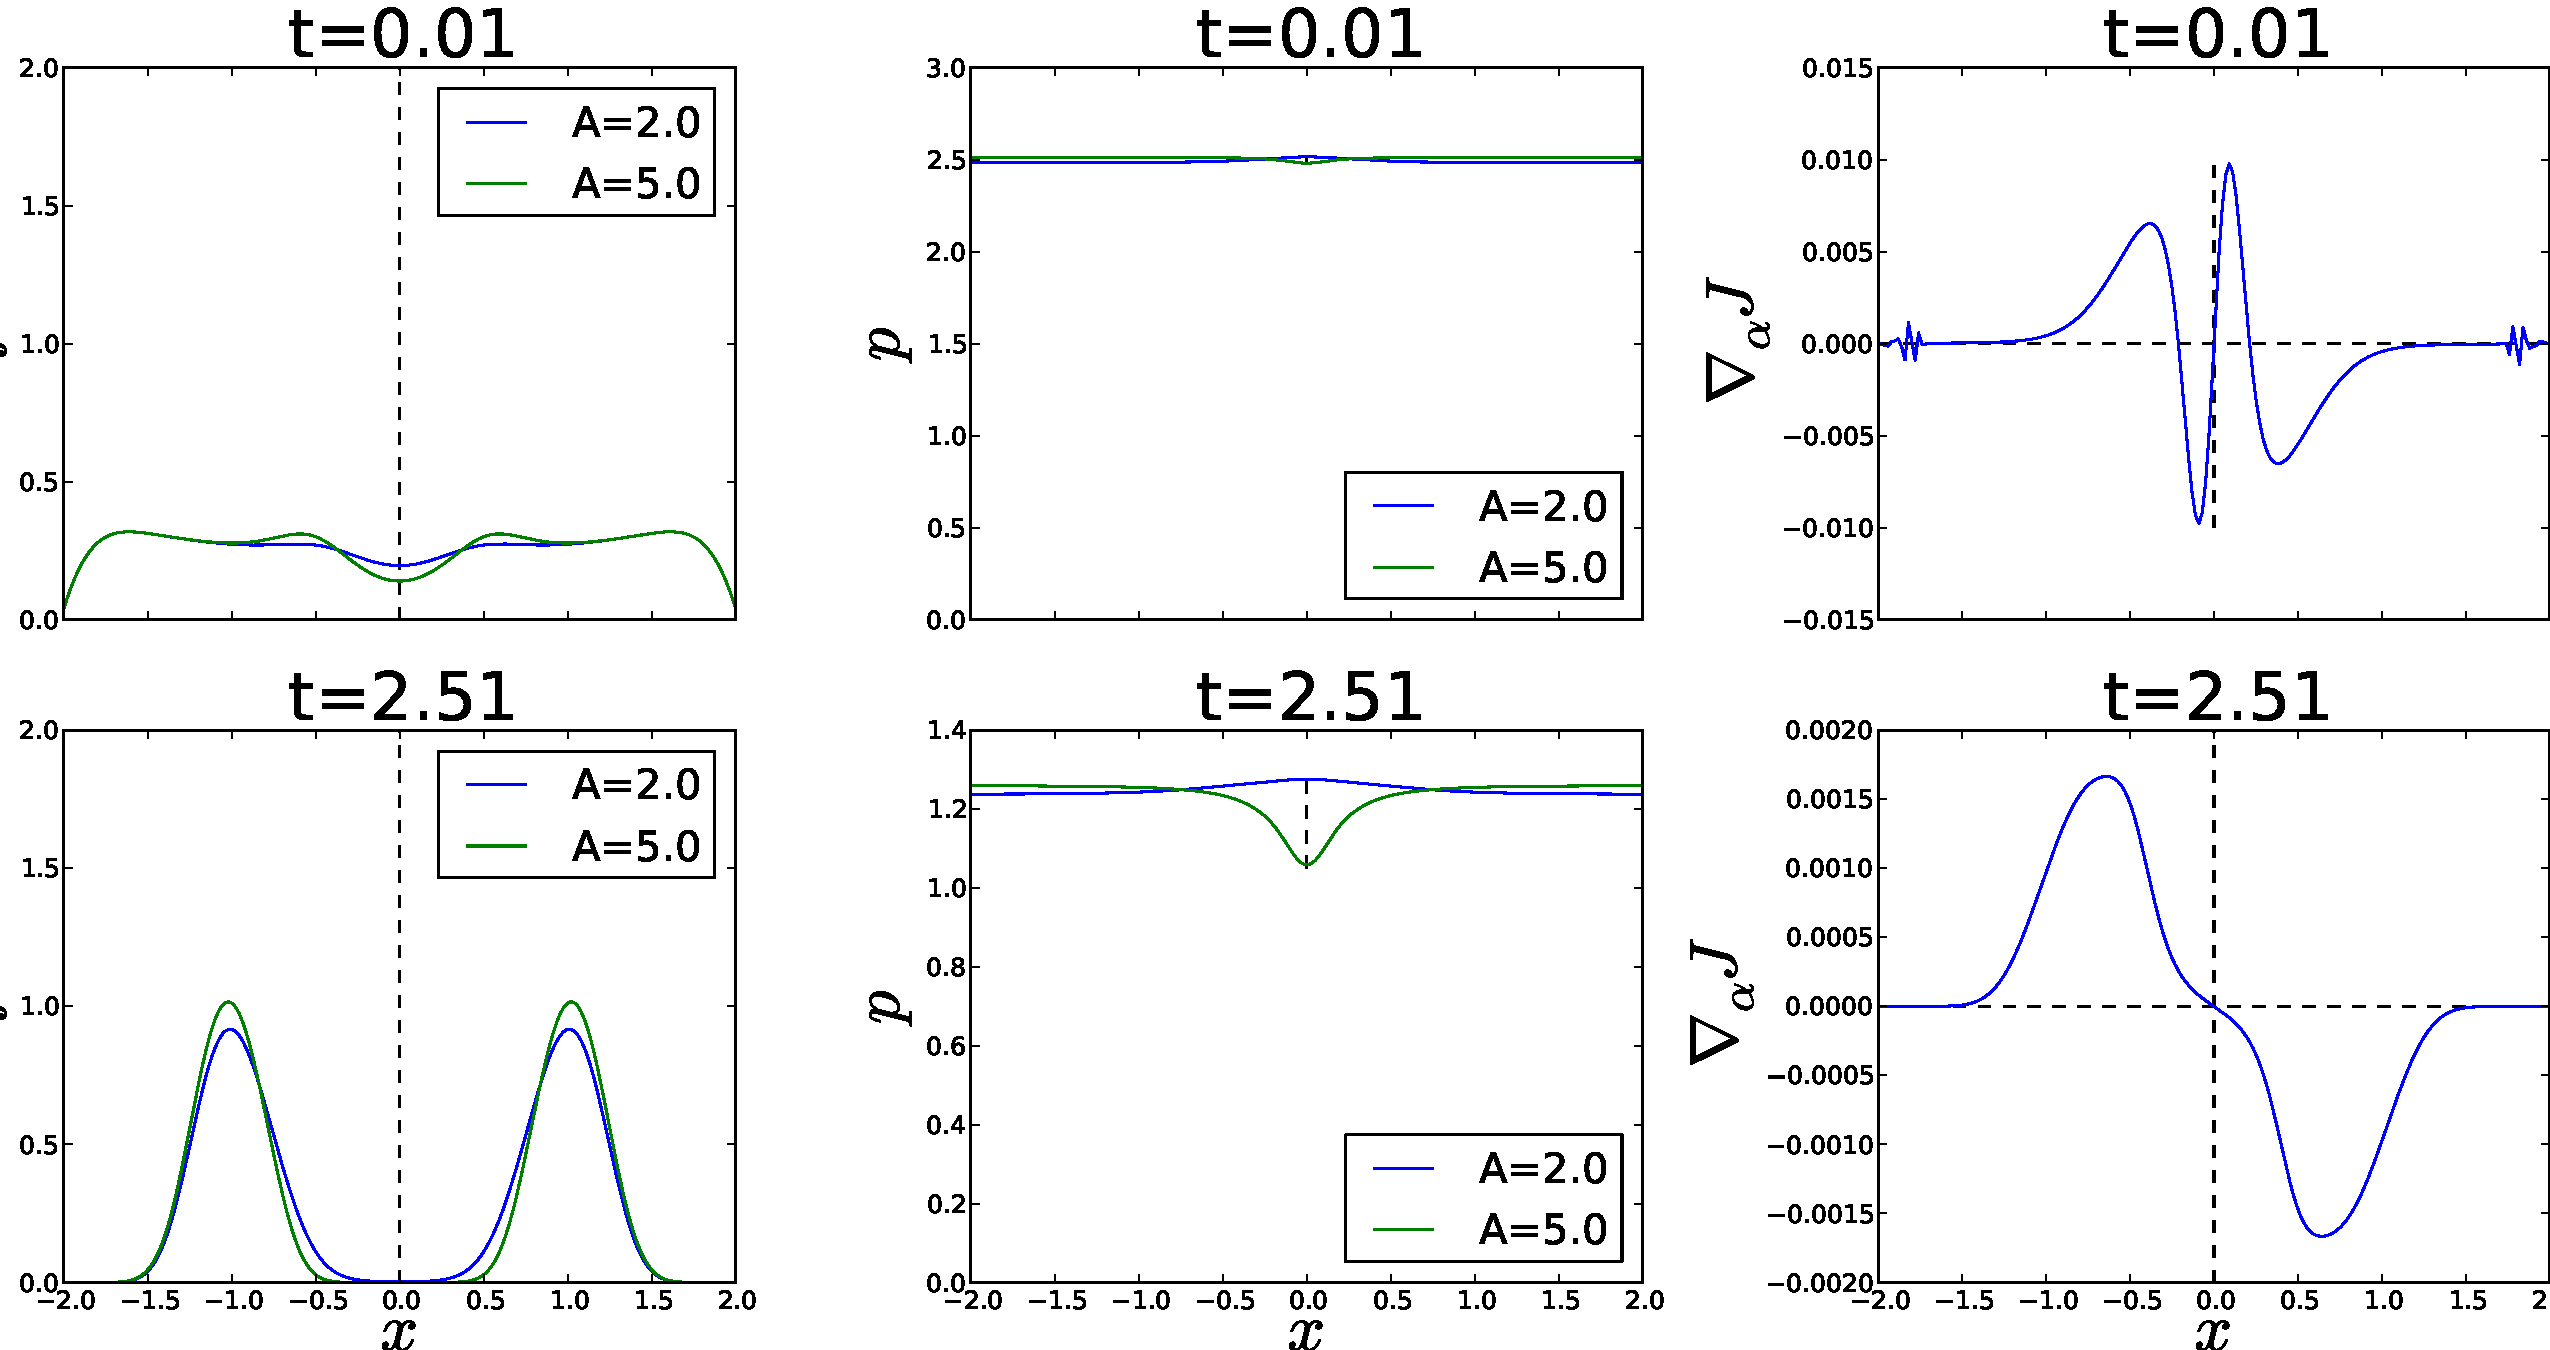
\includegraphics[width=.9\textwidth]{Figs/DoublewellFBSolver/FB_alpha_null_solution_2.pdf}
  \caption[labelInTOC]{Solution to the test Double Well potential problem using
  $\a \equiv 0$. }
  \label{fig:FBSoln_doublewell_alpha_null}
\end{center}
\end{figure} 

\subsubsection{Going through a full gradient descent iteration}
See
\cref{fig:FBSoln_doublewell_alpha_iterations,fig:FBSoln_doublewell_J_iterations},
basically, we are (almost) able to converge to the bang-bang control and from
\cref{fig:FBSoln_doublewell_J_iterations} we are led to believe that the
bang-bang control is indeed optimal. 

\begin{figure}[htp]
\begin{center} 
  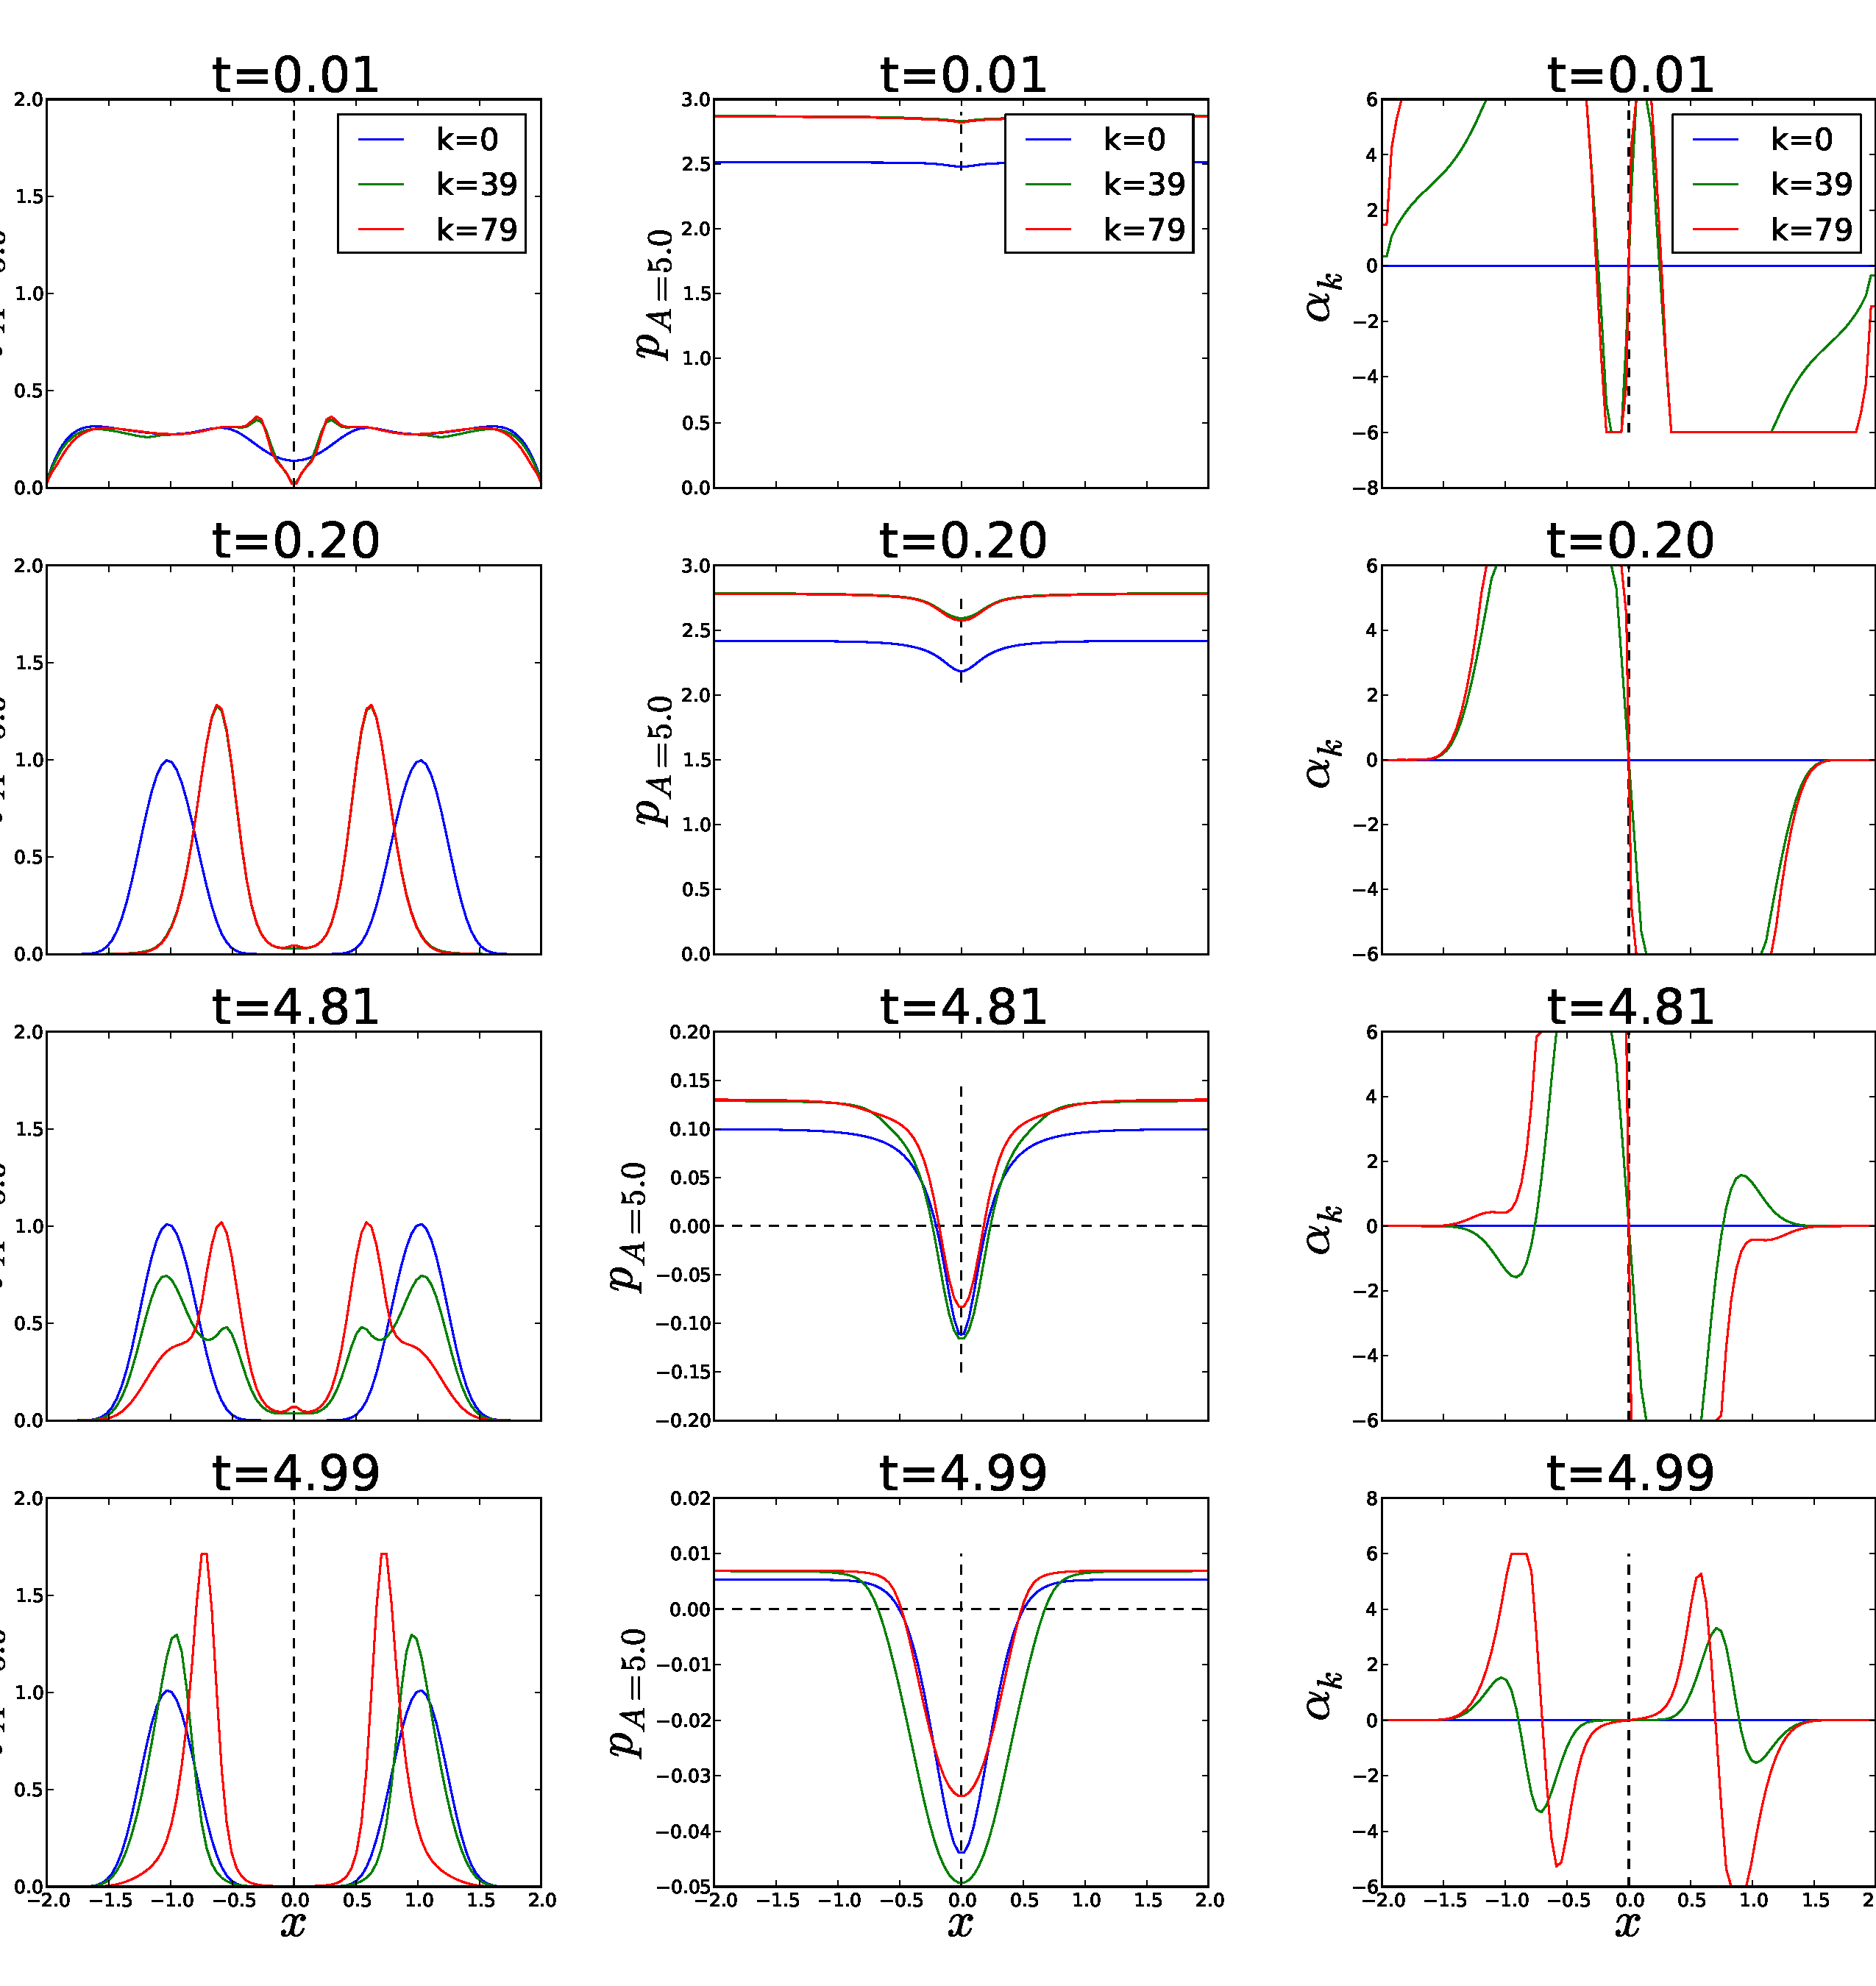
\includegraphics[width=.9\textwidth]{Figs/DoublewellFBSolver/FB_alpha_iterates_uICs_4.pdf}
  \caption[labelInTOC]{Solution to the test Double Well potential problem
  starting from $\a \equiv 0$ until convergence. Note that except at the very
  beginning, $t \approx 0$ and very end of the interval $t\approx T$, we have
  converged to the bang-bang solution. }
  \label{fig:FBSoln_doublewell_alpha_iterations}
\end{center}
\end{figure}

\begin{figure}[htp]
\begin{center}
  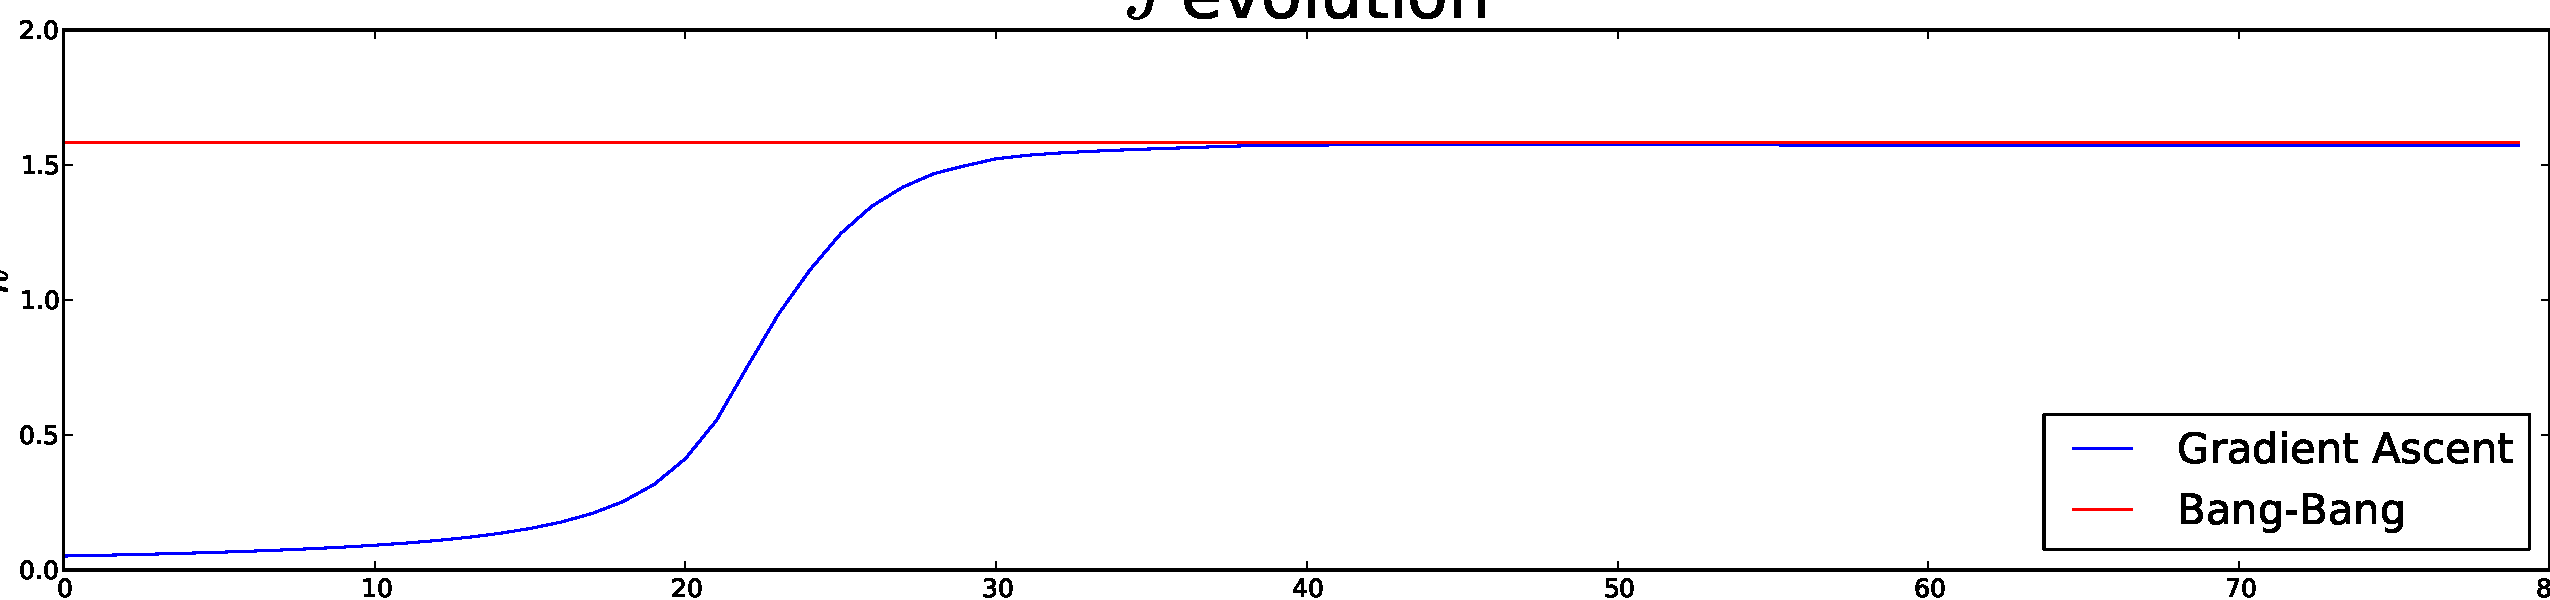
\includegraphics[width=.9\textwidth]{Figs/DoublewellFBSolver/FB_J_iterates_uICs.pdf}
  \caption[labelInTOC]{The evolution of $J$ during the Gradient Ascent, we see
  it goes up and eventually asymptotes with the value of $J$ corresponding to
  the bang-bang control. }
  \label{fig:FBSoln_doublewell_J_iterations}
\end{center}
\end{figure}
 
\clearpage

\section{Second Illustrative Example - the time-constant for the OU model}
\label{sec:MP_OU_TimeDependent}

In \cref{sec:MP_Doublewell_TimeDependent}, we got decent results for the
Double-Well potential problem. Let's now apply the same techniques, (from
\cref{sec:MP_with_a_prior}) on the OU process.

We have seen this a few times, now (\cref{eq:OU_evolution})
$$
dX = \underbrace{(\a + \b( \mu - X)}_{U(x,\a; \th)} \intd{t} +
\underbrace{\s}_{\sqrt{2D}} dW
$$

Since, we've seen the details in \cref{sec:MP_Doublewell_TimeDependent}, we'll
just skip to the chase:

(Known) Parameter values are given by: 

For the fixed parameters we assume $\s = 1. \implies D = 0.5$, $\m = 0$.

For the prior on $\tc = 1/\b$ we use a uniform over $[.5,2]$, which we represent
with only $N_\th = 2$ uniform points located at $[.5,2]$.  

For ICs for the forward density, we take a very broad Gaussian centred at $0$
(the equilibrium).

The control is constrained to lie in the set $[-1 , 1 ]$, i.e.\ $\amax
= 1$. The space is constrained to $x \in [-2.,2.]$, i.e.\ $\xmin, \xmax =
-2.,2.$. 

The $\a_k$ iterates and the gradient-ascent progress of $J$ are shown
in \cref{fig:FBSoln_OU_alpha_iterations,fig:FBSoln_OU_J_iterations}. We see that
again, we converge close to the bang-bang control (which in this case does the
exact opposite than it did in the Double-Well test case). We also see that
the bang-bang control is likely MI-optimal (the red curve in
\cref{fig:FBSoln_OU_J_iterations}). 
 
 
\begin{figure}[htp]
\begin{center} 
  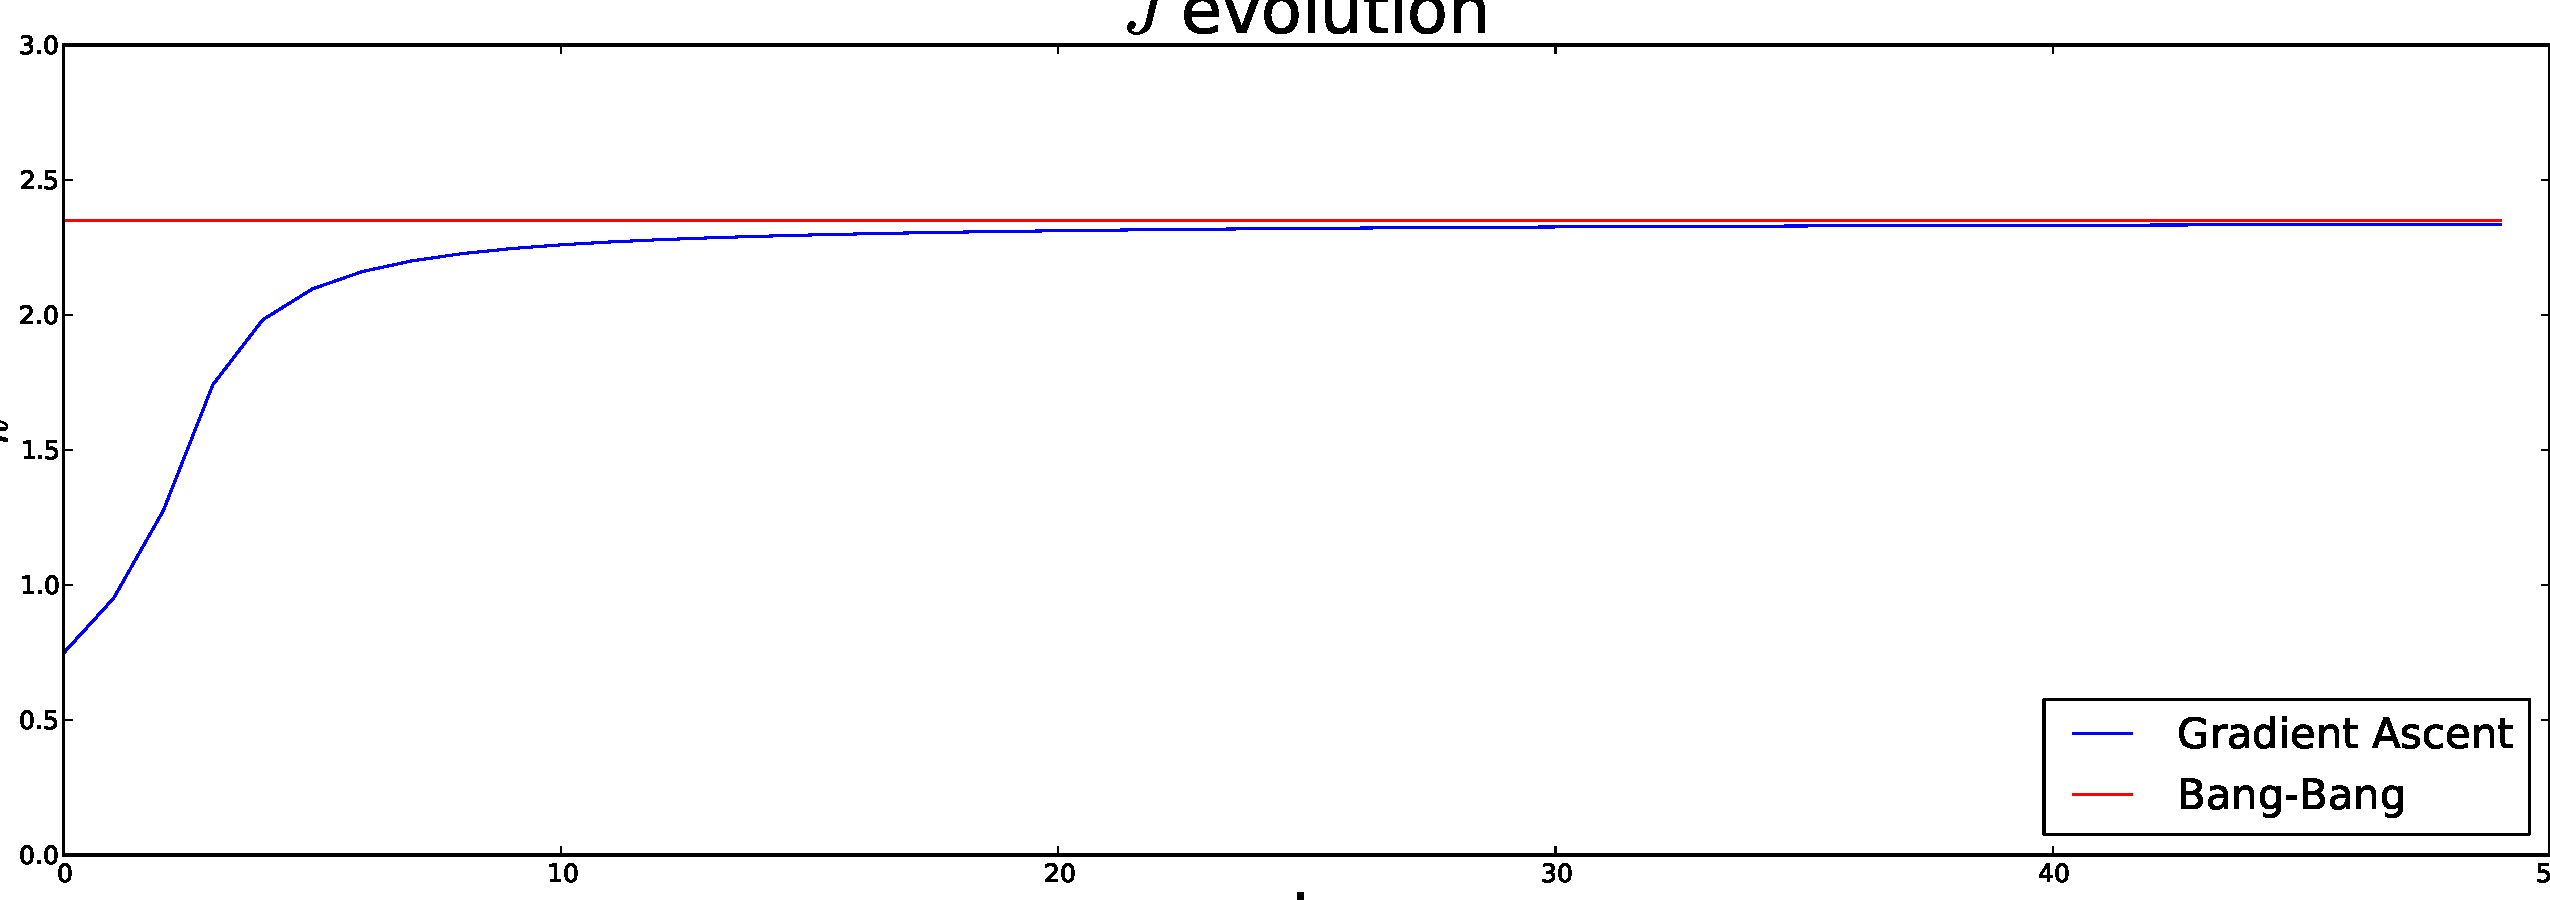
\includegraphics[width=.9\textwidth]{Figs/OUFBSolver/FB_J_iterates_uICs.pdf}
  \caption[labelInTOC]{The evolution of $J$ during the Gradient Ascent
  Ornstein-Uhlenbeck, we see it goes up and eventually asymptotes to the value
  of $J$ corresponding to the bang-bang control.}
  \label{fig:FBSoln_OU_J_iterations}
\end{center}
\end{figure}

\begin{figure}[htp]
\begin{center} 
  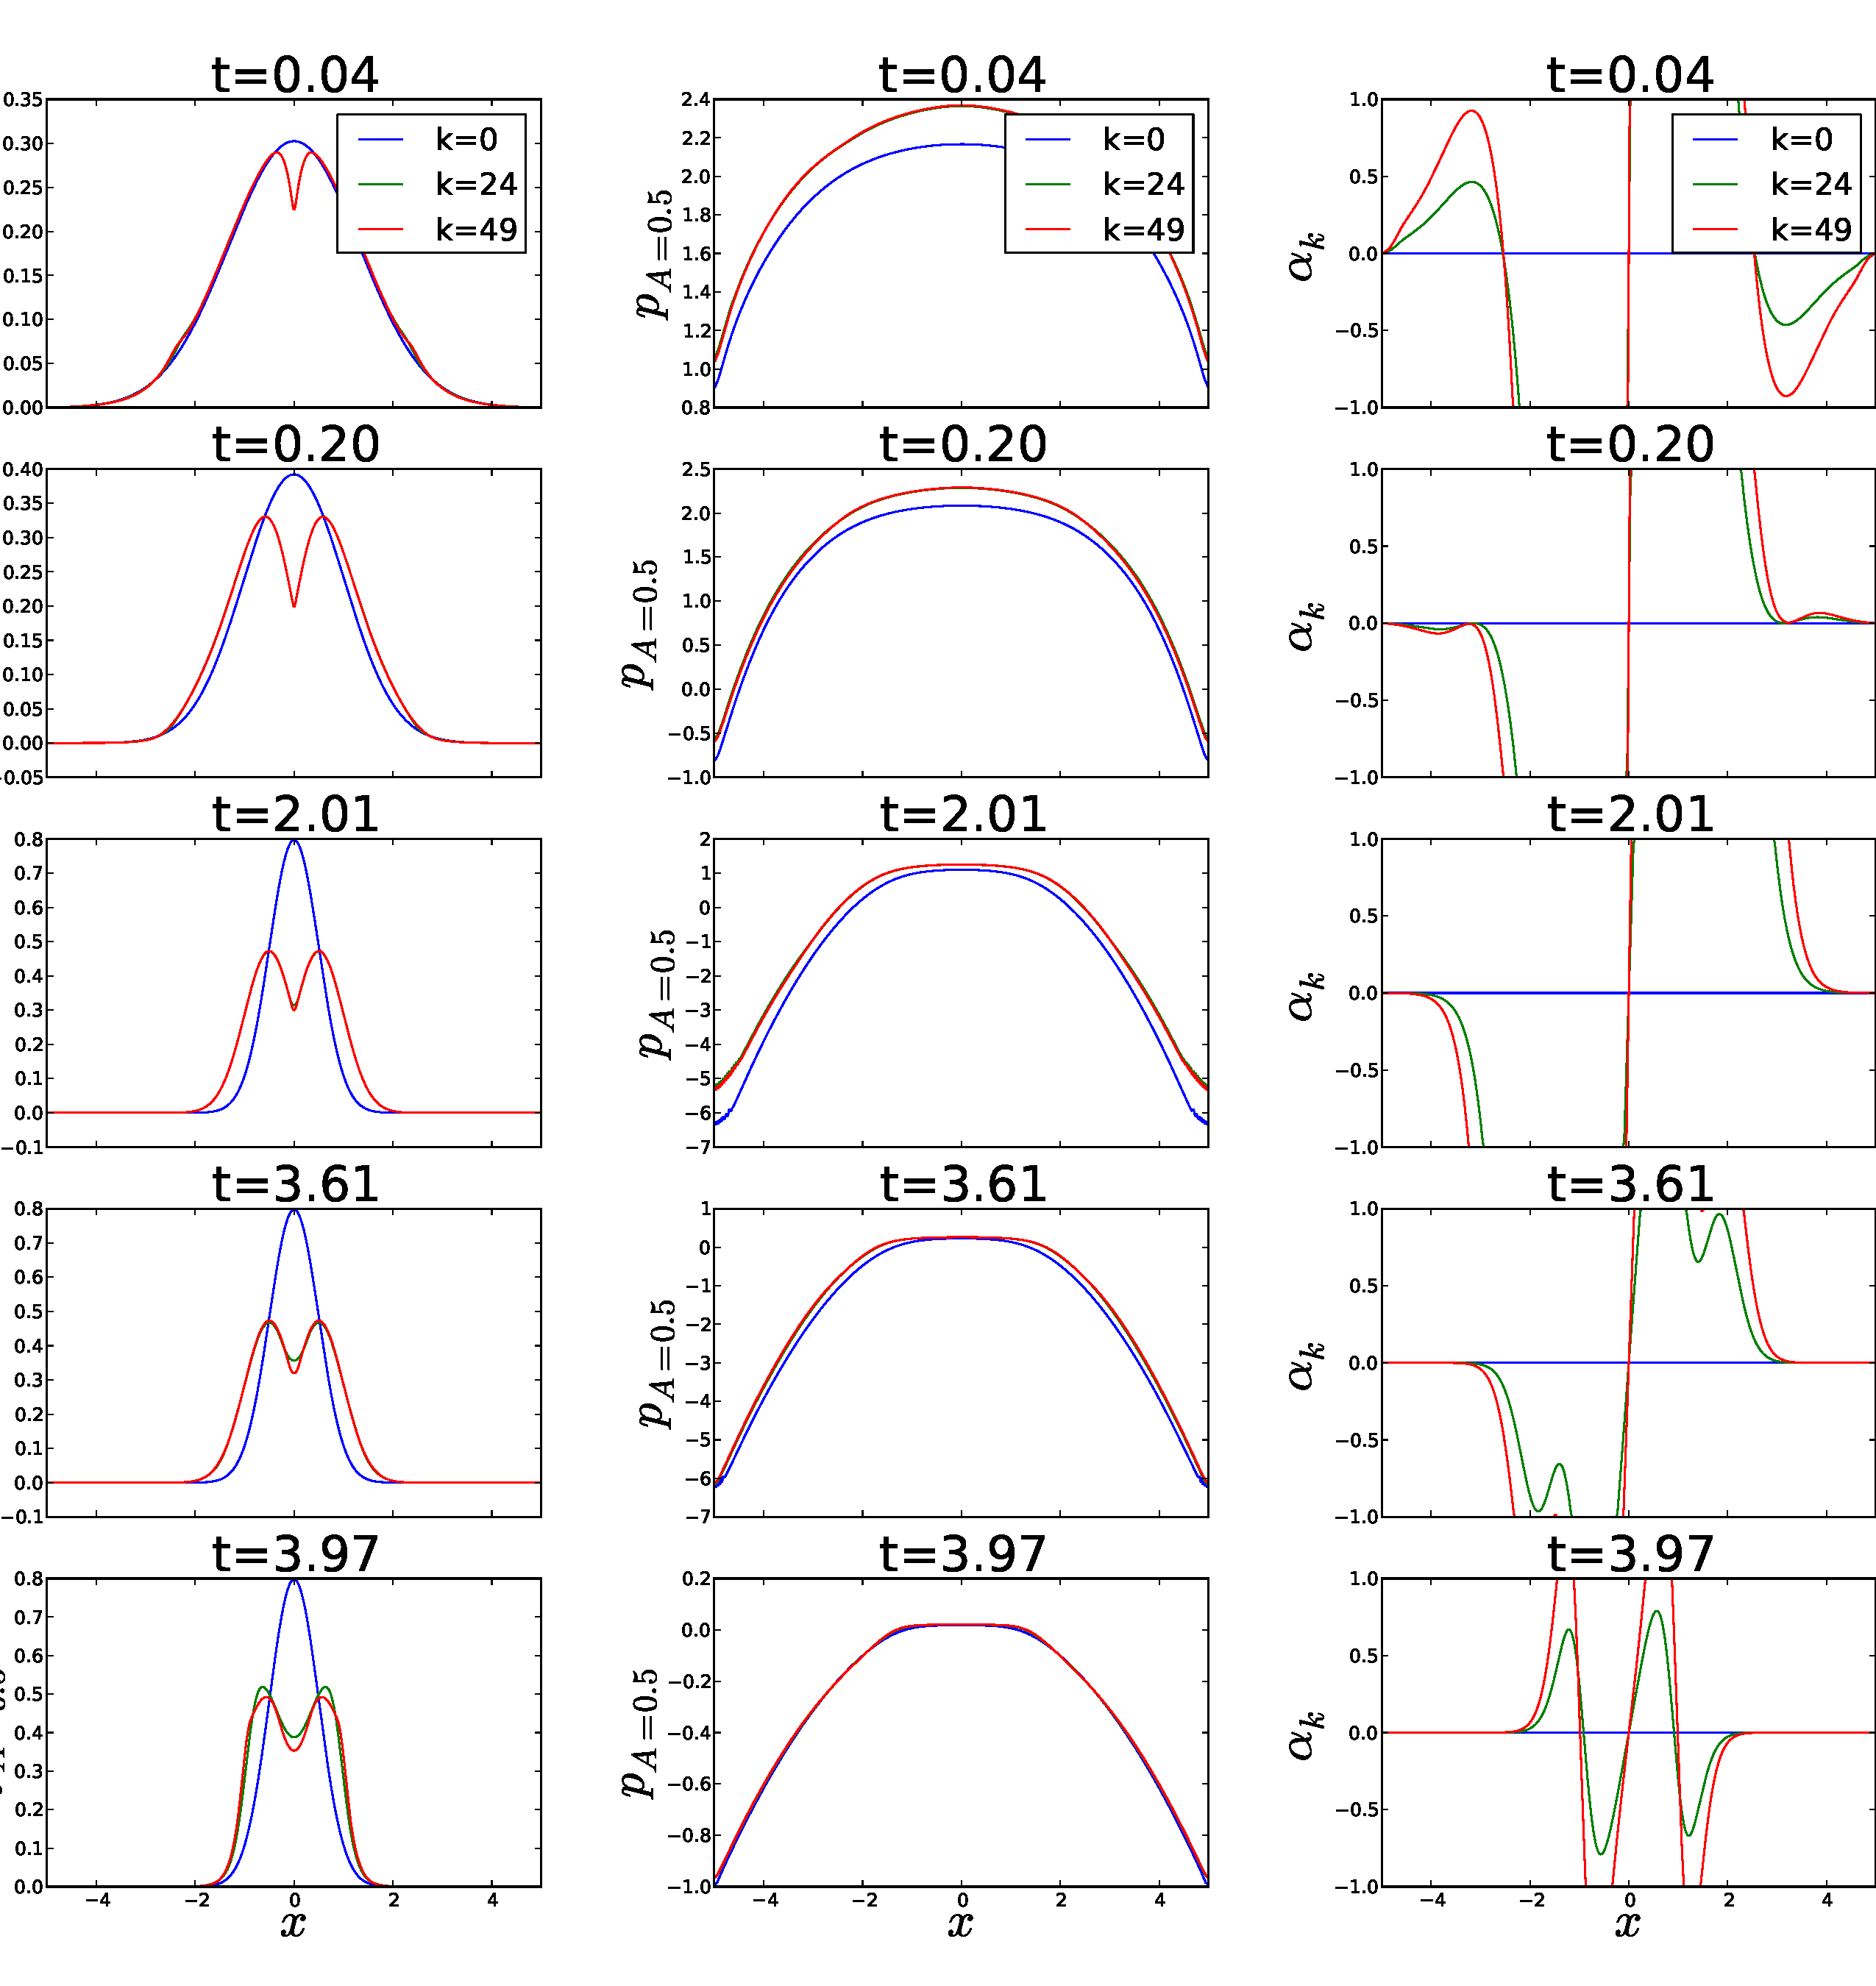
\includegraphics[width=.9\textwidth]{Figs/OUFBSolver/FB_alpha_iterates_uICs_5.pdf}
  \caption[labelInTOC]{Solution to the test Ornstein-Uhlenbeck
  problem starting from $\a \equiv 0$ until convergence. Note that except at the very
  beginning, $t \approx 0$ and very end of the interval $t\approx T$, we have
  converged to the bang-bang solution.}
  \label{fig:FBSoln_OU_alpha_iterations}
\end{center}
\end{figure}


\vskip15pt
\begin{center}

\end{center}

\clearpage

\subsection{Is bang-bang (in space, i.e. feedback) optimal?}
There is some speculation (Susanne!) whether a bang-bang in space control is
optimal. Perhaps a bang-bang control in time is better? In particular a bang-bang control in
space is a feedback control which pulls away from the equilibrium ($\mu=0$,
known) always in the direction depending on the current position of $X_t$. On
the other hand, it might be better to alternatively pull to the left and then to
the right. ('Better' in the sense that one gets better estimates). Let's then
run a simulation comparison. 

On one hand we will take the feedback, MI-optimal bang-bang solution which we
obtained in the beginning of this section (\cref{sec:MP_OU_TimeDependent}). On
the other hand we will divide the time interval in $N$ equal length segments and
alternate Up/Down on each adjacent segment, for illustration see  
\cref{fig:bang_bang_time_vs_space}. When we apply the controls (using identical
streams of random numbers) we get the trajectories shown in
\cref{fig:trajectories_bang_bang_time_vs_space}. We also show the reference
trajectory, using no control at all (labeled 'placebo'). There is obviously
quite a big similarity between all trajectories, since we are using a fairly 
small value of $\amax= 1$.

%\usepackage{graphics} is needed for \includegraphics
\begin{figure}[htp]
\begin{center}
  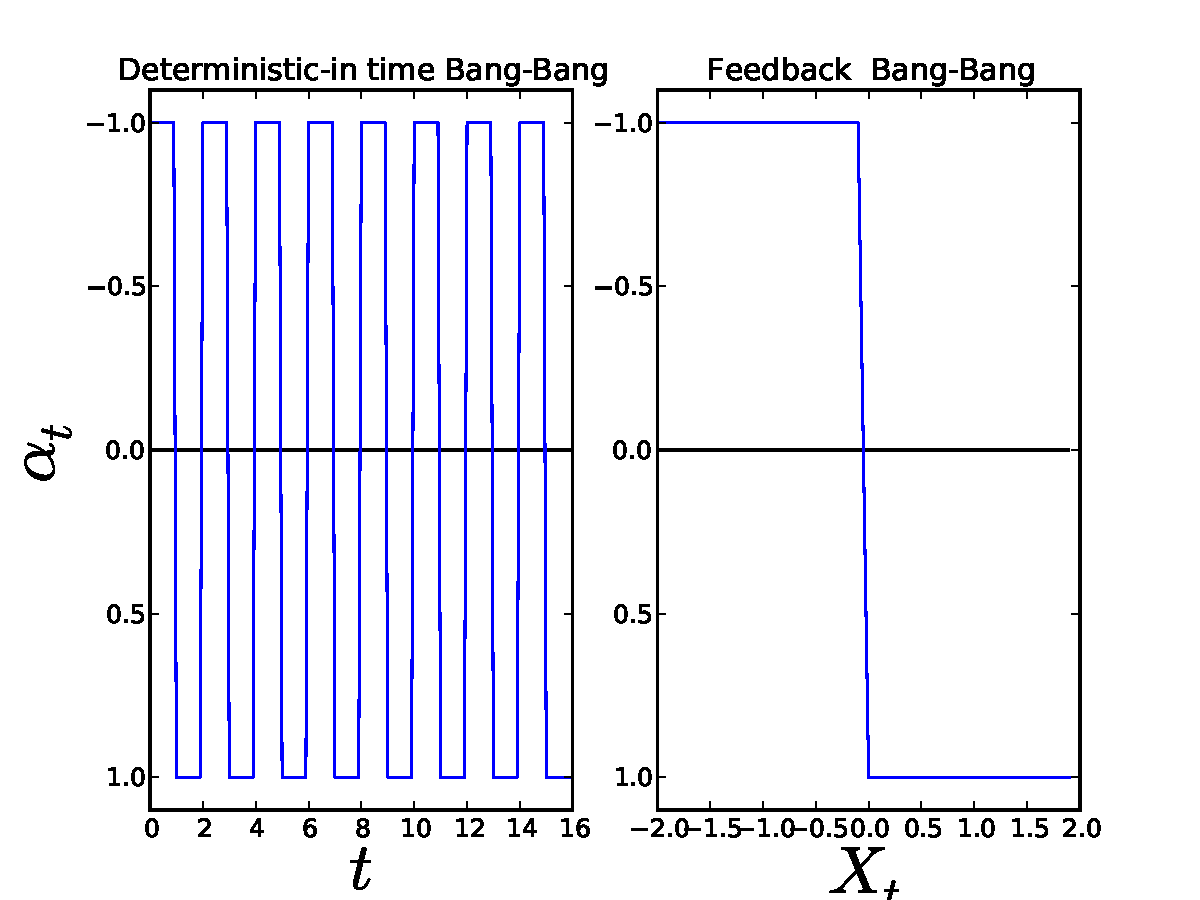
\includegraphics[width=1\textwidth]{Figs/OU_MIControlSimulator/Fb_vs_det_control_illustrate.pdf}
  \caption[labelInTOC]{Illustration of the two competing bang-bang controls,
  space and time}
  \label{fig:bang_bang_time_vs_space}
\end{center}
\end{figure}
%\usepackage{graphics} is needed for \includegraphics
\begin{figure}[htp]
\begin{center}
  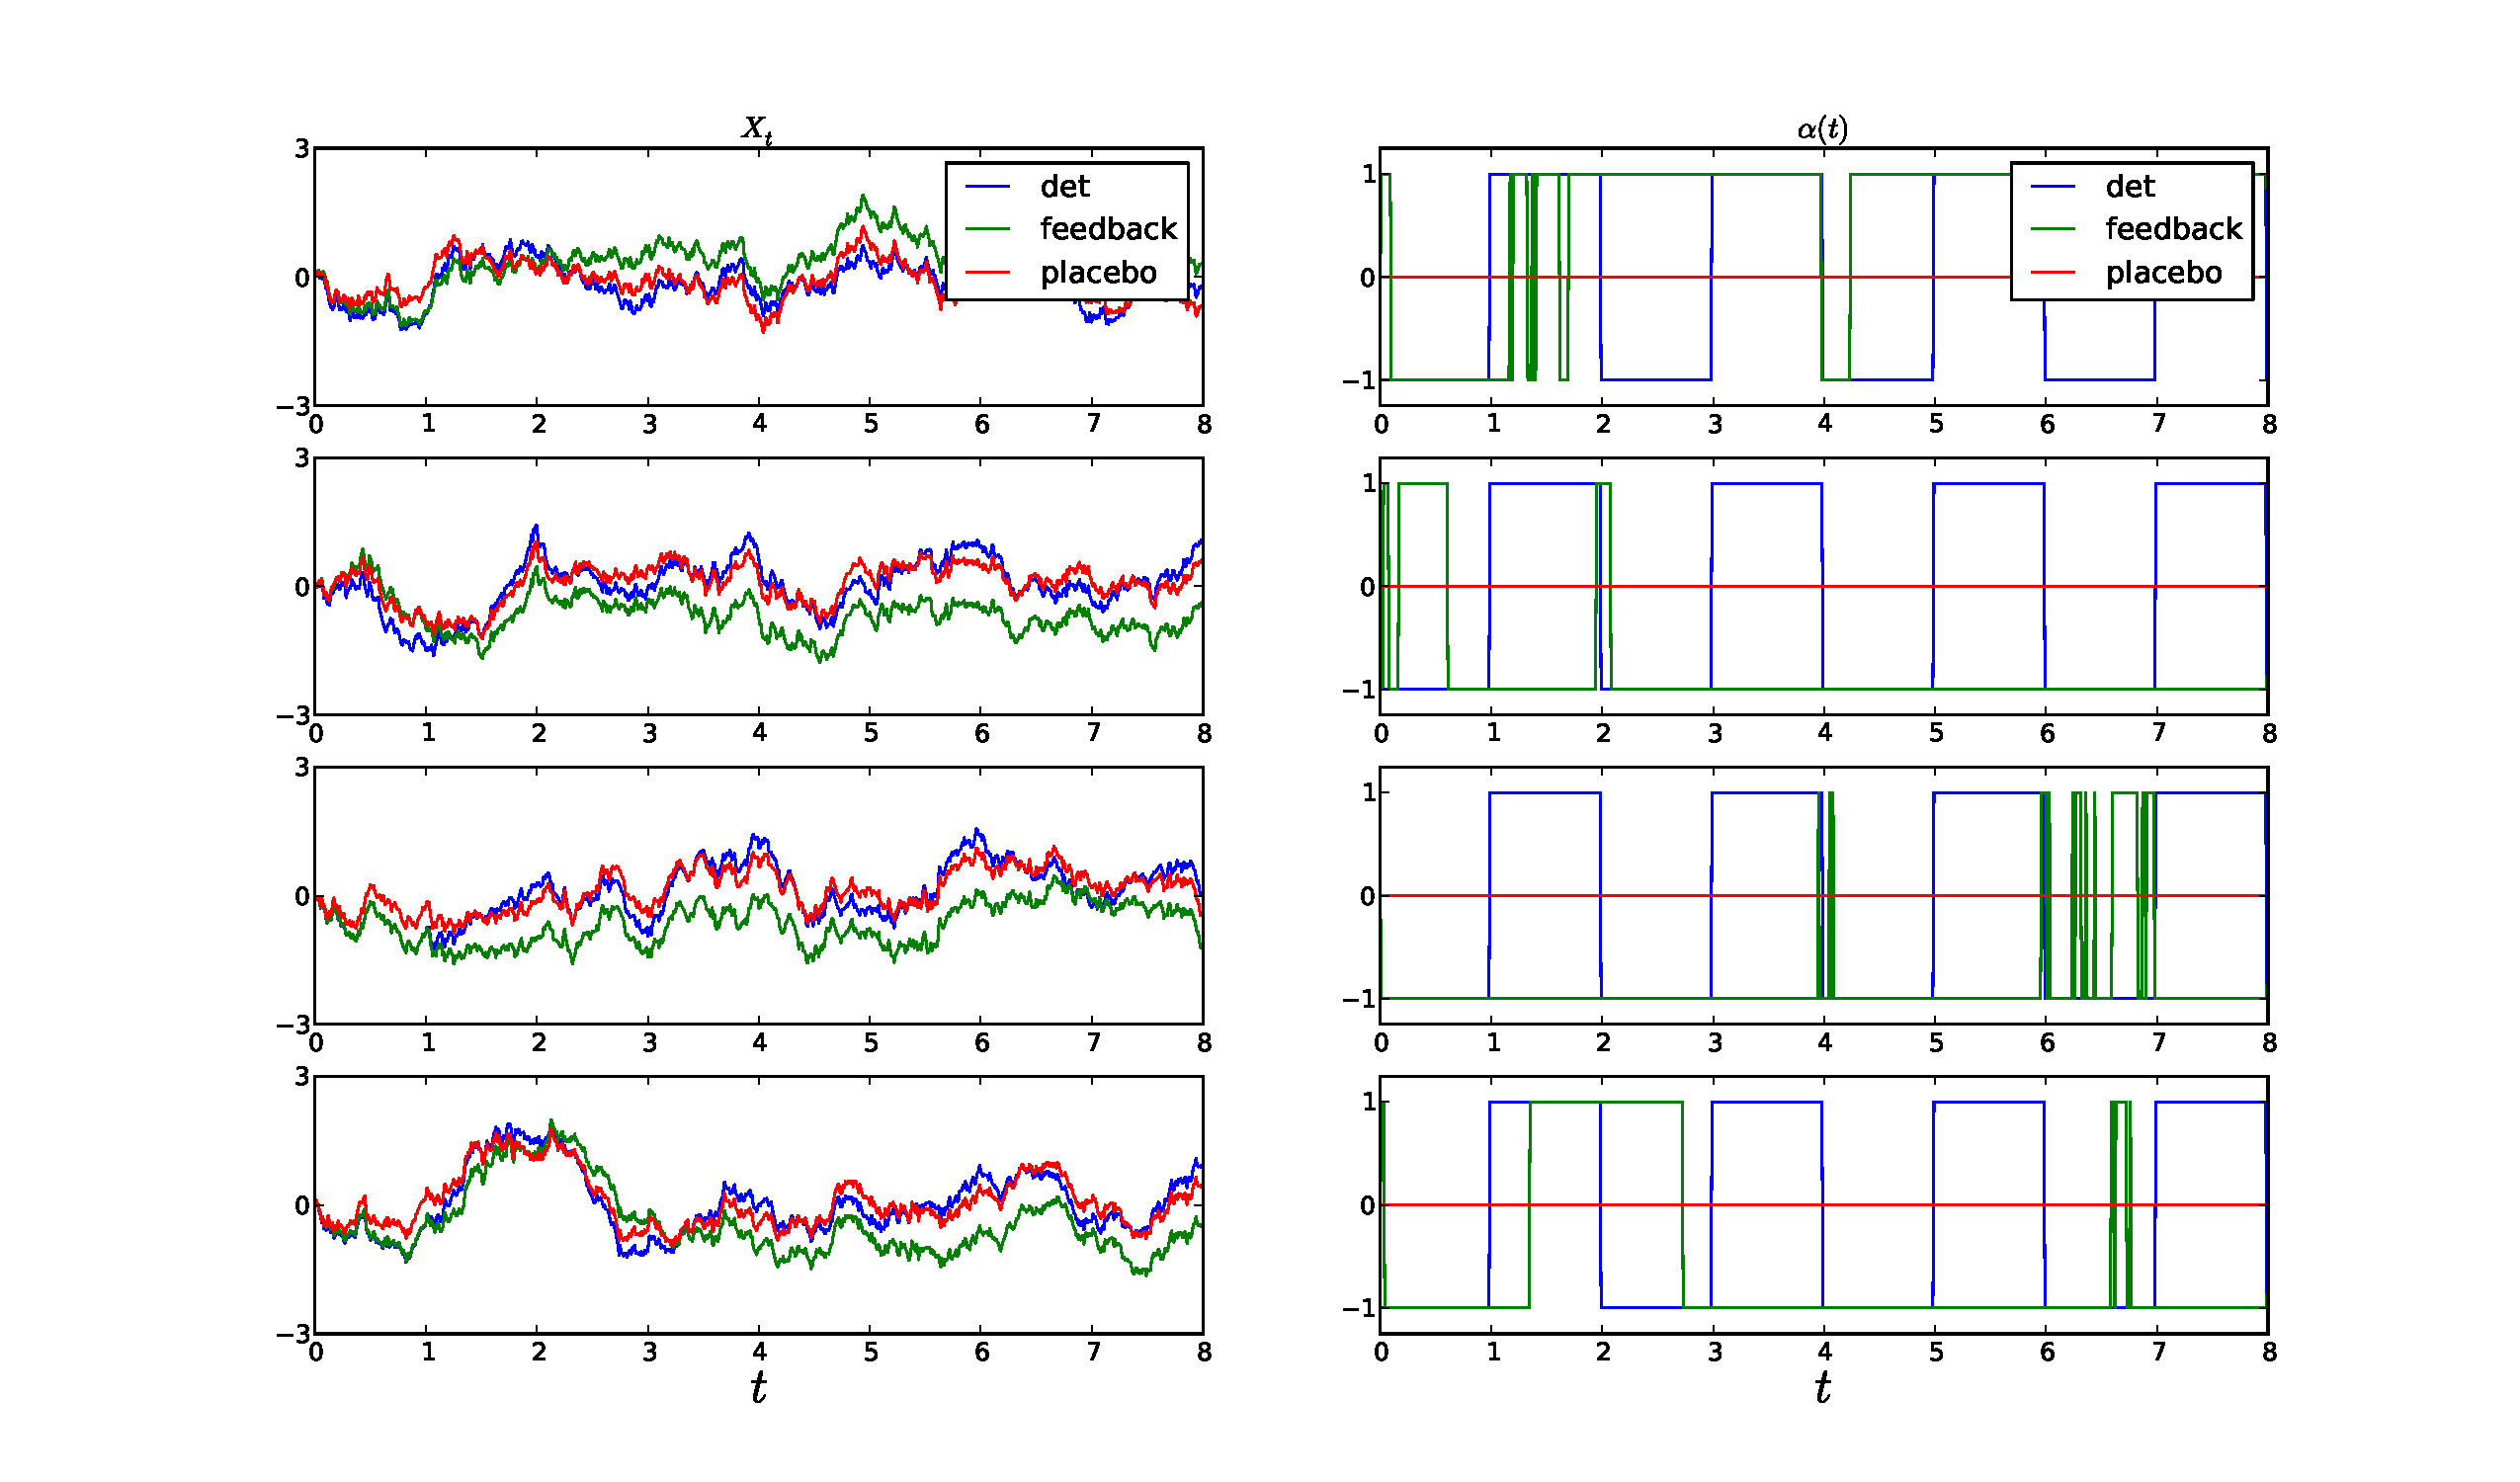
\includegraphics[width=1\textwidth]{Figs/OU_MIControlSimulator/det_vs_fb_amax1.pdf}
  \caption[labelInTOC]{Illustration of the trajectories resulting from the two 
  competing  controls, bang-bang in space and time}
  \label{fig:trajectories_bang_bang_time_vs_space}
\end{center}
\end{figure}



\subsubsection{Estimating $\b$}
We now need a MaxLikelihood formula for $\b$ given the known $\m =0 $ and $\s =
1.$. 
Consider discrete observations ${X_n, t_n}$ obtained at uniform
$t_n$.
Then the transition probabilities $p_n(X_n|X_{n-1})$ are given by:
\begin{align*}
p_n(X_n|X_{n-1}; \b; \a_n, \Delta_n) \propto &
\sqrt{ \frac{\b}{ 1 -  e^{-2\b \Delta_n}}}
\\ &\cdot 
\exp\left(-\frac{\left( X_n - (\frac {\a_n}\b )  - (X_{n-1} -
	 \frac {\a_n}\b) \cdot e^{-\b \Delta_n} \right)^2 \cdot \b}
			{ (1-e^{-2\b\Delta_n})} \right)
\end{align*} 


which makes the log-likelihood look like:

\begin{align*}
l( \b|\ldots) = & \sum \log p_n(X_n|X_{n-1})
\\
=& \frac{N}{2} (\log \b - \log{ (1-e^{-2\b\Delta_n})}
\\ & -\sum_n
{\left(\frac{\left( X_n - (\frac {\a_n}\b )  - (X_{n-1} -
	 \frac {\a_n}\b) \cdot e^{-\b \Delta_n} \right)^2 \cdot \b}
			{ (1-e^{-2\b\Delta_n})} \right)}	 + \const		
\end{align*}

ML estimators for $\b$ are obtained via setting $\di_{\b} l$ to zero.

i.e. we must solve for 
\begin{align}
\di_\b l( \b|\ldots)  
=& \frac{N}{2} \left(\frac 1 \b - 
\frac{2 \Delta_n e^{-2\b\Delta_n}}{(1-e^{-2\b\Delta_n})} \right) \nonumber \\ 
& -\sum_n \textrm{a horrendous mess}  \nonumber
\\
=& 0 
\label{eq:OUML_estimate_beta}
\end{align}


% $$
% \frac{N}{2} \, {\left(\frac{2 \, \Delta e^{\left(-2 \, \Delta
% \beta\right)}}{e^{\left(-2 \, \Delta \beta\right)} - 1} +
% \frac{1}{\beta}\right)}
% $$
where 'a horrendous mess' is actually (using SAGE - python's CAS):
\begin{multline}
-\frac{2 \, {\left(X_{n-1} e^{\left(-\Delta \beta\right)} -
\frac{{\left(e^{\left(-\Delta \beta\right)} - 1\right)}
\a_{n}}{\beta} - X_{n}\right)}^{2} \Delta \beta e^{\left(-2 \,
\Delta \beta\right)}}{{\left(e^{\left(-2 \, \Delta \beta\right)} -
1\right)}^{2}} 
+
\\
 \frac{2 \, {\left(X_{n-1} e^{\left(-\Delta
\beta\right)} - \frac{{\left(e^{\left(-\Delta \beta\right)} - 1\right)}
\a_{n}}{\beta} - X_{n}\right)} {\left(\Delta X_{n-1}
e^{\left(-\Delta \beta\right)} - \frac{\Delta \a_{n} e^{\left(-\Delta
\beta\right)}}{\beta} - \frac{{\left(e^{\left(-\Delta \beta\right)} -
1\right)} \a_{n}}{\beta^{2}}\right)} \beta}{e^{\left(-2 \, \Delta
\beta\right)} - 1} -
\\ \frac{{\left(X_{n-1} e^{\left(-\Delta
\beta\right)} - \frac{{\left(e^{\left(-\Delta \beta\right)} - 1\right)}
\a_{n}}{\beta} - X_{n}\right)}^{2}}{e^{\left(-2 \, \Delta
\beta\right)} - 1}
\end{multline}

!!!
Once that is all done, we can compute some estimates for the trajectories
from \cref{fig:trajectories_bang_bang_time_vs_space} and tabulate those in
\cref{tab:OU_control_estimates_bang_bang_time_vs_space}. Although not
substantially, the feedback bang-bang control is clearly superior as it has a 
lower bias and a lower variance than the estimates obtained when using the
deterministic, bang-bang in time, control. I've tried with other values for the
switching frequency of the deterministic control (switch every .5, 1, 2
time units) and the results do NOT change. I've also tried with tweaking the
value of $\alpha_{max}$, again, same results. 

In \cref{tab:OU_control_estimates_bang_bang_time_vs_space}, we also show the
results for the base-case (called 'placebo') where $\a(x,t) \equiv 0$.

\begin{table}
\begin{tabular}{l|ccc}
$T_f$:
 & 8
 & 16
 & 32
\\
placebo :
 & (1.41, 0.66)
 & (1.19, 0.41)
 & (1.09, 0.27)
\\
det :
 & (1.37, 0.60)
 & (1.16, 0.37)
 & (1.08, 0.24)
\\
feedback :
 & (1.29, 0.39)
 & (1.14, 0.24)
 & (1.06, 0.15)
\\
\end{tabular}
\caption{(Mean/st.deviation) of the $\b$- ML Estimates obtained using the three
controls, given different value for $T_f$. Although not substantially, the
bang-bang feedback control is clearly superior as it has a lower bias and a
lower variance. We have used $N_{traj} = 1000$ to form the statistics for each
$T_f$ and control. The 'true' value is $\b = 1.$}
\label{tab:OU_control_estimates_bang_bang_time_vs_space}
\end{table}


Finally, in \cref{fig:ML_beta_root}, we show something that might be of
interest. It is the graph of the score function of the $\b$ ML estimates,
$\di_\b l$, \cref{eq:OUML_estimate_beta} as a function of $\b$ for several
different trajectories ${X_n}$. Recall that an estimate is obtained by finding
the solution to $\di_\b l(\b) = 0$. What we see is that the
root function corresponding to the feedback control, tends to be much steeper. Intuitively, I associate this
with a more robust estimation process, since small vertical perturbations will
have small effects on the root $\b$, while for the flatter curves (the ones
corresponding to the placebo and the deterministic control), small vertical
perturbations will much more drastically change the $\b$ estimate.
 
%\usepackage{graphics} is needed for \includegraphics
\begin{figure}[htp]
\begin{center}
  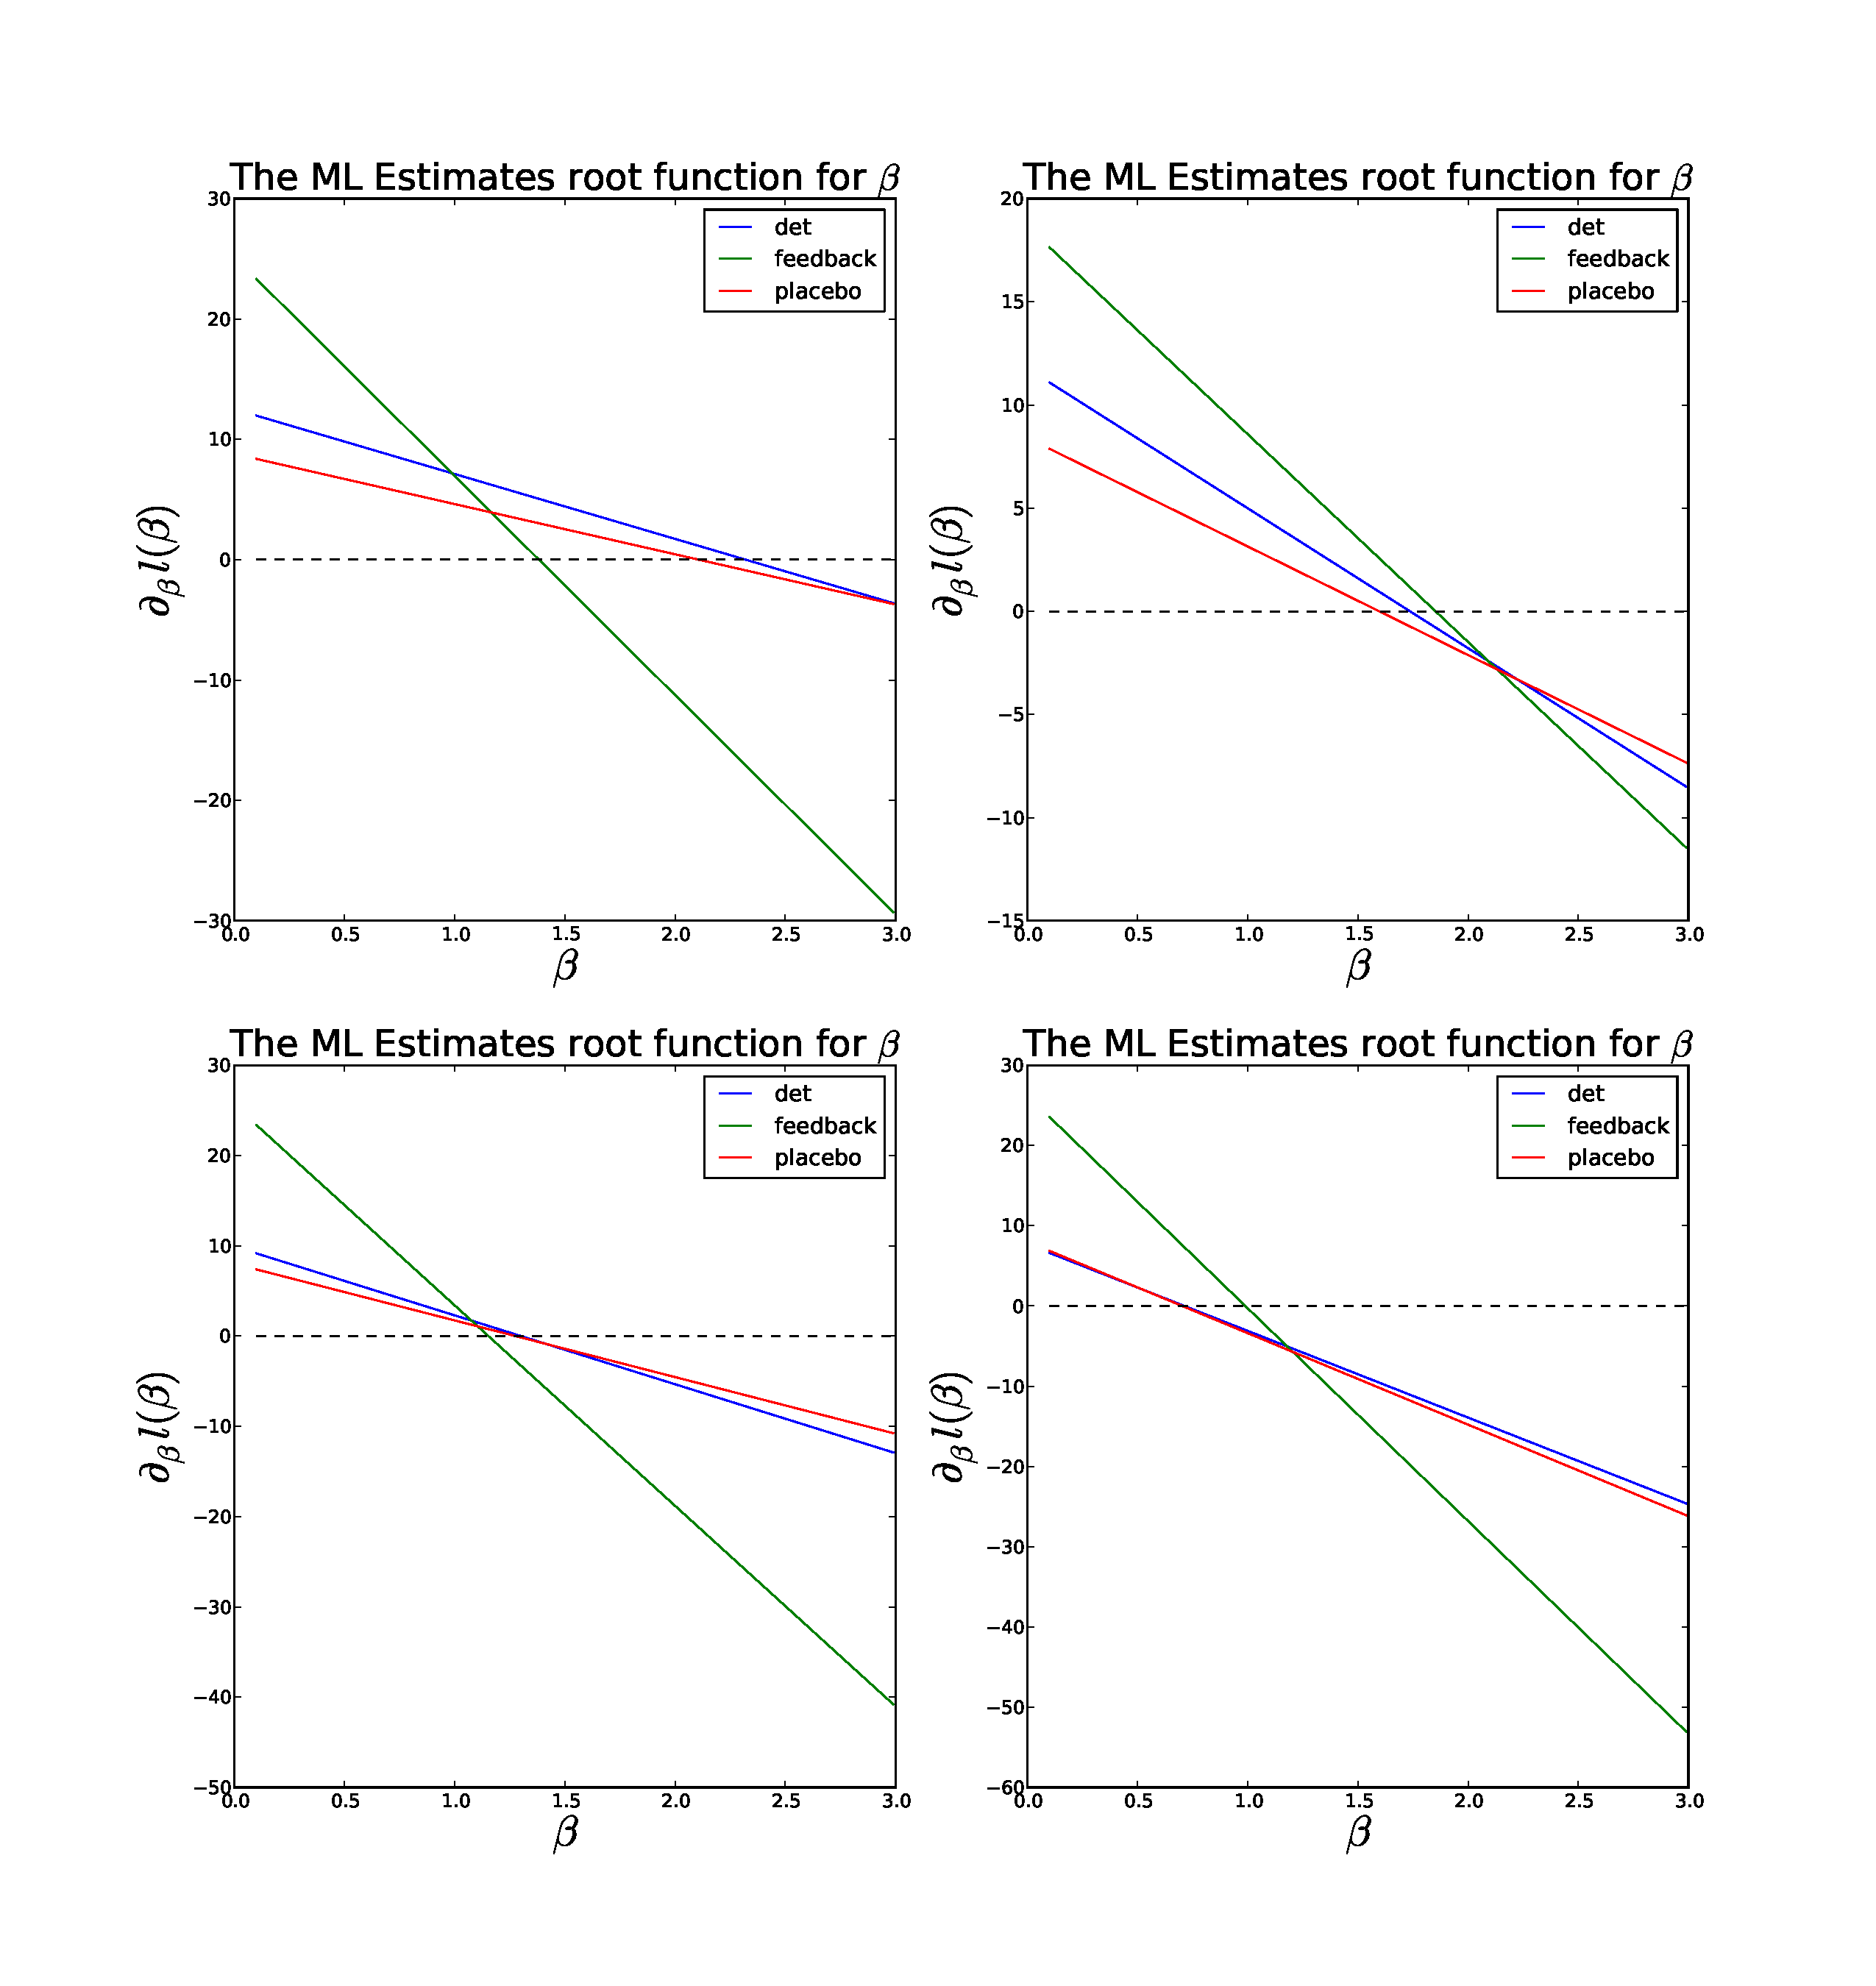
\includegraphics[width=1\textwidth]{Figs/OU_MIControlSimulator/BetaRoot_Tf=16.pdf}
  \caption[labelInTOC]{THe root function \cref{eq:OUML_estimate_beta} for a few
  trajectories}
  \label{fig:ML_beta_root}
\end{center}
\end{figure}



\subsubsection{Sweep through $\b_{true}, \sigma $}

For completeness we repeat the exercise above, i.e. we recalculate the results
from \cref{tab:OU_control_estimates_bang_bang_time_vs_space} for several
different values of the 'true' value of $\b$ and of $\sigma$. See
\cref{tab:betasigma_sweep_for_ML_estimation_of_OU}

\begin{table}
\begin{tabular}{l|cccccc}
\input{../OptEstimate/Figs/OU_MIControlSimulator/betasigmasweep_tabulate.txt}
% $(\beta_{true}, \sigma)$: & (5.00,0.25) & (5.00,4.00) & (1.00,0.25) &
% (1.00,4.00) & (0.20,0.25) & (0.20,4.00)\\ \hline placebo: & (68.67, 9.09, 0) &
% (0.34, 0.08, 0) & (17.90, 6.15, 0) & (0.10, 0.05, 0) & (6.00, 3.77, 0) & (0.06, 0.05, 2)\\det: & (19.62, 2.04, 0) & (0.41, 0.11, 0) & (5.40, 0.81, 0) & (0.11, 0.07, 3) & (2.51, 0.88, 0) & (0.06, 0.05, 4)\\feedback: & (14.83, 1.32, 0) & (0.89, 0.10, 0) & (1.59, 0.13, 0) & (0.34, 0.08, 0) & (0.34, 0.02, 0) & (0.18, 0.06, 0)\\
\end{tabular}
\caption{Sweep through the $\b_{true}, \sigma $ parameters and the effect on
the estimates. $Tf =16$. We've used $N=100$ to form the statistics. In
brackets are displayed the mean estimate (out $N$) and the estimates standard
deviation. We have set the initial value to $X_0=2.$, if we set it to $X_0 =
.0$ the feedback-based estimator will be much more dominant, especially for low
noise, presumably because for low noise  the other systems spend too much
time near the equilibrium if they already start there, and being near
equilibrium there is no restoring force and thus $\b$ is harder to estimate...}
\label{tab:betasigma_sweep_for_ML_estimation_of_OU}
\end{table}


\clearpage



\subsection{Multi-Parameter Case}
So far, we have worked in the simplest possible context - with only one unknown
parameter. Let's try to ramp it up a bit to TWO unknown parameters. In the OU
case this means, $\{\b, \m\}$. 

WAIT! First let's consider if we only had $\m$ uncertainty? Suppose we
knew $\b = 1$ and only cared about $\mu$, which could be one of ${-1,1}$. Then, after some
crunching it turns out (Results NOT shown) that the best thing to do is do
nothing, $\a \equiv 0$. I don't know why, but that is what the numerics
suggest\ldots. Again, by 'best thing' we mean the control, $\a(x,t)$,
which maximizes $J[\a]$ in \cref{eq:mutual_info_time_integrated}. 

So as a first guess, the optimal control for when both $\b,\m$ are uncertain
should be some combination of 'bang-bang' and 'null'. Bang-bang is best for $\b$
and 'null' (do nothing/ $\a=0$) is (we think) best for $\m$.
We let the prior be equally weighted between the following (cartesian
-product ) possibilities:
$$
(\b, \m) =\{.5, 2\} \times \{-1,1\} = (.5,-1), \ldots (2,1)
$$
i.e.\ in the prior, each of the 4 possibilities has probability
0.25. The calculations after that are exactly as in the earlier section when we only had
an uncertainty over $\b$. We show the distributions and optimal control in
\cref{fig:fpalpha_iterates_mubeta} and the objective value in
\cref{fig:OU_mubeta_Jiterates}. 

Strictly speaking, what we see is quite novel and interesting! The optimal
control is a strange combination of 'bang-bang' outside for  $x \notin [-1,1]$.
But null ($\a=0$.), for $x in [-1,1]$. This is slightly cheating, as we take
that that to be the case as initial guess (for $\a_k$) and if we started from
different initial guess for $\a_k$ we will not be able to converge to this,
although, that is likely more a fault of the gradient algorithm\ldots

However, we see that the difference is really very small. WHereas in the $\b$
uncertainty only,   \cref{fig:FBSoln_OU_J_iterations}, we could triple the value
of the objective, $J$ by going from the initial guess ($\a=0$) to the optimal
control, here the difference between bang-bang, do-nothing, and optimal control
is very, very slight!

Uf!


%\usepackage{graphics} is needed for \includegraphics
\begin{figure}[htp]
\begin{center}
  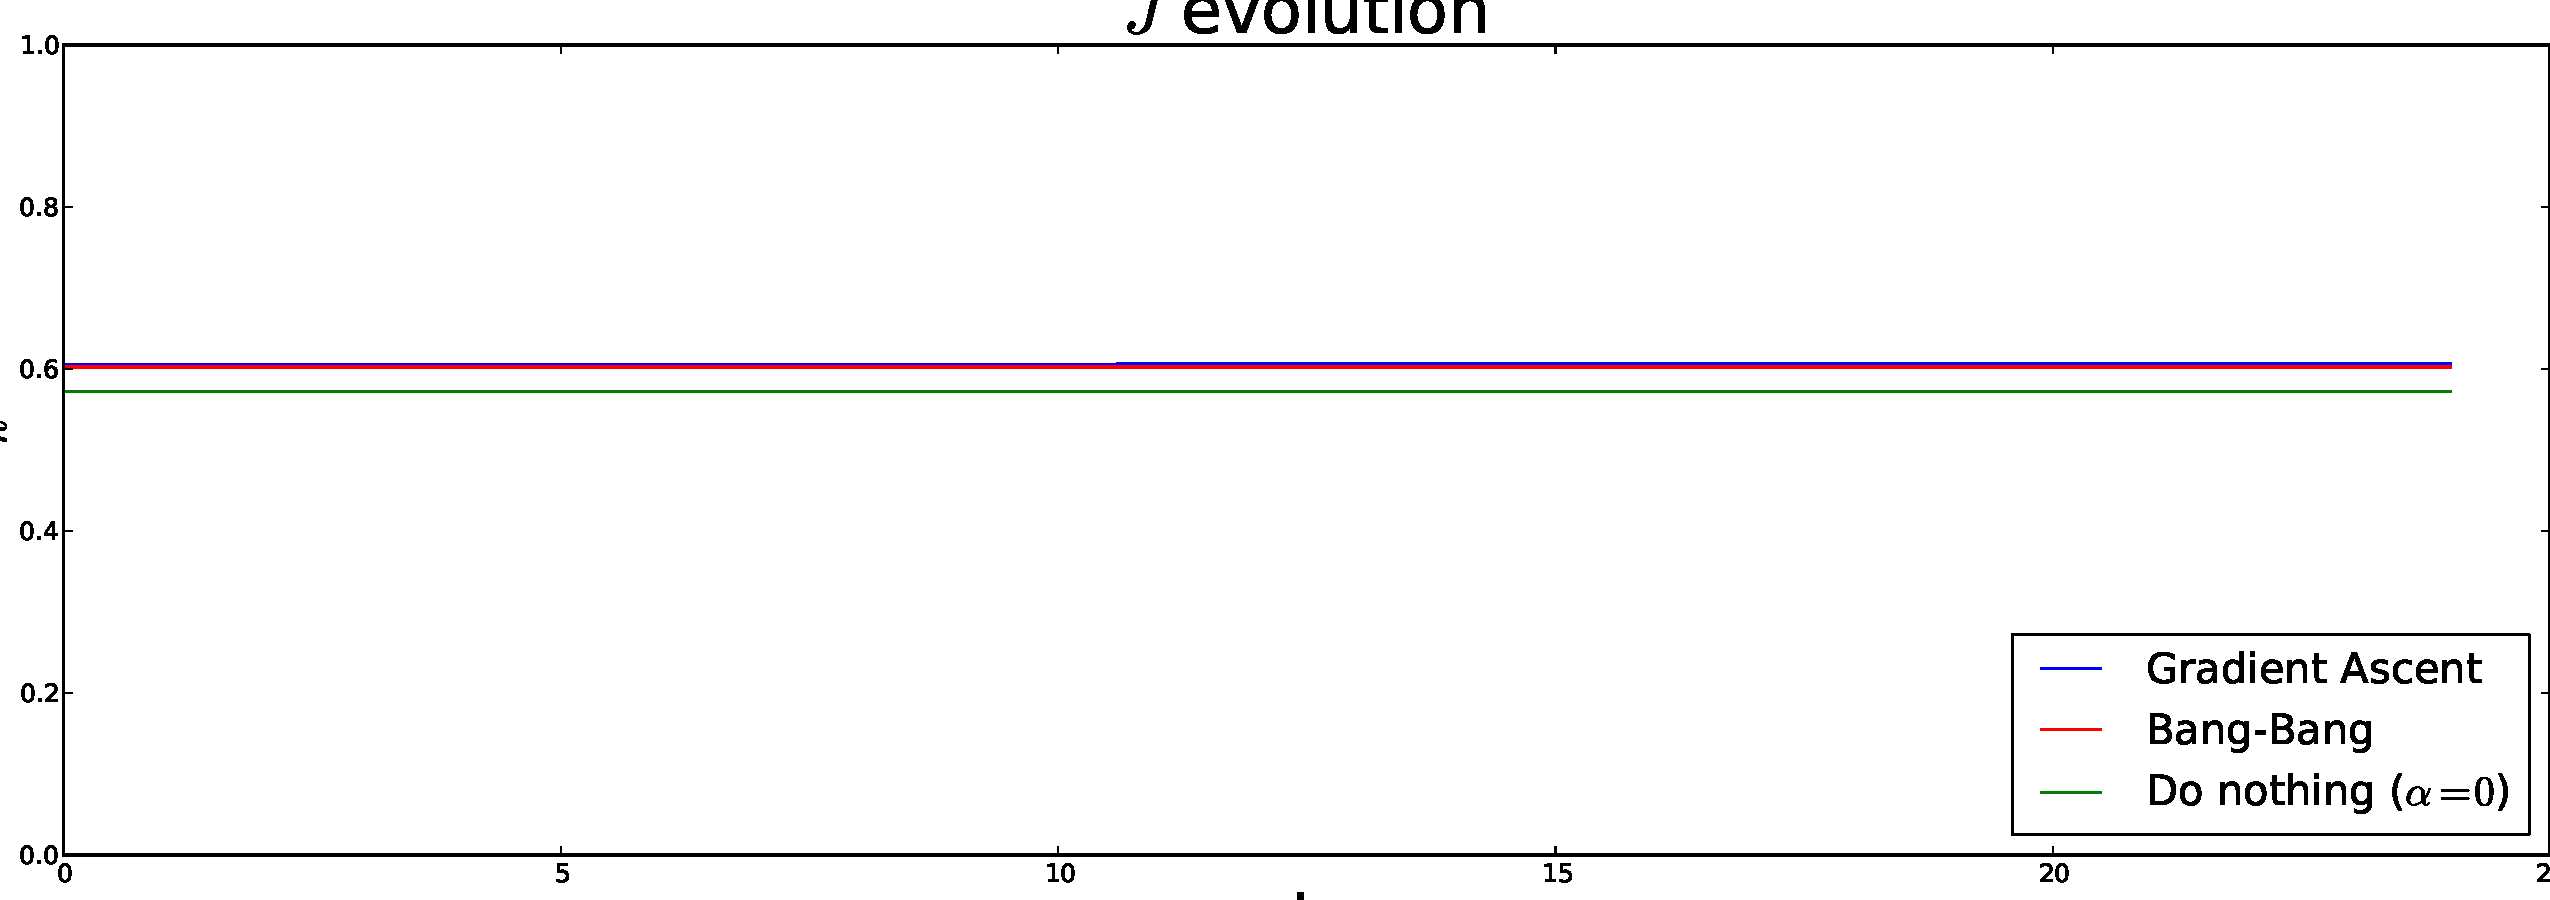
\includegraphics[width=1\textwidth]{Figs/OUFBSolver_BetaMu/FB_J_iterates_uICs_Tf=2.pdf}
  \caption[tableofCs]{The iterations for $J$ when both $\tc, \m$ are
  uncertain.}
  \label{fig:OU_mubeta_Jiterates}
\end{center}
\end{figure}

\begin{figure}[htp]
\begin{center}
  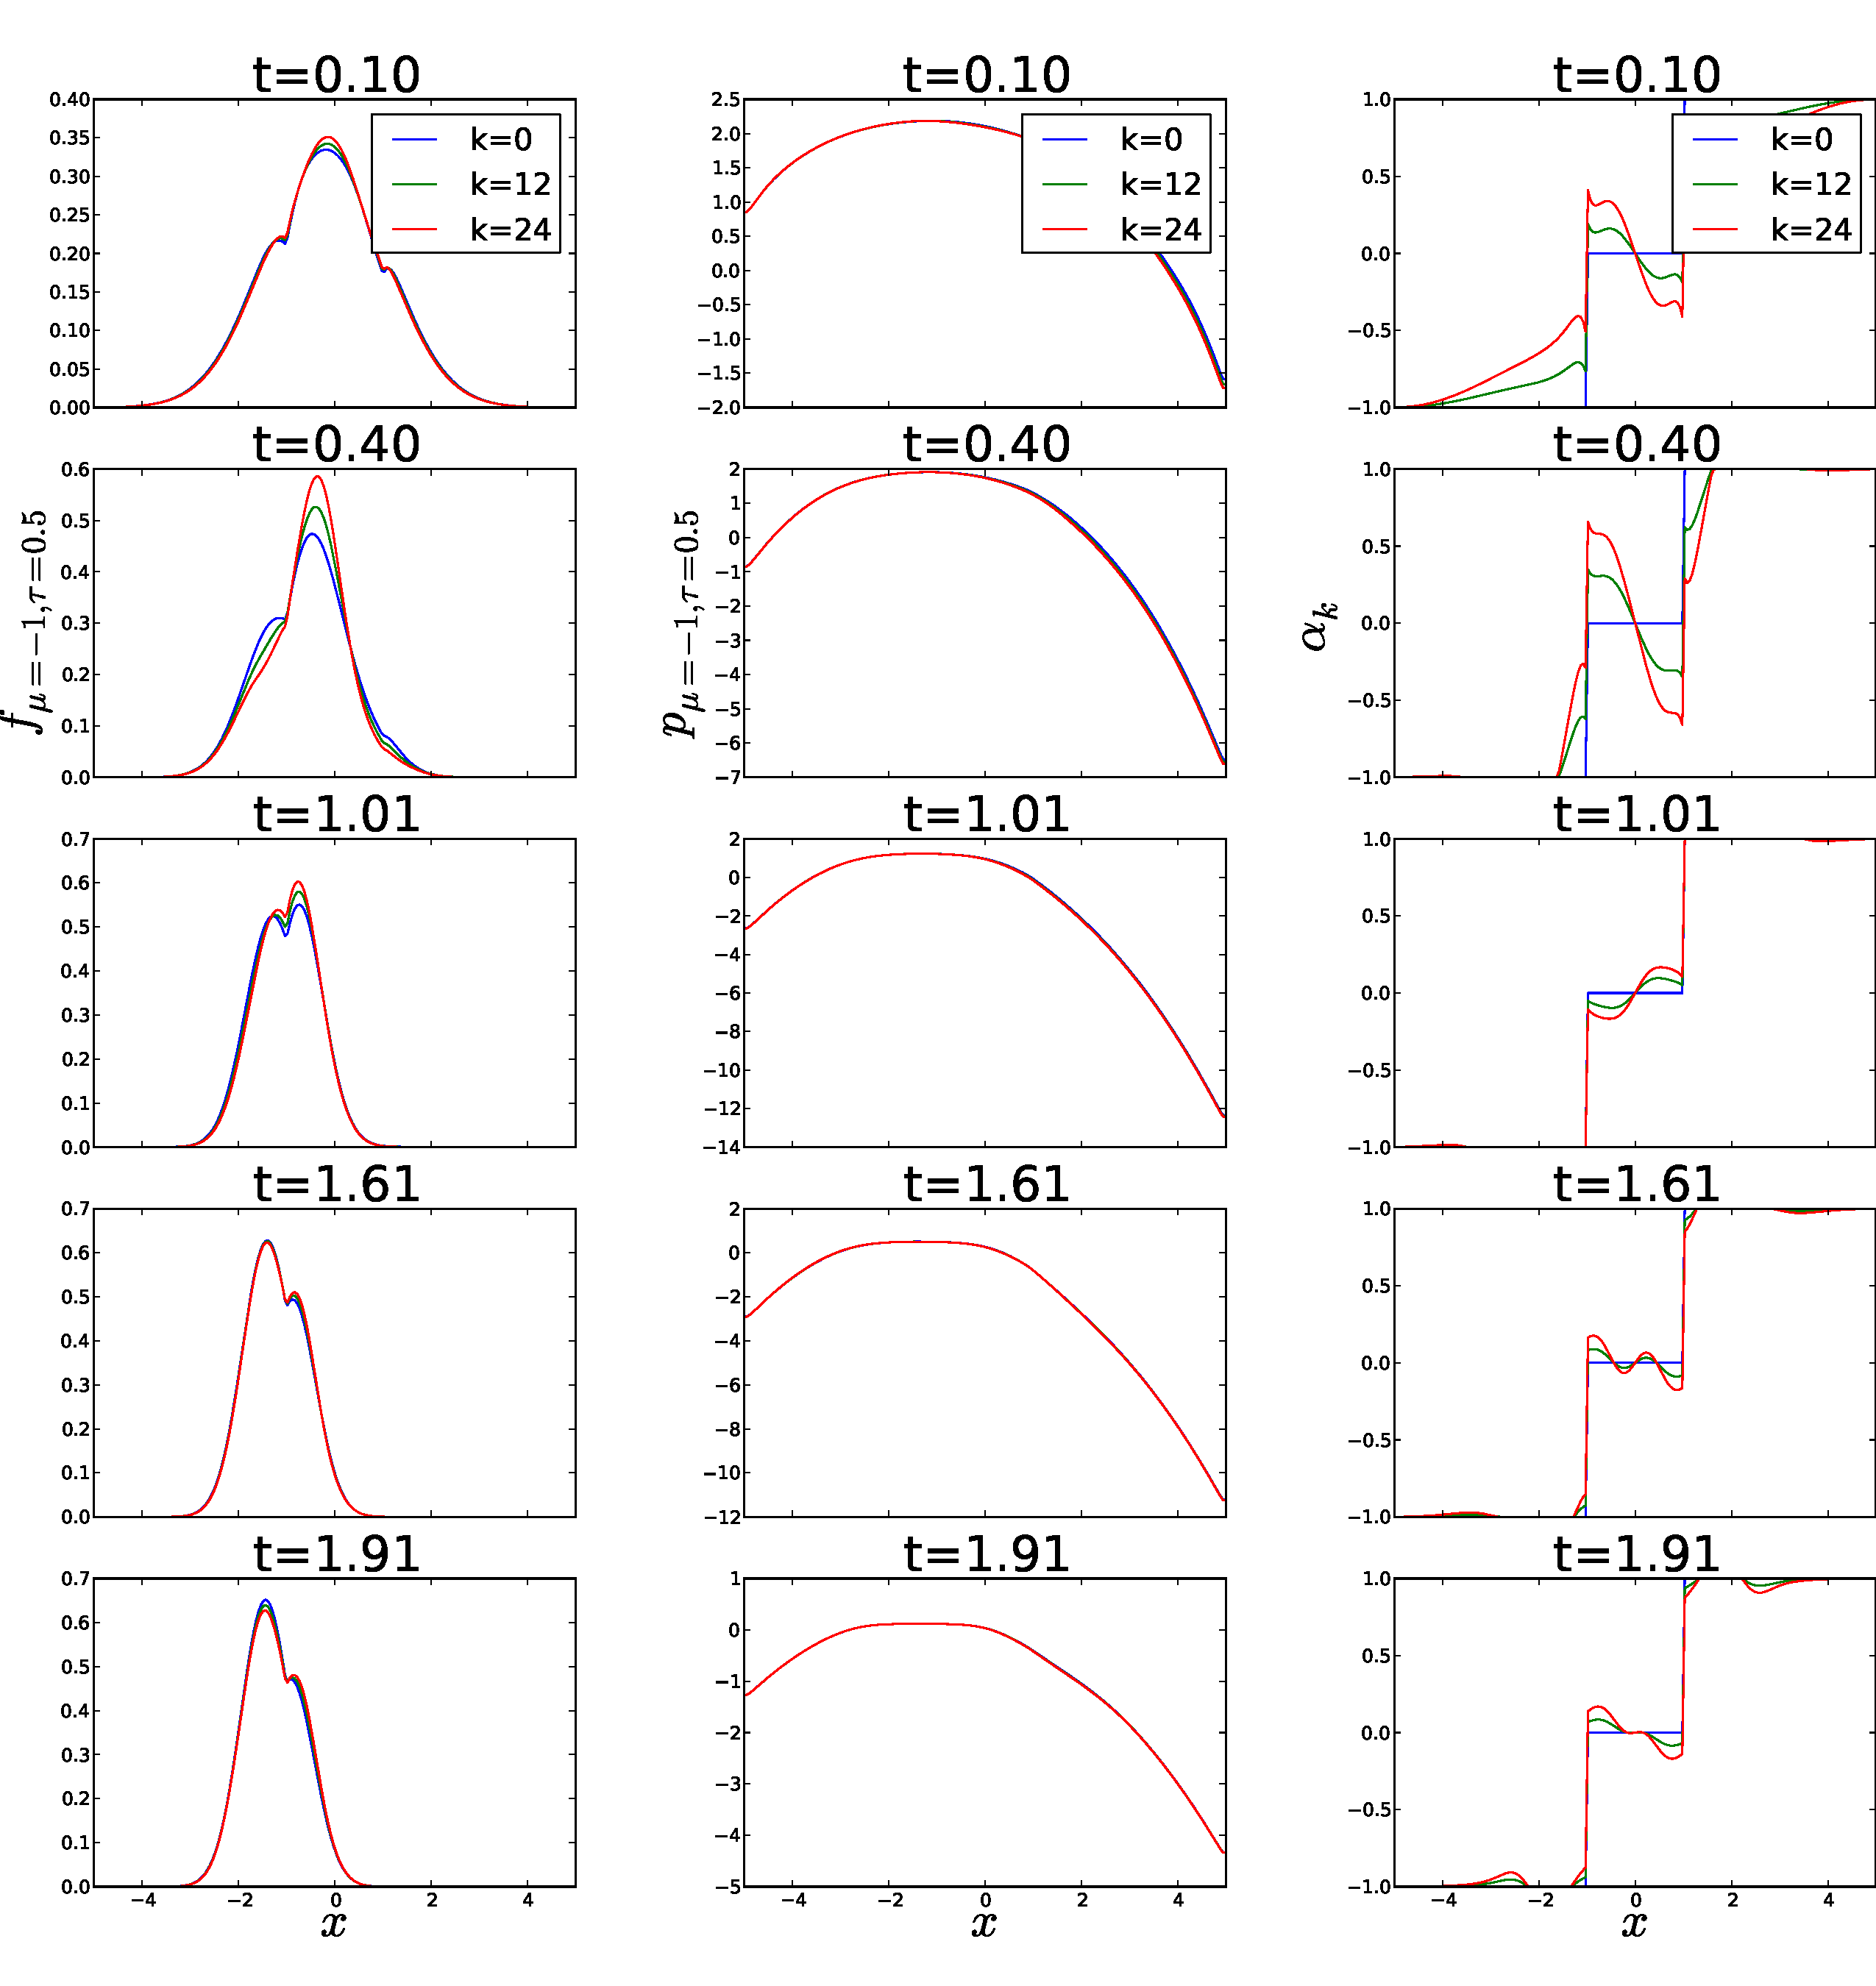
\includegraphics[width=1\textwidth]{Figs/OUFBSolver_BetaMu/FB_alpha_iterates_uICs_5_Tf=2.pdf}
  \caption[tableofCs]{The gradient ascent iterations for $f,p,\a$ when both
  $\tc, \m$ are uncertain. The initial guess for $\a_0$ is in 'blue' on the
  right-most }
  \label{fig:fpalpha_iterates_mubeta}
\end{center}
\end{figure}






\section{Problem Formulation}
The basic goal of 'Optimal Design' is to perturb a dynamical system in an
'optimal' way such as to 'best' estimate its structural parameters. 

As such the problem is a blend of optimal control and estimation, where the
objective of the optimal control is to improve the estimation, for example by
minimizing the variance of the estimators. 

For illustration sake we return to our favourite LIF model
Given a noisy LIF neuronal model:
\begin{equation}
\begin{gathered}
dX_s = (\underbrace{\a(t)}_{\textrm{control}} + \b(\m %\g \sin(\o t)
 - {X_s} ) \intd{s} + \s\intd{W_s},
\\
X(0) = .0,
\\
X(\ts) = \xth \implies  
\begin{cases}
X(\ts^+) &= .0   
\\
t_k &=  \ts
\\
k  &= k+1
\end{cases}
\end{gathered}
\label{eq:X_evolution_uo}
\end{equation}
where (a subset of) the parameter set $\th = \{\m, \b, \s\}$ is unknown.

Our goal is to choose $\a(t)$ as to estimate $\b$ 'best' given only that the
spike times $\{t_k\}$ are observed 
 
\section{Notation}
The probability density of the $n$th interval,
conditional on some applied control $\a$:
\begin{equation} 
\begin{array}{rcll} 
g_n(\t) \intd{\t} &:=& \Prob(I_{n} \in [\t, \t + \intd{\t})  \,|\,
 \a(t)) &
 \textrm{(probability density)} 
\\ 
G_{n}(t) &:=& \Prob \left[I_{n} \leq t  \,|\,
 \a(t) \right] = \int_0^t g_{\phi}(\t) \intd{\t} &
 \textrm{(cumulative distribution)}
\\
\G_{n}(t) &:= & \Prob(I_{n}>t \,|\, \a(t) ) = 1 - G_{\phi}(t)
&
 \textrm{(survivor distribution)}
\end{array}
\label{eq:ISI_distribution_functions}
\end{equation}
We'll drop the $n$ subscript when there is no confusion. 
There is also the transition distribution for $X_t$ for $t \in [0,
I_{n})$:
\begin{equation}
f(x,t) := \Prob \left[X_{t} \in x+ \intd{x}  \,|\,
 X_0 = 0, X_{s < t} < 1  \right]  \quad
 \textrm{(transition distribution)}
 \label{eq:transition_distribution}
\end{equation} 
\begin{equation}
\begin{gathered}
\begin{array}{lcl}
	\di_t f (x,t) &=&
					\underbrace{\frac{\b^2 }{2}}_{D}\cdot \di^2_x f 
					+ \di_x \Bigg(  
					\underbrace{\Big( \b (x-\m) - \a(t) \Big)}_{U(x,t)}  \cdot  f \Bigg)
					\\
					&=&
					D \cdot \di^2_x f +
					\di_x  \Big( U(x,t) \cdot f \Big)
					\\
					&=&
					- \di_x \phi(x,t)
					\\
					&=&
					\L[f] 
					\end{array}
	\\
	\left\{ \begin{array}{lcl}
	 f (x,0) &=& \delta(x)
	\\
	D \di_xf + U f |_{x=\xmin} &\equiv& 0 
	\\
	f |_{x=\xth} &\equiv& 0.
	\end{array} \right.
\label{eq:FP_pde_OU_absorbBC_CDF}
\end{gathered}
\end{equation}

The probability flux-out at the threshold boundary $$\phi(\xth, s) = D
\di_xf |_{x=\xth}$$ is very important as it is related to the spike-time density
via $$g( t)  = \phi(\xth, t) = D\cdot \di_x f|_{x=\xth}$$
 
% 
% In a typical (maximum likelihood) estimation experiment, we will see a lot of
% spikes and form the likelihood as
% $$
% L(\th| t_n ) = \prod_n g_n(t_n)
% $$
% We will then take logs and proceed as usual:
% $$
% l(\th| t_n ) = \sum_n \log (g_n(t_n)) =  \sum_n \log ( -\di_t F(1,t_n)) 
% $$
% and then maximize $l$ over the parameters $\th$. 
% 
% The associated {\sl score} function is
% $$
% S(\th | \ts ) = \grad_\th l(\th | \ts)
% $$
% The score function is a vector\footnote{We write $\grad$ for the vector
% differential and $\di$ for its scalar components, i.e.\ $\grad_\th =
% [\di_{\th_1},\ldots\di_{\th_i}],\ldots$}.
% 
% The typical Maximum Likelihood process is to 
% maximize the likelihood, $l$ which, if one uses a gradient-based approach
% amounts to finding the roots of the score, $S$.

In a Bayesian approach, we have some {\sl a priori} belief over the possible
values of $\th$.

Let us call the prior over the parameters $\th = \{\m, \b, \s\}$:
$$\rho(\th)$$.

Given a single observation $\ts$, the posterior of the parameter belief dist'n
is 
\begin{equation}
p(\th| \ts; \a) =
\frac{g(\ts |\th; \a)\cdot \rho(\th)}{\int_\Theta g(\ts|\th; \a)\cdot \rho(\th)
\intd{\th}}
\label{eq:parameter_posterior_defn}
\end{equation} 
Where $ g( \ts |\th; \a)$ is the likelihood of $X$ given in
\cref{eq:ISI_distribution_functions}.

The idea now, is to choose $\a$ such that the mutual information $I$ between the
two random variables is maximized. Here the Mutual Information is given by
\begin{equation}
I[\a]= 
\int_\Theta \int_{[0, \infty]} g(t|\th)\rho(\th) \cdot 
\log \left( \frac{g(t|\th)}
{\int_\Theta g(t|\th)\rho(\th) \intd{\th}   } \right)
\intd{t}\intd{\th}.
\label{eq:J_mutual_info_objective}
\end{equation}

See \cref{sec:mutual_info_defn} for why. 
Naturally for different controls, $\a(\cdot)$, the mutual info, $I$, will
be different since $g$, the hitting time density depends on the shape of $\a$.
($\rho$ does NOT).

However, there is an added complication b/c we actually will observe many
hitting times, and having less informative hitting times happen more often might
be better than hitting times which are informative but happen less often. 

The rigorous way to deal with this is to consider the mutual information between
the parameters and the set of hitting times $\{t_n\}$, however this seems
incredibly complicated, so instead we will maximize the 'Mutual Information
rate, $J$, which we define as 
\begin{align}
J[\a]= & \Exp[\ts]^{-1} \cdot I[\a]
\\
= & \frac{
\int_\Theta \int_{[0, \infty]} g(t|\th)  \rho(\th) \cdot 
\log \left( \frac{g(t|\th)}{\int_\Theta g(t|\th)\rho(\th) \intd{\th} } \right)
\intd{t}\intd{\th}}
{ \int_\Theta \int_{[0, \infty]} \t g(t|\th)\rho(\th) \intd{t}\intd{\th}}
\label{eq:J_mutual_info_rate_objective}
\end{align}

Well, this does NOT look any less complicated\ldots, Note that $g$ (and thus
implicitly $\a$) appears 4 times in this expression. Recall that $g$ is related
to $\a$ via the solution of the Fokker-Planck equation and thus we can also
write

\begin{align}
J[\a] 
= & \frac{
\int_\Theta \int_{[0, \infty]} \di_xf(1, t)  \rho(\th) \cdot 
\log \left( \frac{\di_xf(1, t)}{\int_\Theta \di_xf(1, t)\rho(\th) \intd{\th} } \right)
\intd{t}\intd{\th}}
{ \int_\Theta \int_{[0, \infty]} t \di_xf(1, t)\rho(\th) \intd{t}\intd{\th}}
\label{eq:J_mutual_info_rate_objective_in_terms_of_dixf} 
\end{align}
  
We want to find the control input $\a(t)$, which maximizes $J$ in
\cref{eq:J_mutual_info_rate_objective_in_terms_of_dixf}. 

\section{Gradient Ascent using Maximum Principle in order to maximize 
\cref{eq:J_mutual_info_rate_objective_in_terms_of_dixf} or rather the simpler 
\cref{eq:J_mutual_info_objective}} 

Let us discuss the optimization problem

$$
\a(\cdot) = \argmax_{\a \sim \textrm{admissible}} J[\a]
$$ 
   

\subsection{The nitty-grity of calculating the (infinite-dimensional) gradient
$\grad_{\a} J$ } We would like to maximize
\cref{eq:J_mutual_info_rate_objective_in_terms_of_dixf}, but now we realize that
doing so is very difficult, b/c we have a ratio of integrals. (The standard
theory always works with just one integral).

Let's then drop the denominator integral and focus on the numerator. (i.e. we
just go back to \cref{eq:J_mutual_info_objective})
\begin{equation}
I[\a] 
=  -
\int_\Theta \int_{[0, \infty]} \di_xf(1, t)  \rho(\th) \cdot 
\log \left( \frac{ \di_xf(1, t)}{\int_\Theta \di_xf(1, t)\rho(\th) \intd{\th}
} \right)
\intd{t}\intd{\th}
\label{eq:I_mutual_info_objective_in_terms_of_dixf} 
\end{equation}

To proceed, we apply a Maximum Principle type derivation, in which we first seek
the differential of the objective $I$ in
\cref{eq:I_mutual_info_objective_in_terms_of_dixf} wrt.\
$\a(\cdot)$ and proceed from there.   

As always, we start by augmenting our objective functional with the
dynamics:
\begin{align}
I=&  
\int_\Theta \int_{[0, \infty]} \di_xf_\th(1, t)  \rho(\th) \cdot 
\log \left( \frac{\di_xf_\th(1, t)}{\int_\Theta \di_xf_\th(1, t)\rho(\th)
\intd{\th} } \right)
\intd{t}\intd{\th} 
\\
	  &- \int_\Theta \int_0^\infty <p_\th, (\di_t f_\th - \L[f_\th])> \intd{s} 
\end{align}
where the inner product, $<f, g>$ is just the space integral $\int f\cdot g
\intd{x}$ and we write $\L$ for the spatial differential operator in 
\cref{eq:FP_pde_OU_absorbBC_CDF}.

This is exactly the same problem as we faced in the spike-time optimal control,
except there the integrand looked something like $(t-t^*)D\di_xf$. Thus the
equations for the adjoint look exactly the same as there, with the exception of the Terminal
Conditions (here assumed 0) and the BCs at the threshold:



In short, the equation for the adjoint function, $p$, is
\begin{equation}
\begin{gathered}
\begin{aligned}
\di_t p =& - \Lstar[p]
\\
		=&
			- \Big[ D\cdot \di^2_x p +
			 U(x,t,\th)   \cdot \di_x p \Big].
\end{aligned}
\\
\begin{cases}
	p_\th \big|_{x=\xth} &=  \log\left(\frac{\di_xf_\th}{\int_\Th
	\di_xf_\th \rho(\th)\intd{\th})}\right) +
	 1 -
	  \frac{\di_xf_\th}{\int_\Th
	\di_xf_\th \rho(\th)\intd{\th})}
	\\
	\di_x p_\th  \big|_{x=\xmin} &= 0
	\\
	p_\th(x,\infty) &= 0
\end{cases}
\label{eq:adjoint_pde_OU}
\end{gathered}
\end{equation}

In practice of-course, we will set the terminal conditions for $p_\th$ at some
finite value of $t$

\vskip10pt The whole goal of this exercise is to calculate the differential of
$I$ in \cref{eq:I_mutual_info_objective_in_terms_of_dixf},
wrt.\ the control $\a(t)$, i.e.\ to calculate $\delta I / \delta \a$. After the
introduction of the adjoint state, $p_\th$, that is just:

 
\begin{align*}
\delta I =&   
\int_\Theta  \rho(\th) \cdot \Bigg(  
- \int_\xmin^{1} \di_x p_\th f_\th \intd{x} + 
   p_\th f_\th \Big|_\xmin 
    \Bigg) \intd{\th}
\end{align*}

I.e for a given $\alpha(t)$, we solve for $p,f$ and a few values of $\th$ from
the current belief distribution $\rho(\th)$ and their corresponding
probabilities/weights. Compute the above expression and increment $\alpha$ in
the direction of increasing $\delta I$.

In practice, we usually take a very simple prior, something like three values
with equal probability, something like:.
\begin{equation}
\rho(\b) = 
\begin{cases}
	\tfrac 13 & \textrm{if } \b= \in \{.5,    1 ,  2 \}\\
	0   &\textrm{o/w }
\end{cases}
\label{eq:basic_prior_over_tau}
\end{equation} 

\subsection{Effect of the Prior}

Here we show that the optimal control is sensitive to the {\sl spread} of the
prior, for example if we have a tightly clustered vs. loosely spread prior, both
centred at roughly the same mean (the log-prior has the same mean). 

Very interestingly, we see that while for a wide prior, the optimal control has
its characteristic double hump shape, that we have seen already, for a tight
prior, that is no longer the case

Thus we see that the shape of the prior {\sl has!}
an effect on the optimal control.

\begin{figure}[h]
\begin{center}
\subfloat[Wide Prior]
{
\label{fig:prior_spread_wide}
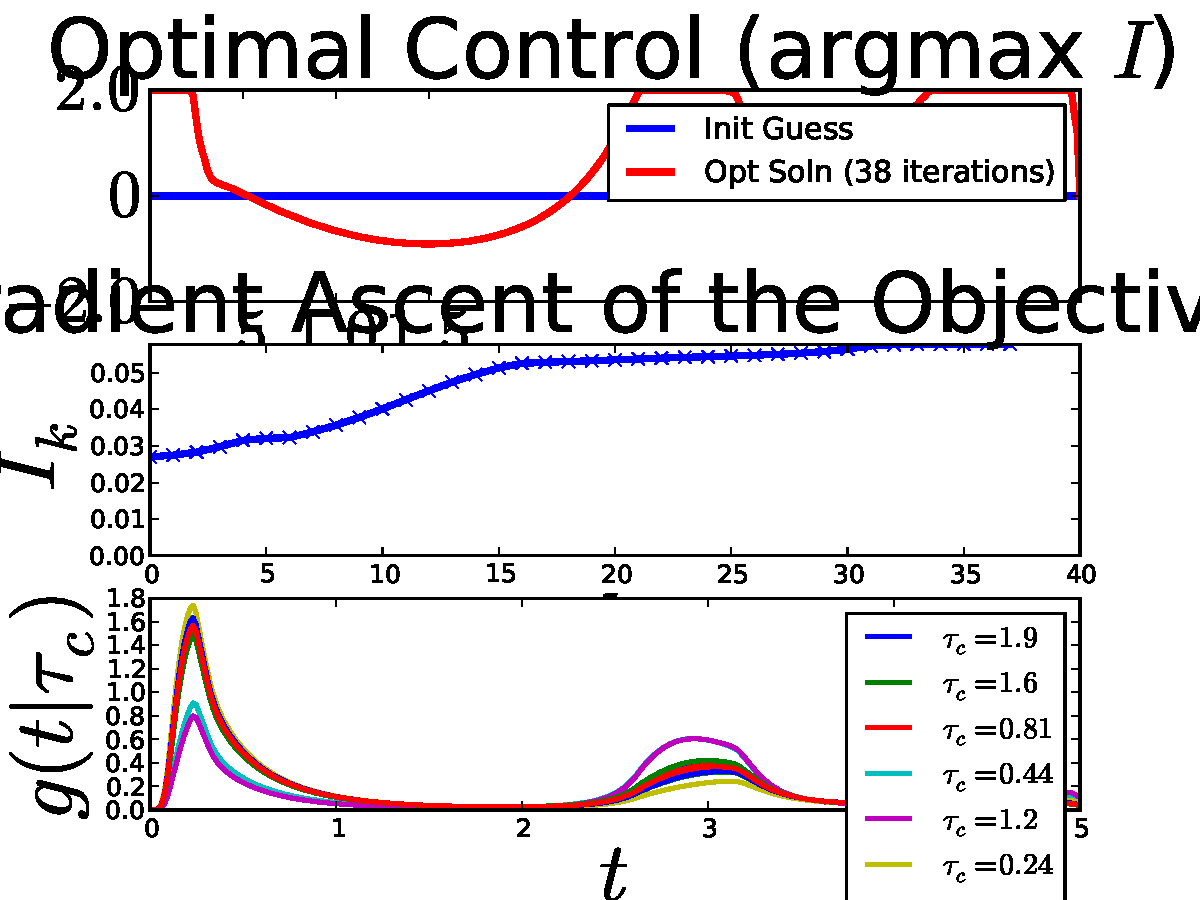
\includegraphics[width=0.48\textwidth]
{Figs/FP_Adjoint/PriorBox_wide_prior.pdf}
}
\subfloat[Tight Prior]
{
\label{fig:prior_spread_tight}
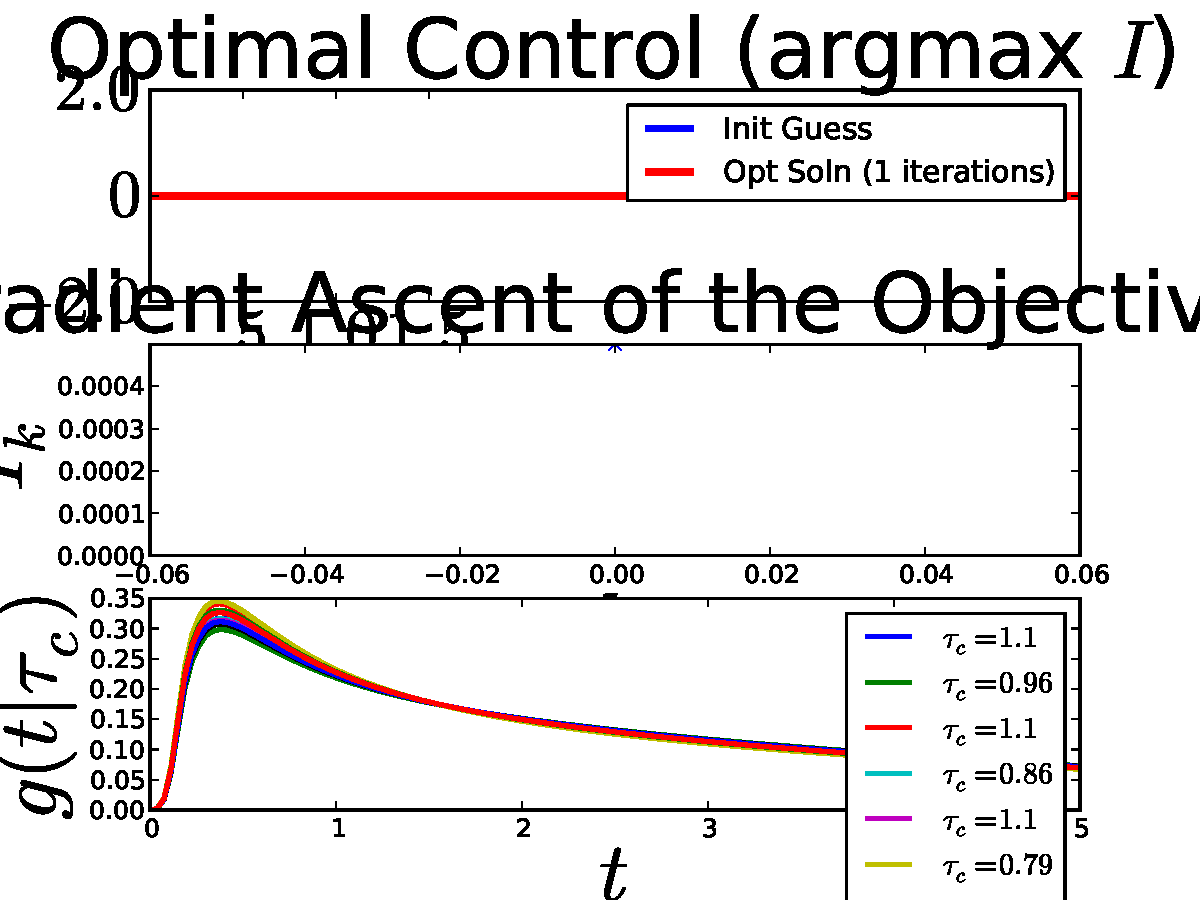
\includegraphics[width=0.48\textwidth]
{Figs/FP_Adjoint/PriorBox_concentrated_prior.pdf}
}
\caption[labelInTOC]{The effect of the spread (variance) of the prior on the
resulting optimal control}
\label{fig:prior_spread}
\end{center}
\end{figure}

Let's look at it another way, we will consider our basic prior as a function of
$w$
\begin{equation}
\rho(\b) = 
\begin{cases}
	\tfrac 12 & \textrm{if } \b= \in \{1- w, 1/(1-w) \}\\
	0   &\textrm{o/w }
\end{cases} 
\end{equation} 
and sweep for $w = .1:.1:.9$ (in matlab notation).

The results are in \cref{fig:effect_of_prior_width}. Looking at
\cref{fig:effect_of_prior_width}, we might be optimistic to hypothesize that we
should be doing this online and as the uncertainty (roughly speaking $w$) of the
parameter decreases, we should be changing the applied control\ldots This
brings us to {\sl adaptive } versions of our scheme which is NOT something we
have yet implemented. 
 
\begin{figure}[h]
\begin{center} 
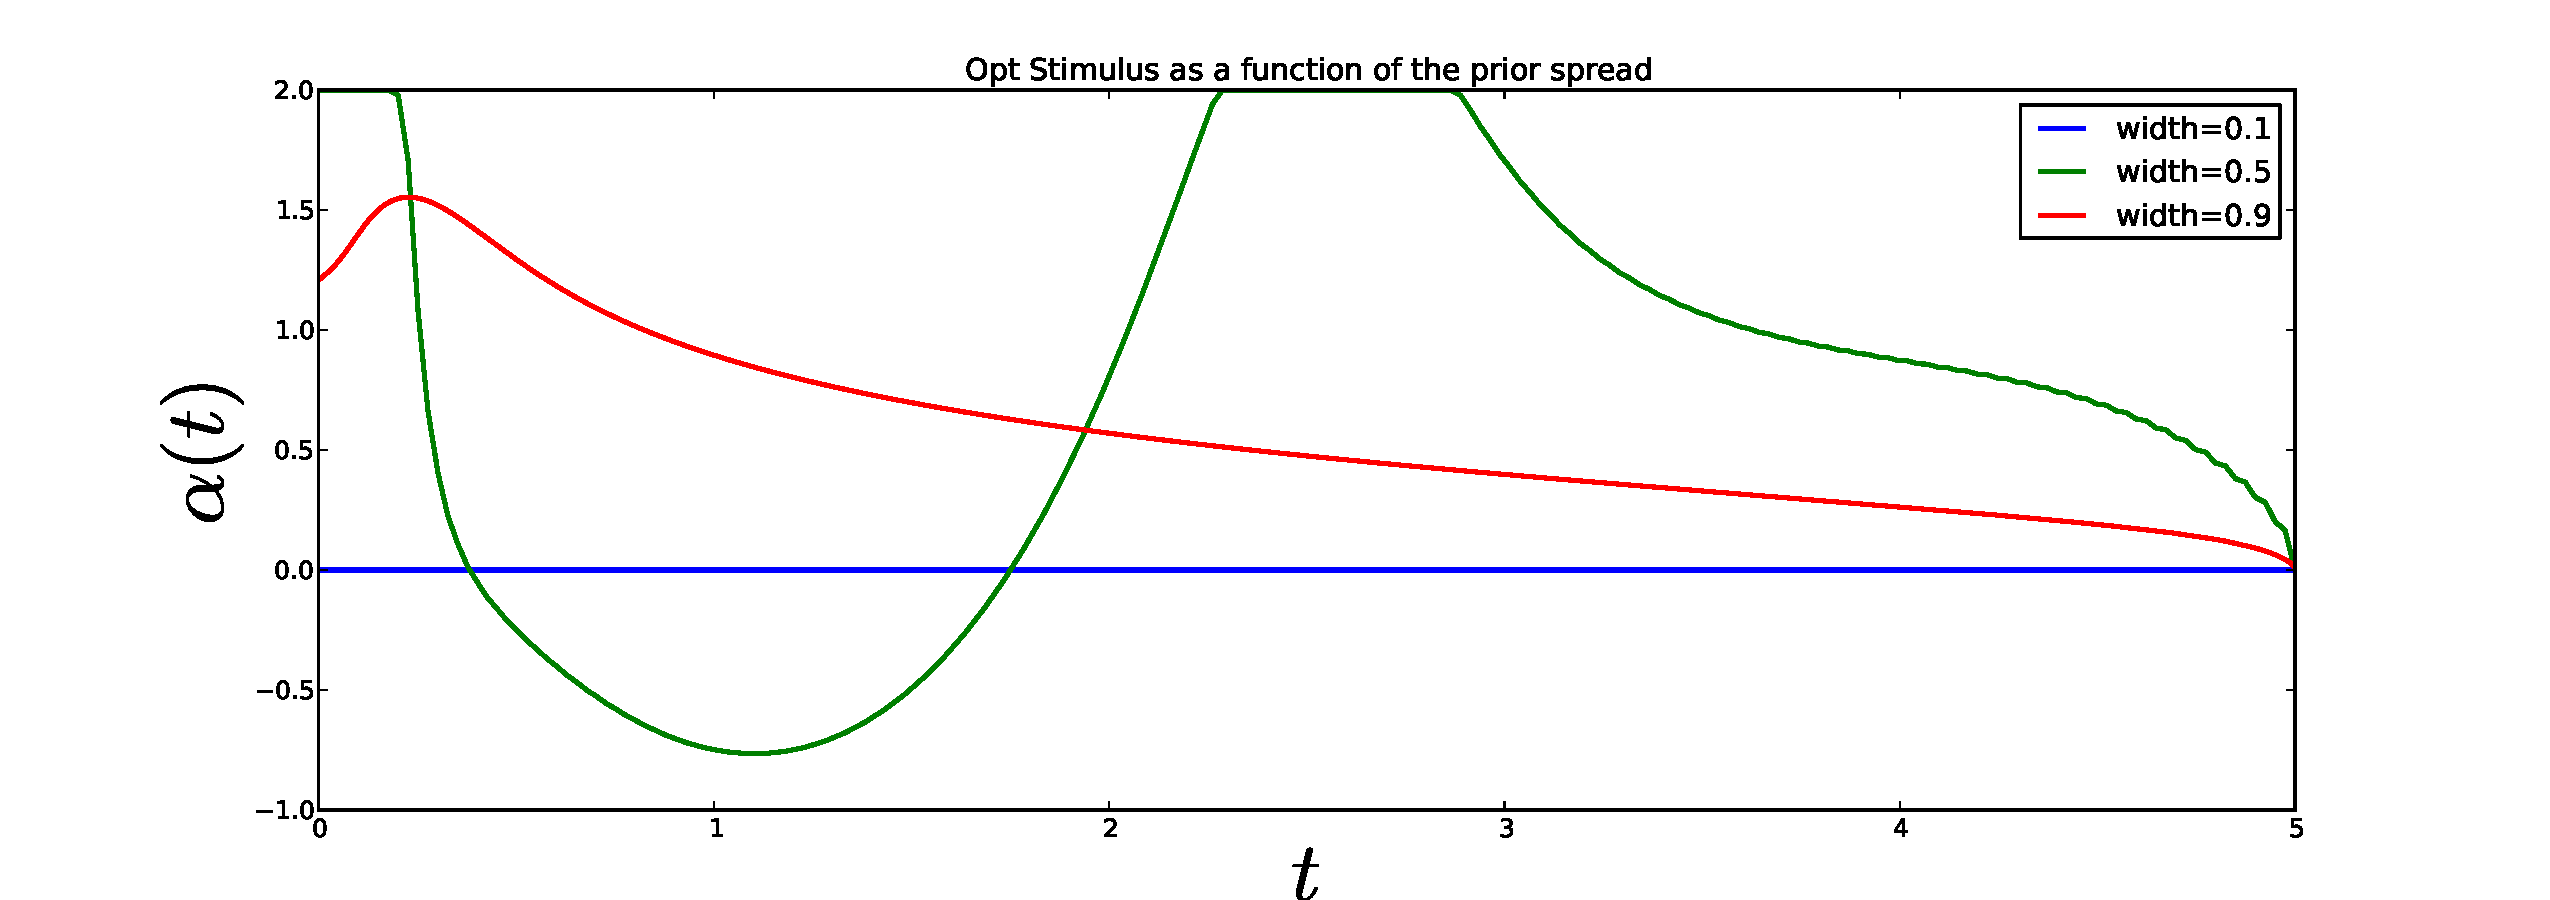
\includegraphics[width=\textwidth]
{Figs/FP_Adjoint/Effect_of_prior_spread.pdf} 
\caption[labelInTOC]{The effect of the width ($w$, a measure
of uncertainty) of the prior on the resulting optimal control}
\label{fig:effect_of_prior_width}
\end{center}
\end{figure}


\clearpage
\section{Basic Estimation Experiment}

We will run the following test:

Assume the true parameters
$$
 \m = 0; \b = 1; \s = 1.;
$$
We will assume we know $\s, \m$ and don't know $\b$ so we are trying to
maximize the Mutual Information between $\ts$ and $\b$.
 
Let's assume a very simple uniform prior on $\b$, $\b_i = \{.5, 1. 2\},$
each with probability 1/3. 

Then running the gradient ascent (details of the gradient ascent are omitted) we
get the controls, objective and hitting time densities shown in 
\cref{fig:hitting_time_density_g_aopt_bprior}. The optimal control seems to be
independent of the # of pts in the prior (i.e. instead of 3 we could use 5 pts
with weight 1/5 and get the same opt. control as in
\cref{fig:hitting_time_density_g_aopt_bprior}).



\begin{figure}[htp] 
\begin{center}
  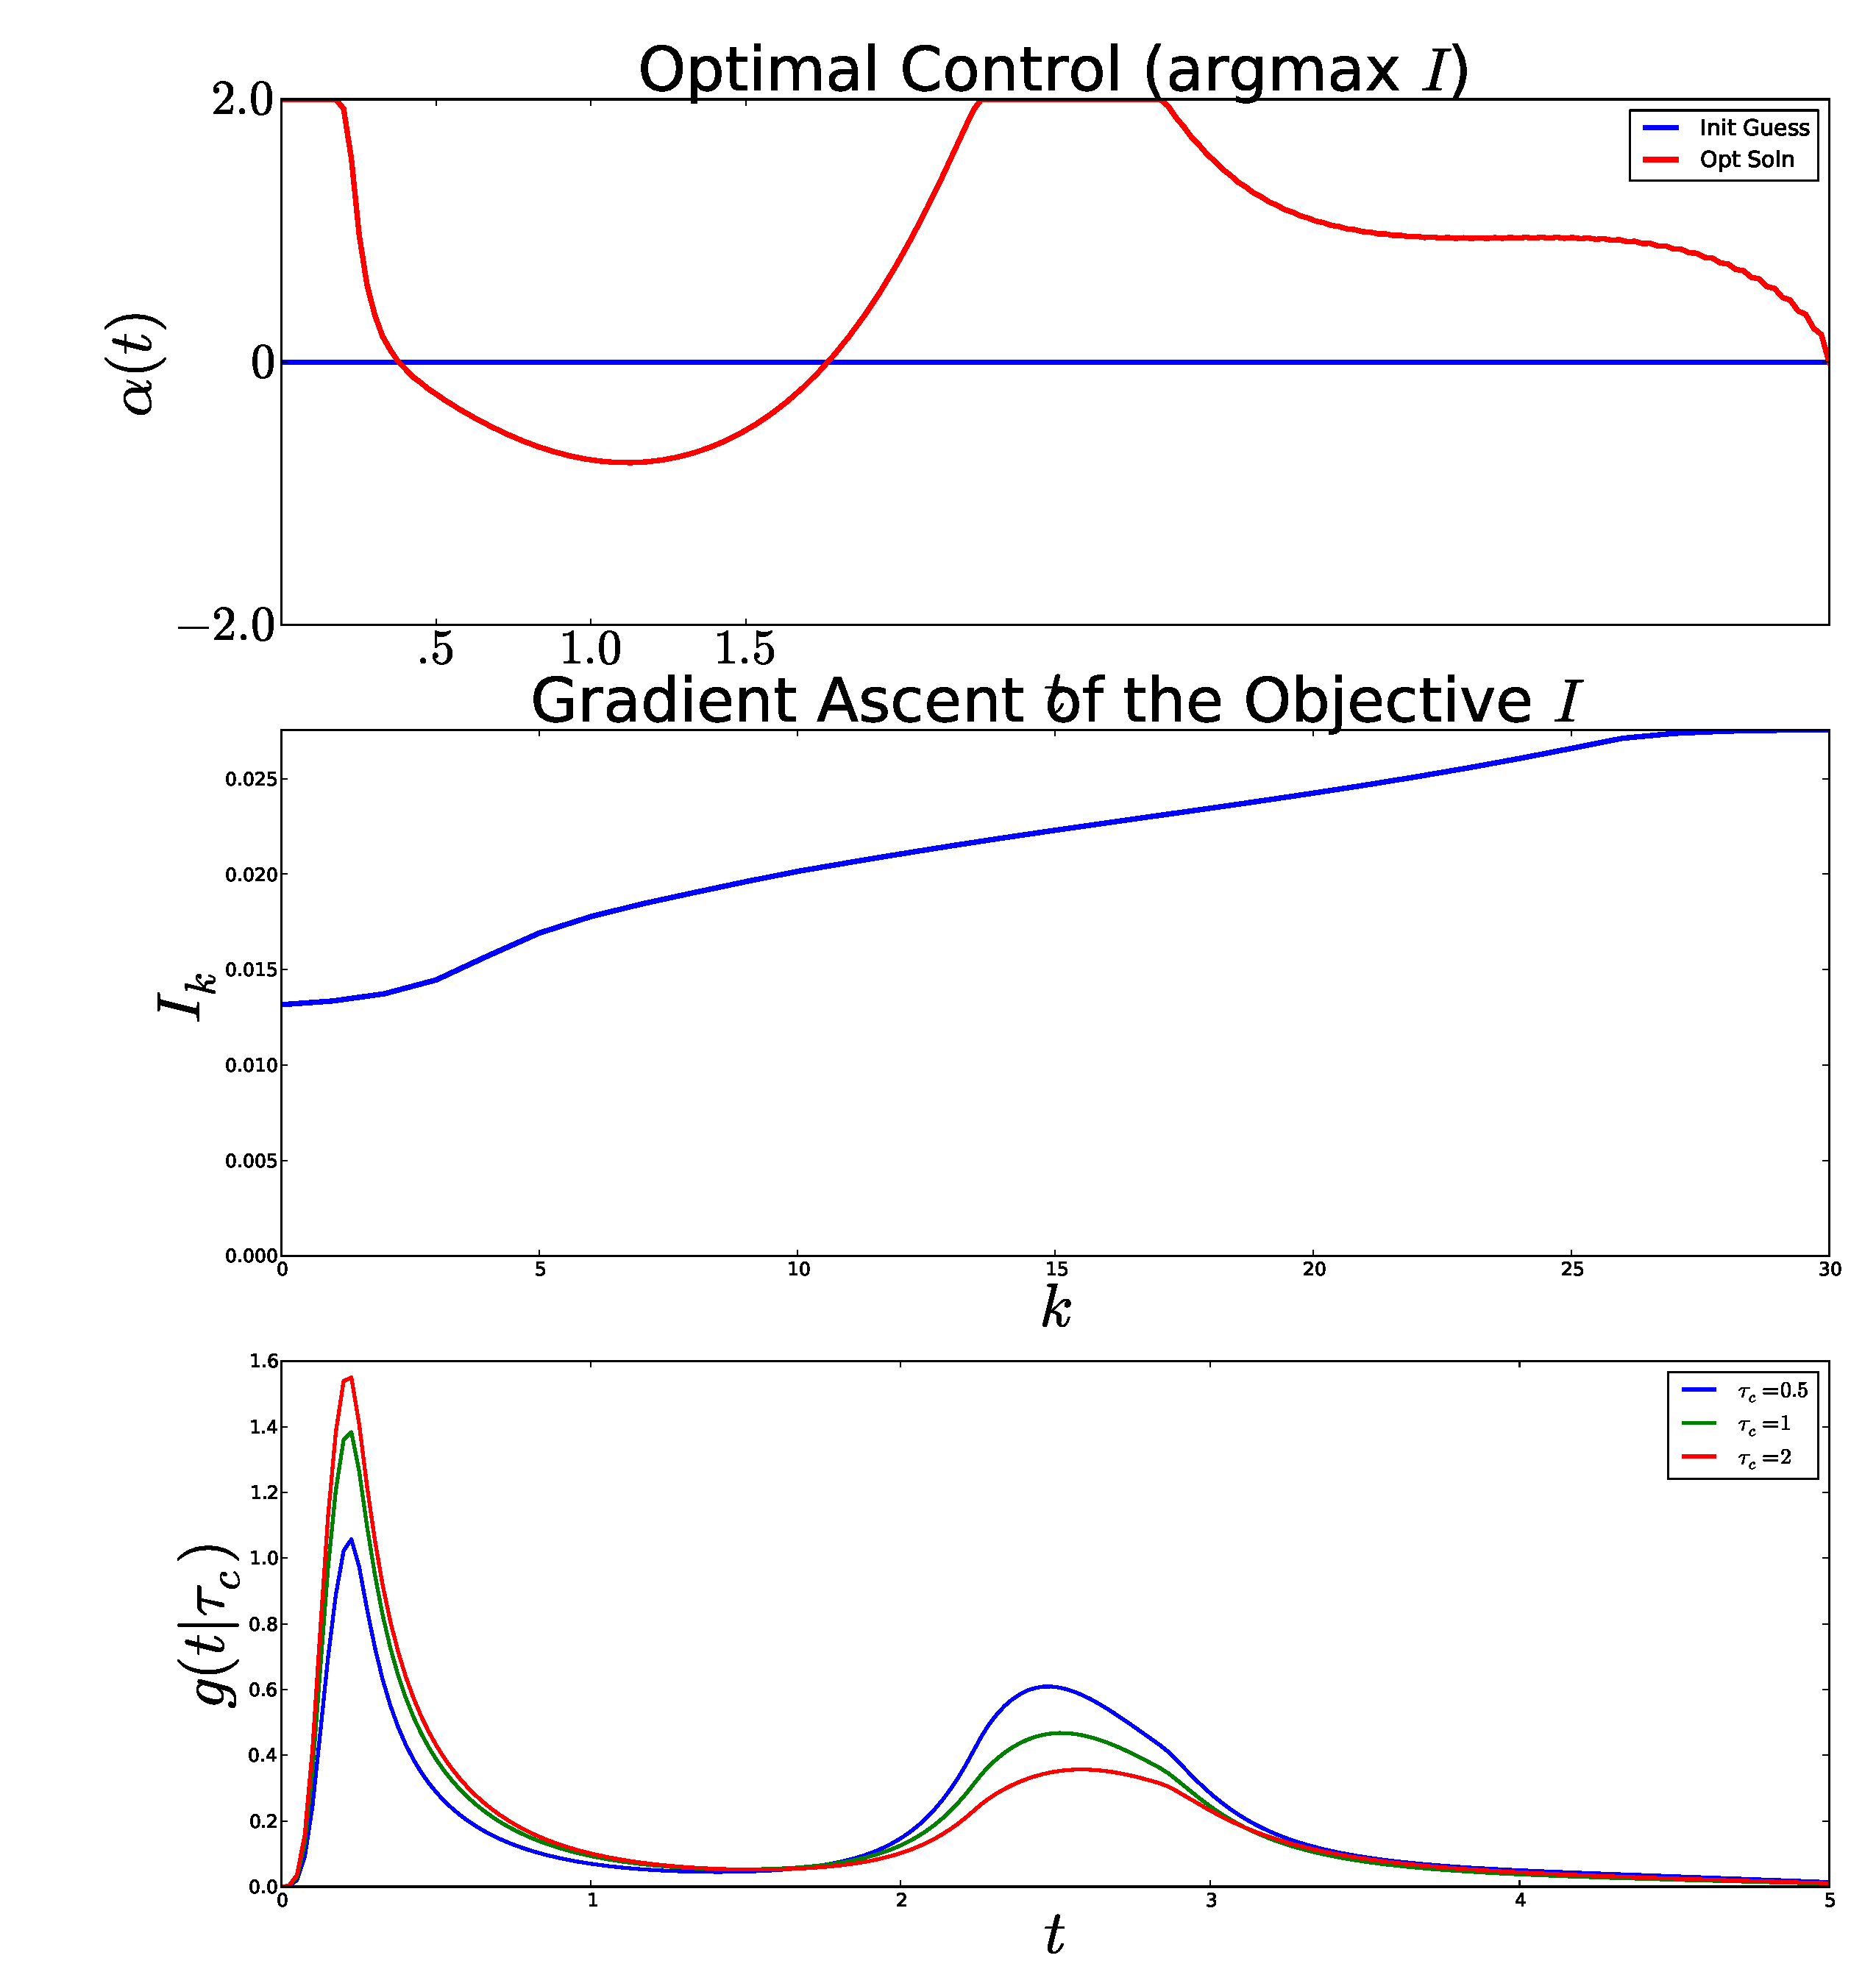
\includegraphics[width=1\textwidth]{Figs/FP_Adjoint/ExampleOptControl_MI_HT.pdf}
  \caption[labelInTOC]{The gradient ascent for the optimization of $I$ in
  \cref{eq:I_mutual_info_objective_in_terms_of_dixf}. Top panel, the initial and
  the optimal optimal controls, $\a_{0}(t), \a_{opt}(t)$
   true' density $
  g_{\a}(s|\b = 1.)$, ) given various controls (top panel) and the resulting Mutual Information ($I$ ) i.e using \cref{eq:J_mutual_info_objective} NOT \cref{eq:J_mutual_info_rate_objective}.
  The bottom plot shows the hitting times $g(t| \tc)$ corresponding to the 3
  distinct values of $\tc$ in the prior $\rho(\tc)$}
  \label{fig:hitting_time_density_g_aopt_bprior}  
\end{center}
\end{figure} 

\subsubsection{Aside: the nitty-gritty of the estimation procedure}
We have posed a fairly-simple estimation objective, in that it amounts to single
variable optimization. The negative log-likelihood of an observed hitting-time
set $\{t_n\}$ is
\begin{equation}
l(\b) = - \sum_n \log ( g(t_n | \b) ) =  - \sum_n \log ( -D \di_x f(t_n |
\b) |_{\xth} )
\end{equation}

The distributions are exemplified in
\cref{fig:log_likelihood_beta_examples_1000,fig:log_likelihood_beta_examples_10000,fig:log_likelihood_beta_examples_100000},
for three different values of $N_s = 1e3, 1e4, 1e5$ respectively. We see that in
principle it is very hard to distinguish between different values of $\b$. In
\cref{fig:log_likelihood_beta_examples_10000}, we see the first indications that
the Opt Control, might have some superiority over the 'Crit' Control (for
example) as it seems to estimate a $\b$ closer to 1 (the 'true' value). However,
on average, the different shapes of $\a(t)$ seems to have a very limited impact
on the estimates for $\b$ (even though it has a very obvious impact on the shape
of the hitting time dist'n $g(t)$).


\begin{figure}[h]
\begin{center} 
\subfloat[opt]  
{
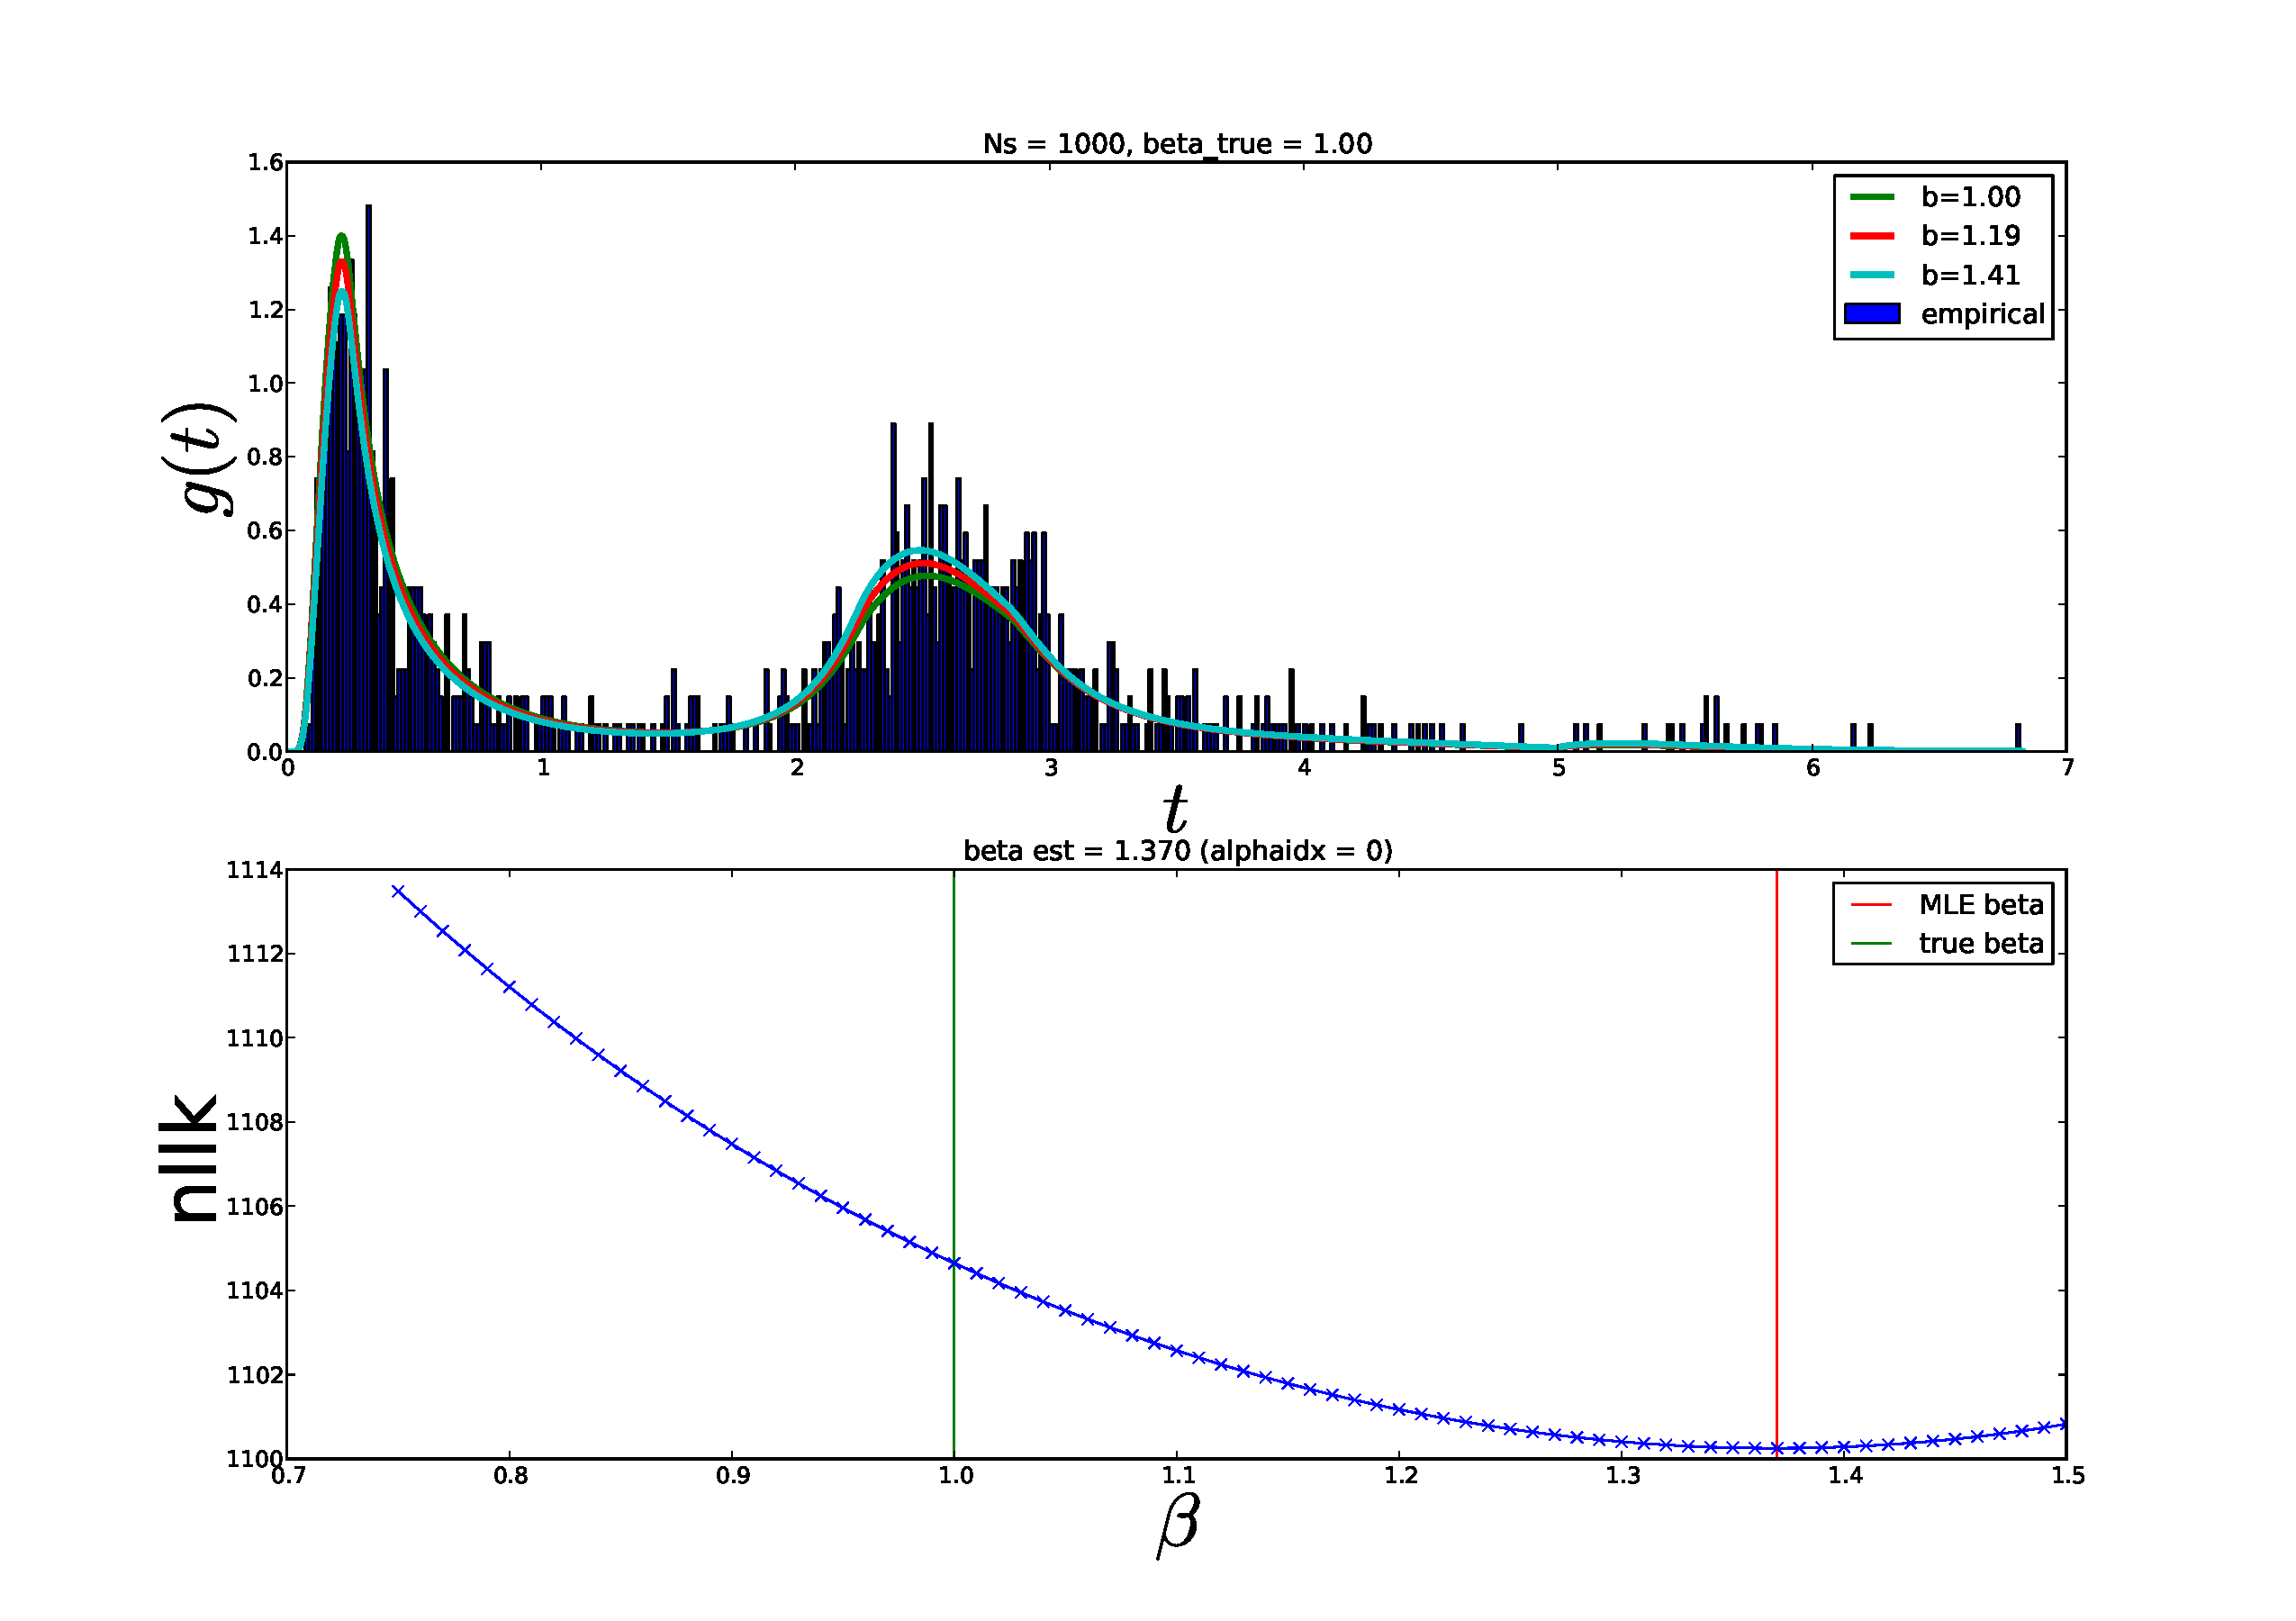
\includegraphics[width=.75\textwidth]
{Figs/HitTime_MI_TauChar_Adjoint_Estimate/Adjoint_TauChar_Estimator_estimatorWorkbench_b=0x1000_a0.pdf}
}
\\   
\subfloat[crit]
{
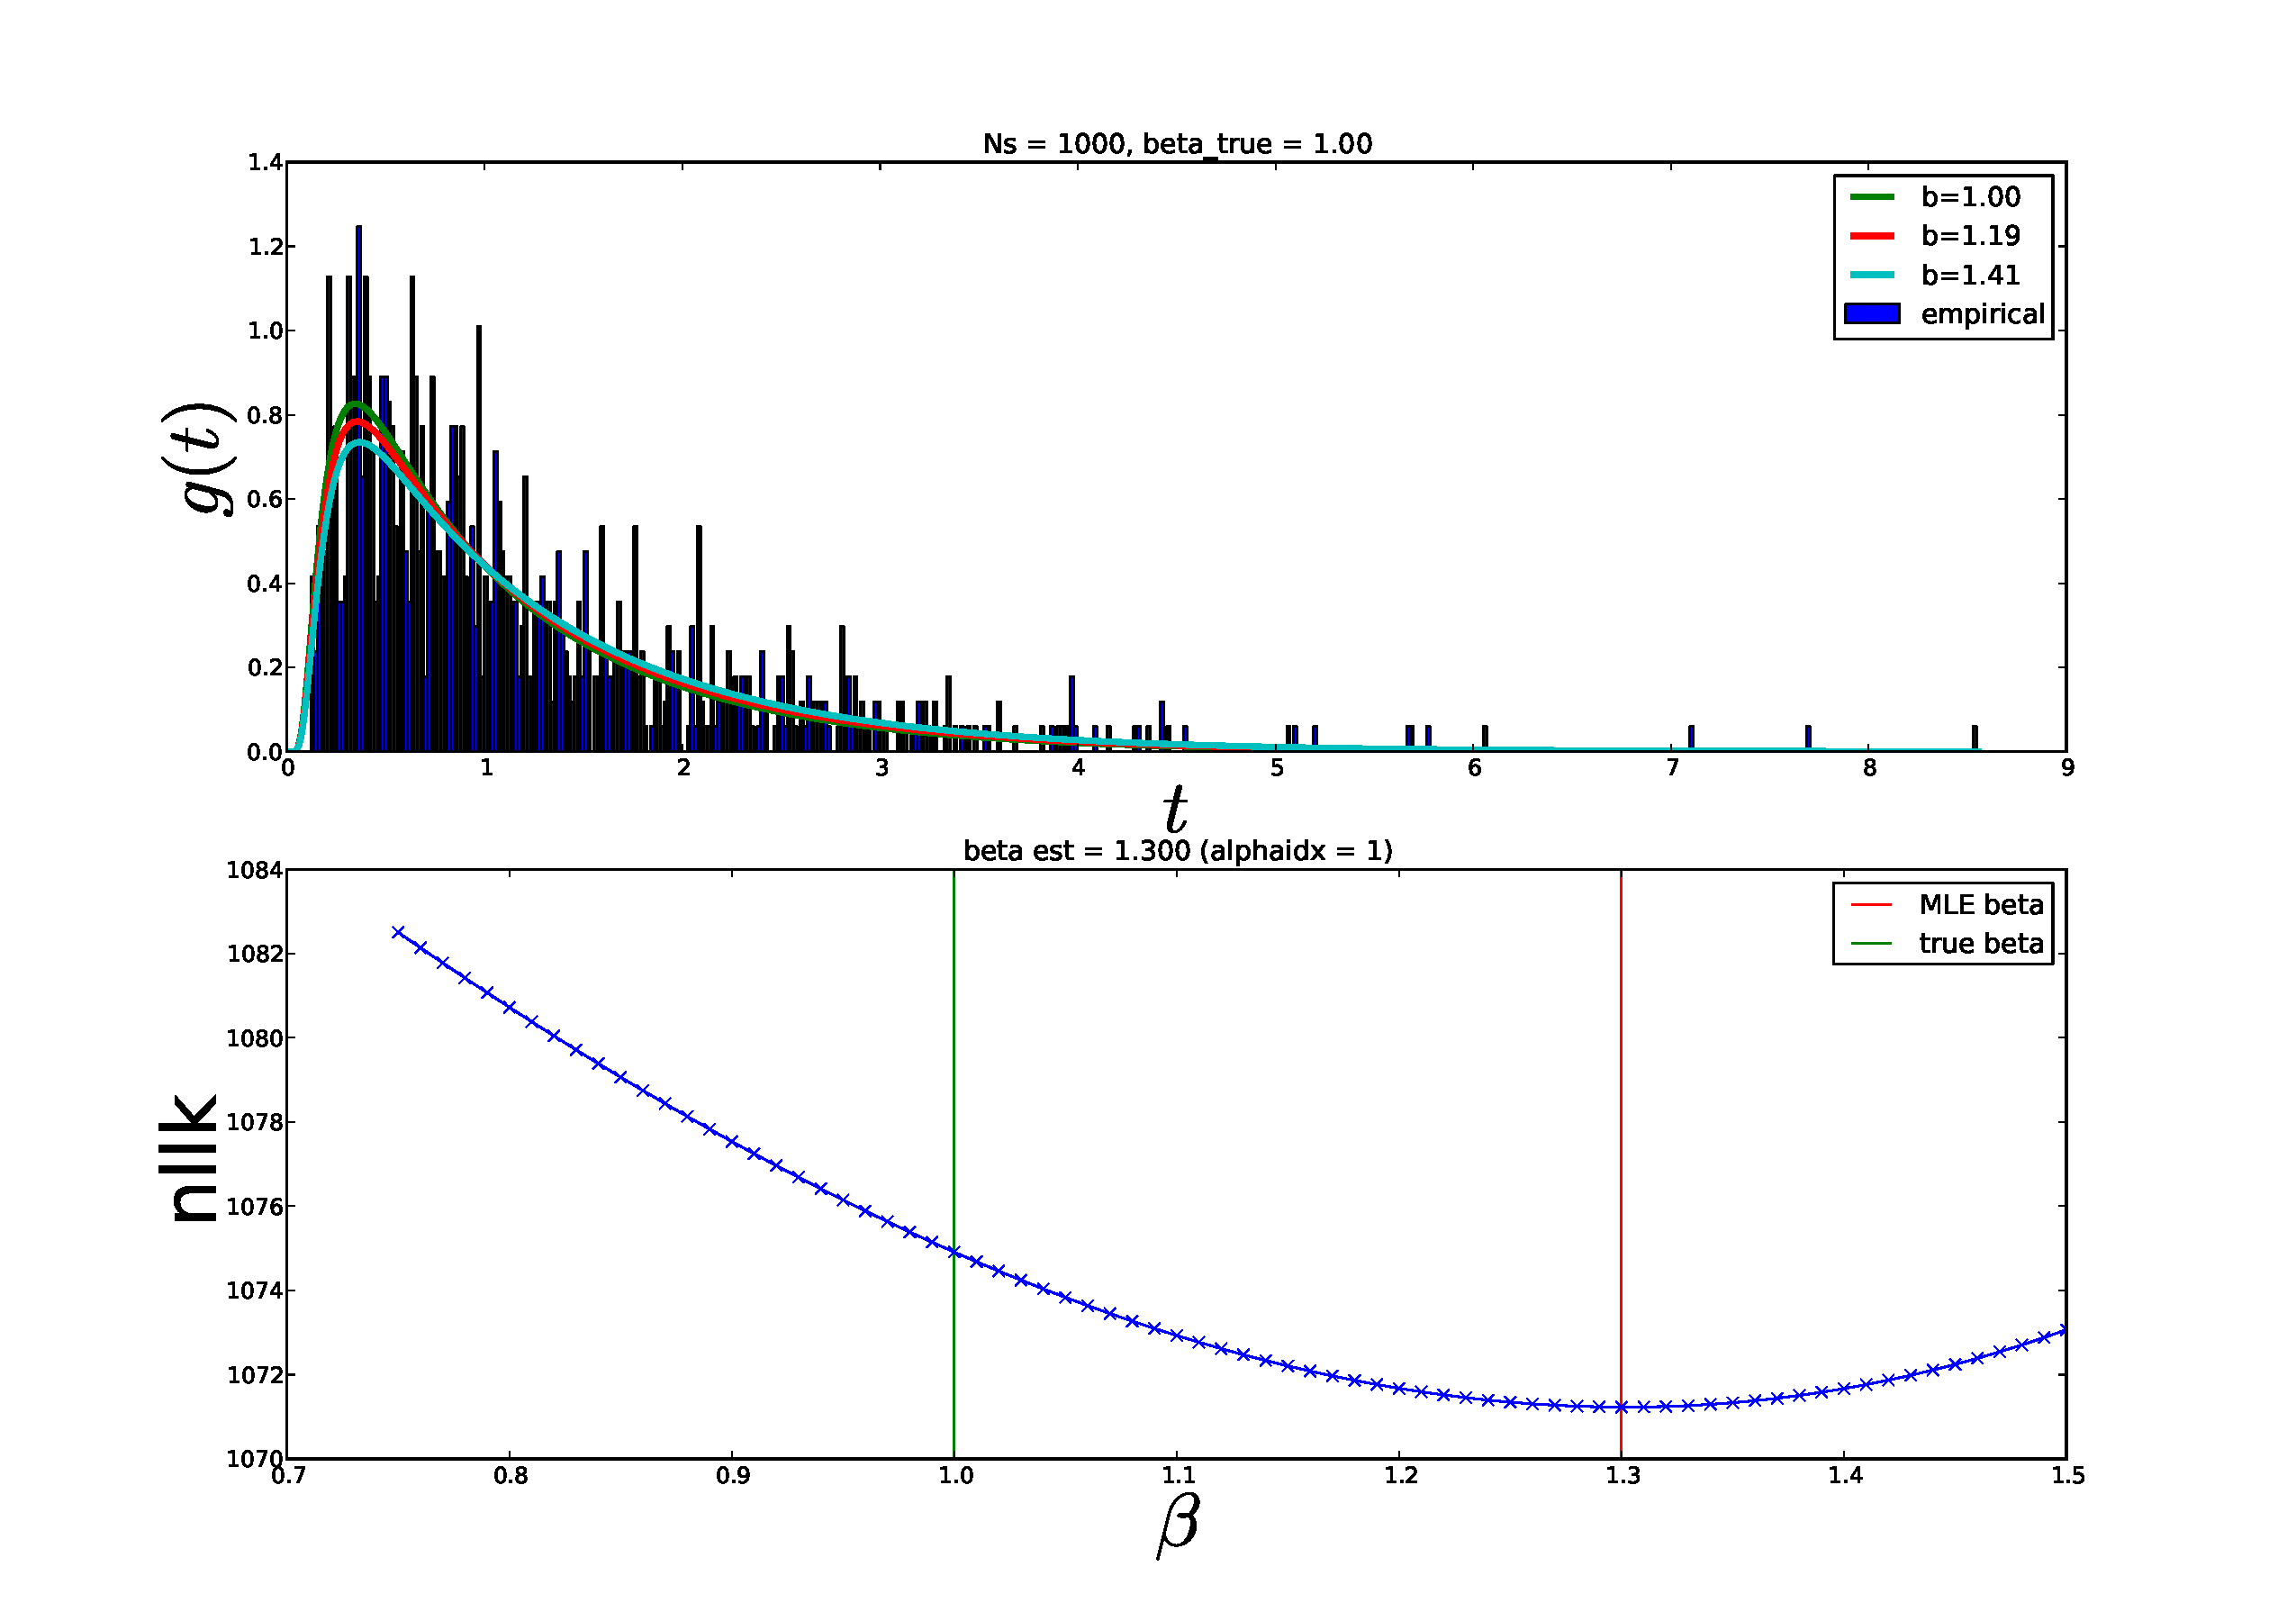
\includegraphics[width=.75\textwidth]
{Figs/HitTime_MI_TauChar_Adjoint_Estimate/Adjoint_TauChar_Estimator_estimatorWorkbench_b=0x1000_a1.pdf}
}
\\
\subfloat[max] 
{
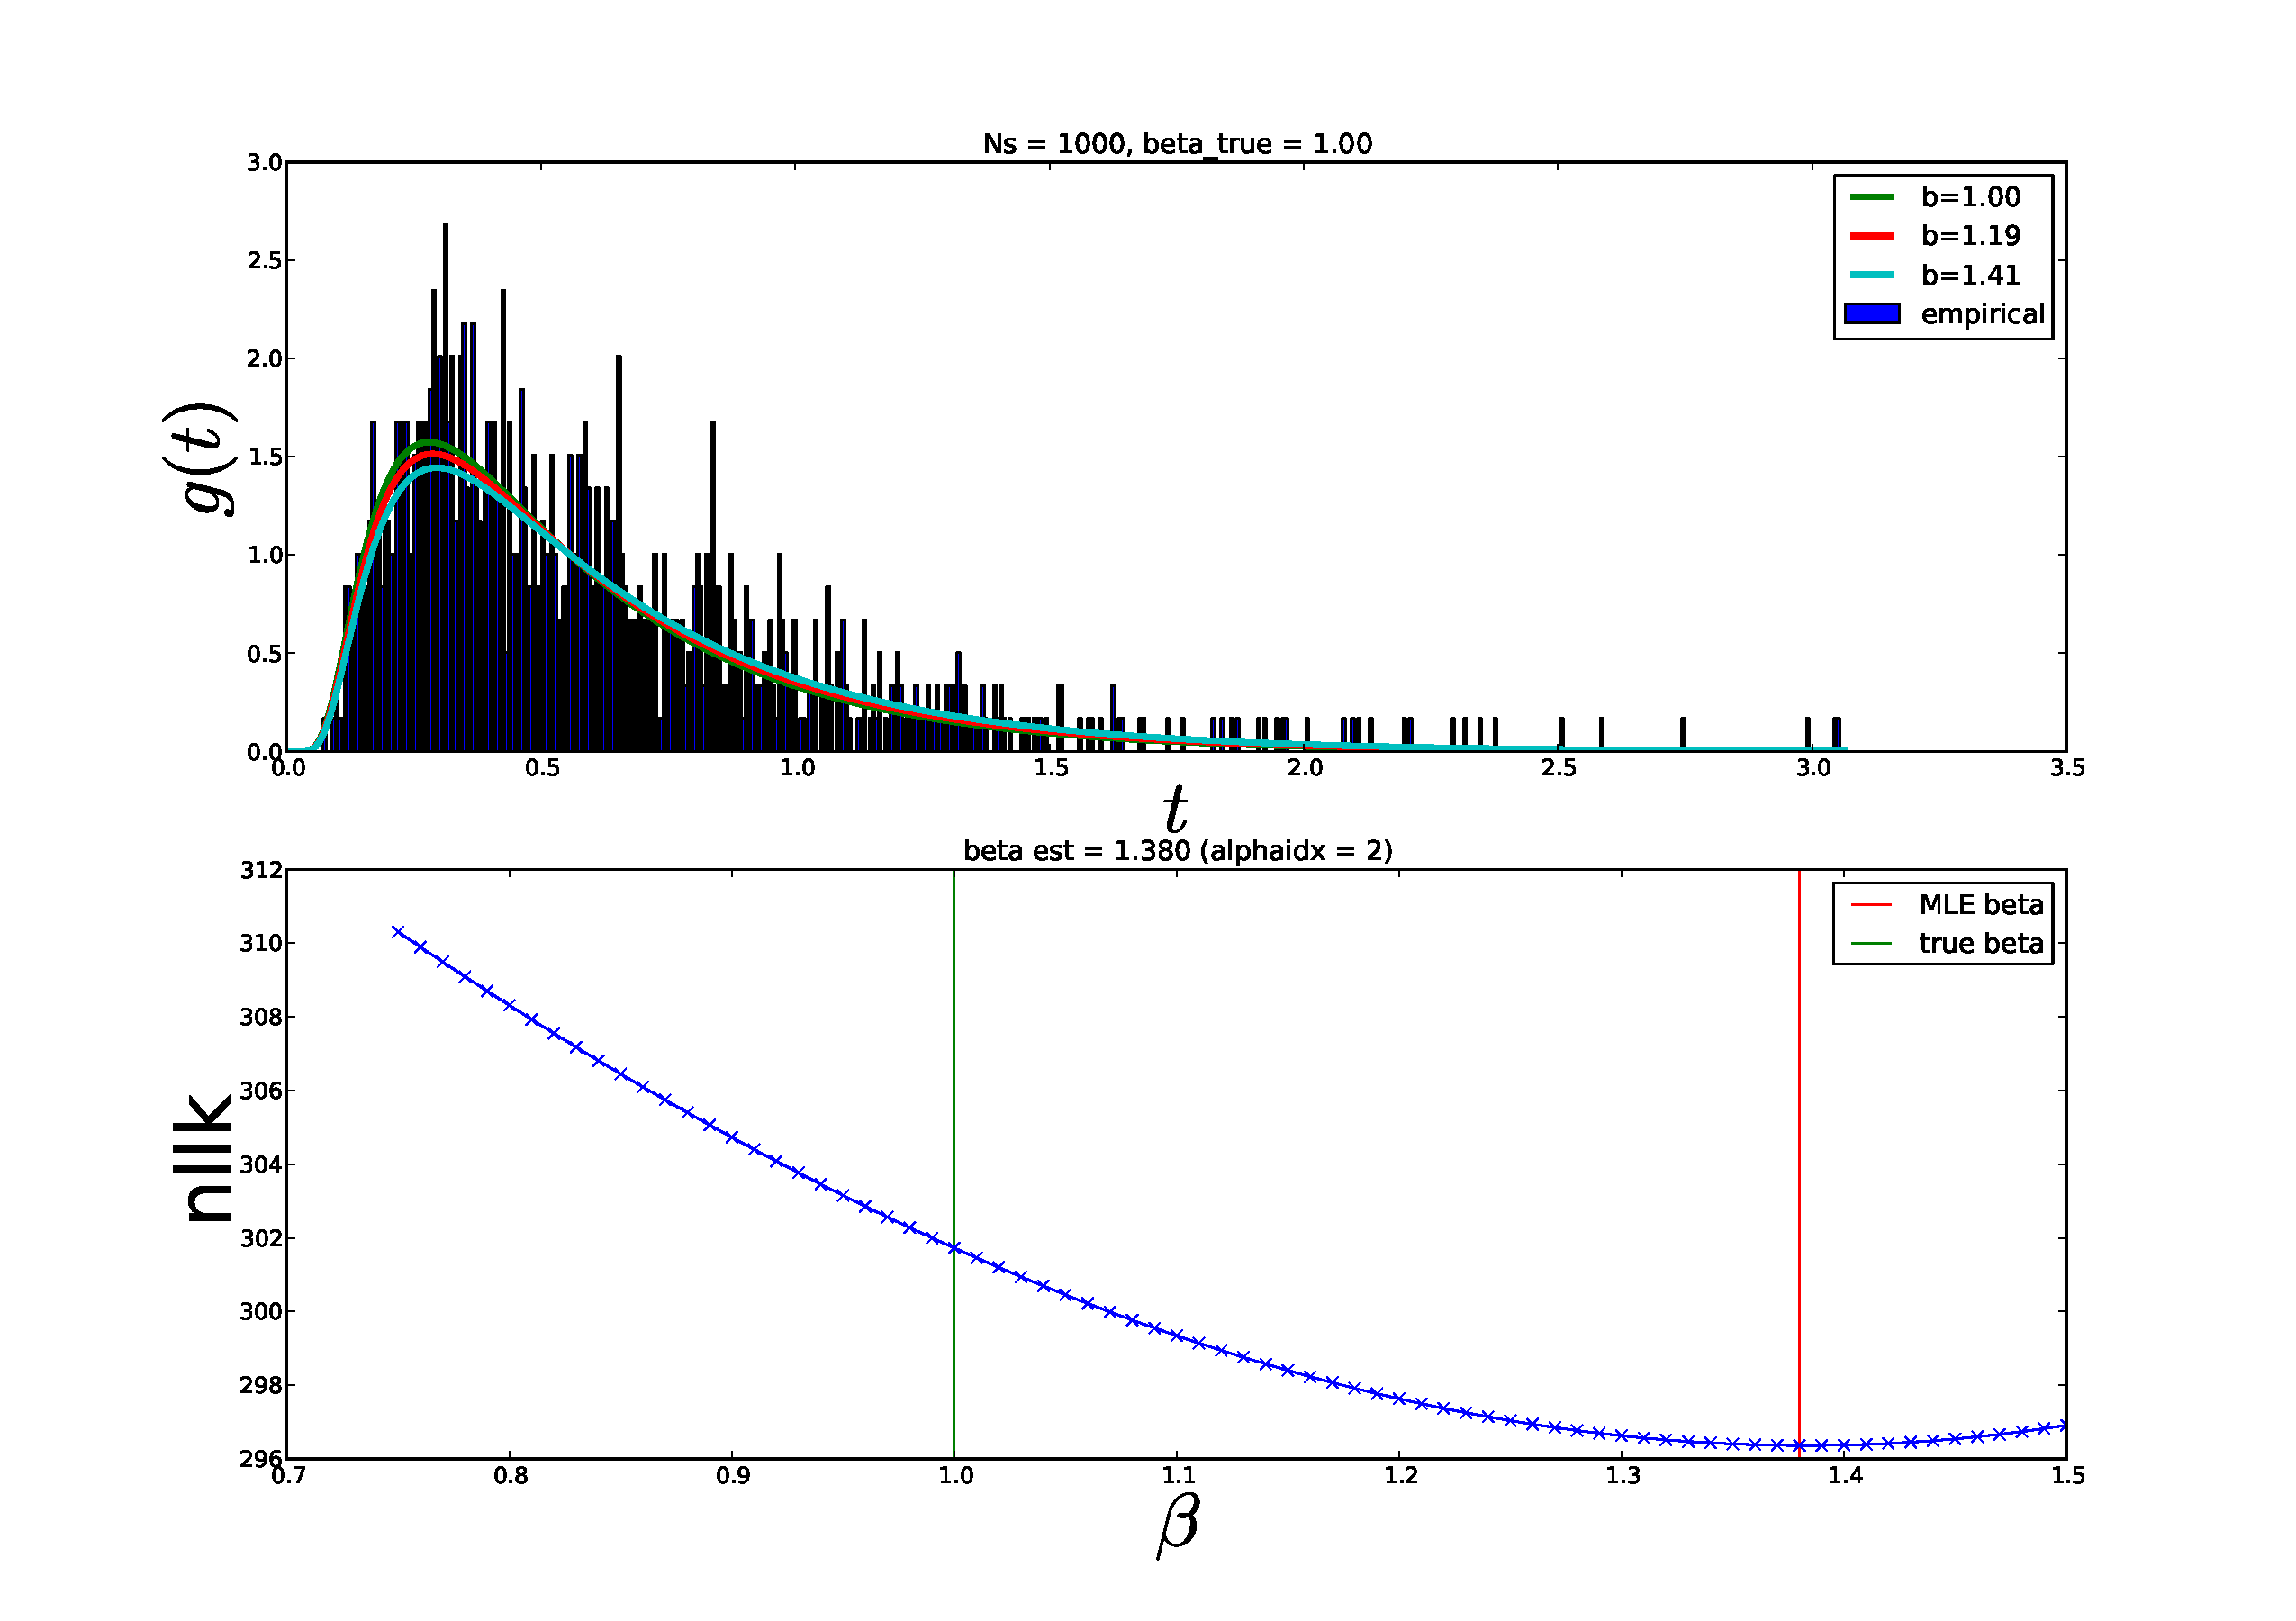
\includegraphics[width=.75\textwidth]
{Figs/HitTime_MI_TauChar_Adjoint_Estimate/Adjoint_TauChar_Estimator_estimatorWorkbench_b=0x1000_a2.pdf}
}
\caption[labelInTOC]{Example of Empirical vs. Analytical Hitting time
distributions and the associated log-likelihoods. $N_s = 1e3$}
\label{fig:log_likelihood_beta_examples_1000}
\end{center}
\end{figure} 


\begin{figure}[h]
\begin{center}
\subfloat[opt]
{
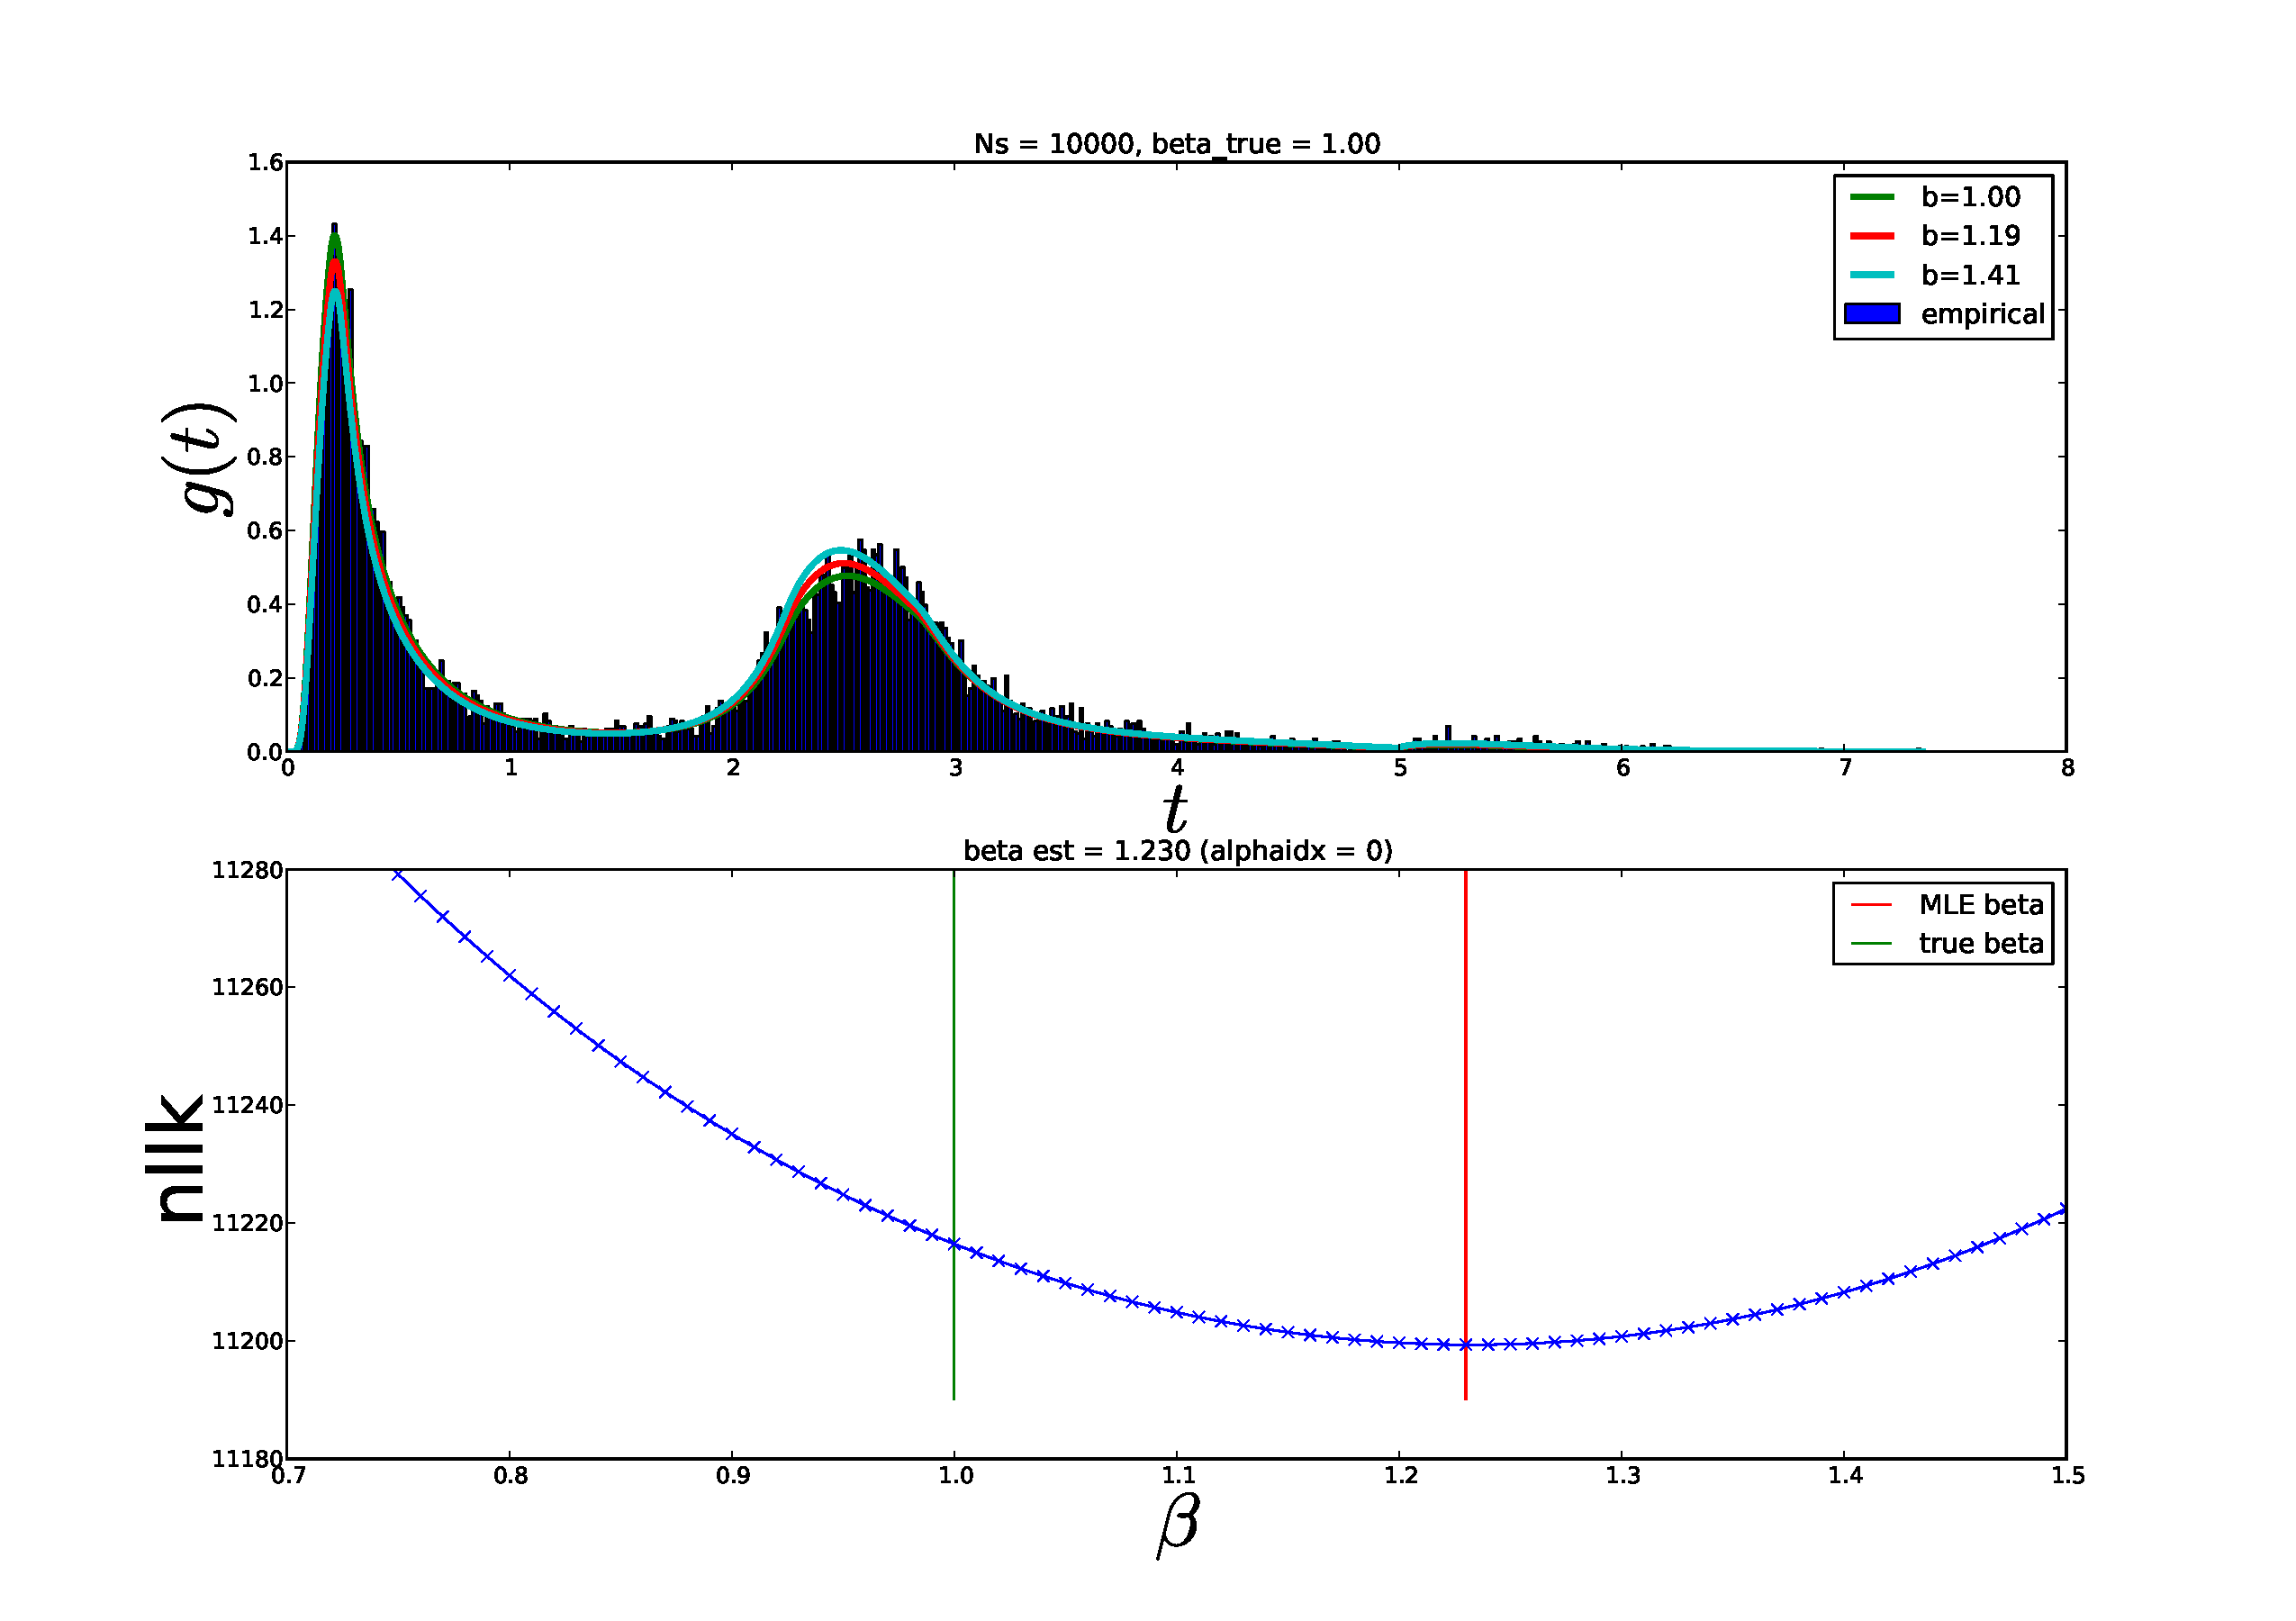
\includegraphics[width=.75\textwidth]
{Figs/HitTime_MI_TauChar_Adjoint_Estimate/Adjoint_TauChar_Estimator_estimatorWorkbench_b=0x10000_a0.pdf}
}
\\
\subfloat[crit]
{
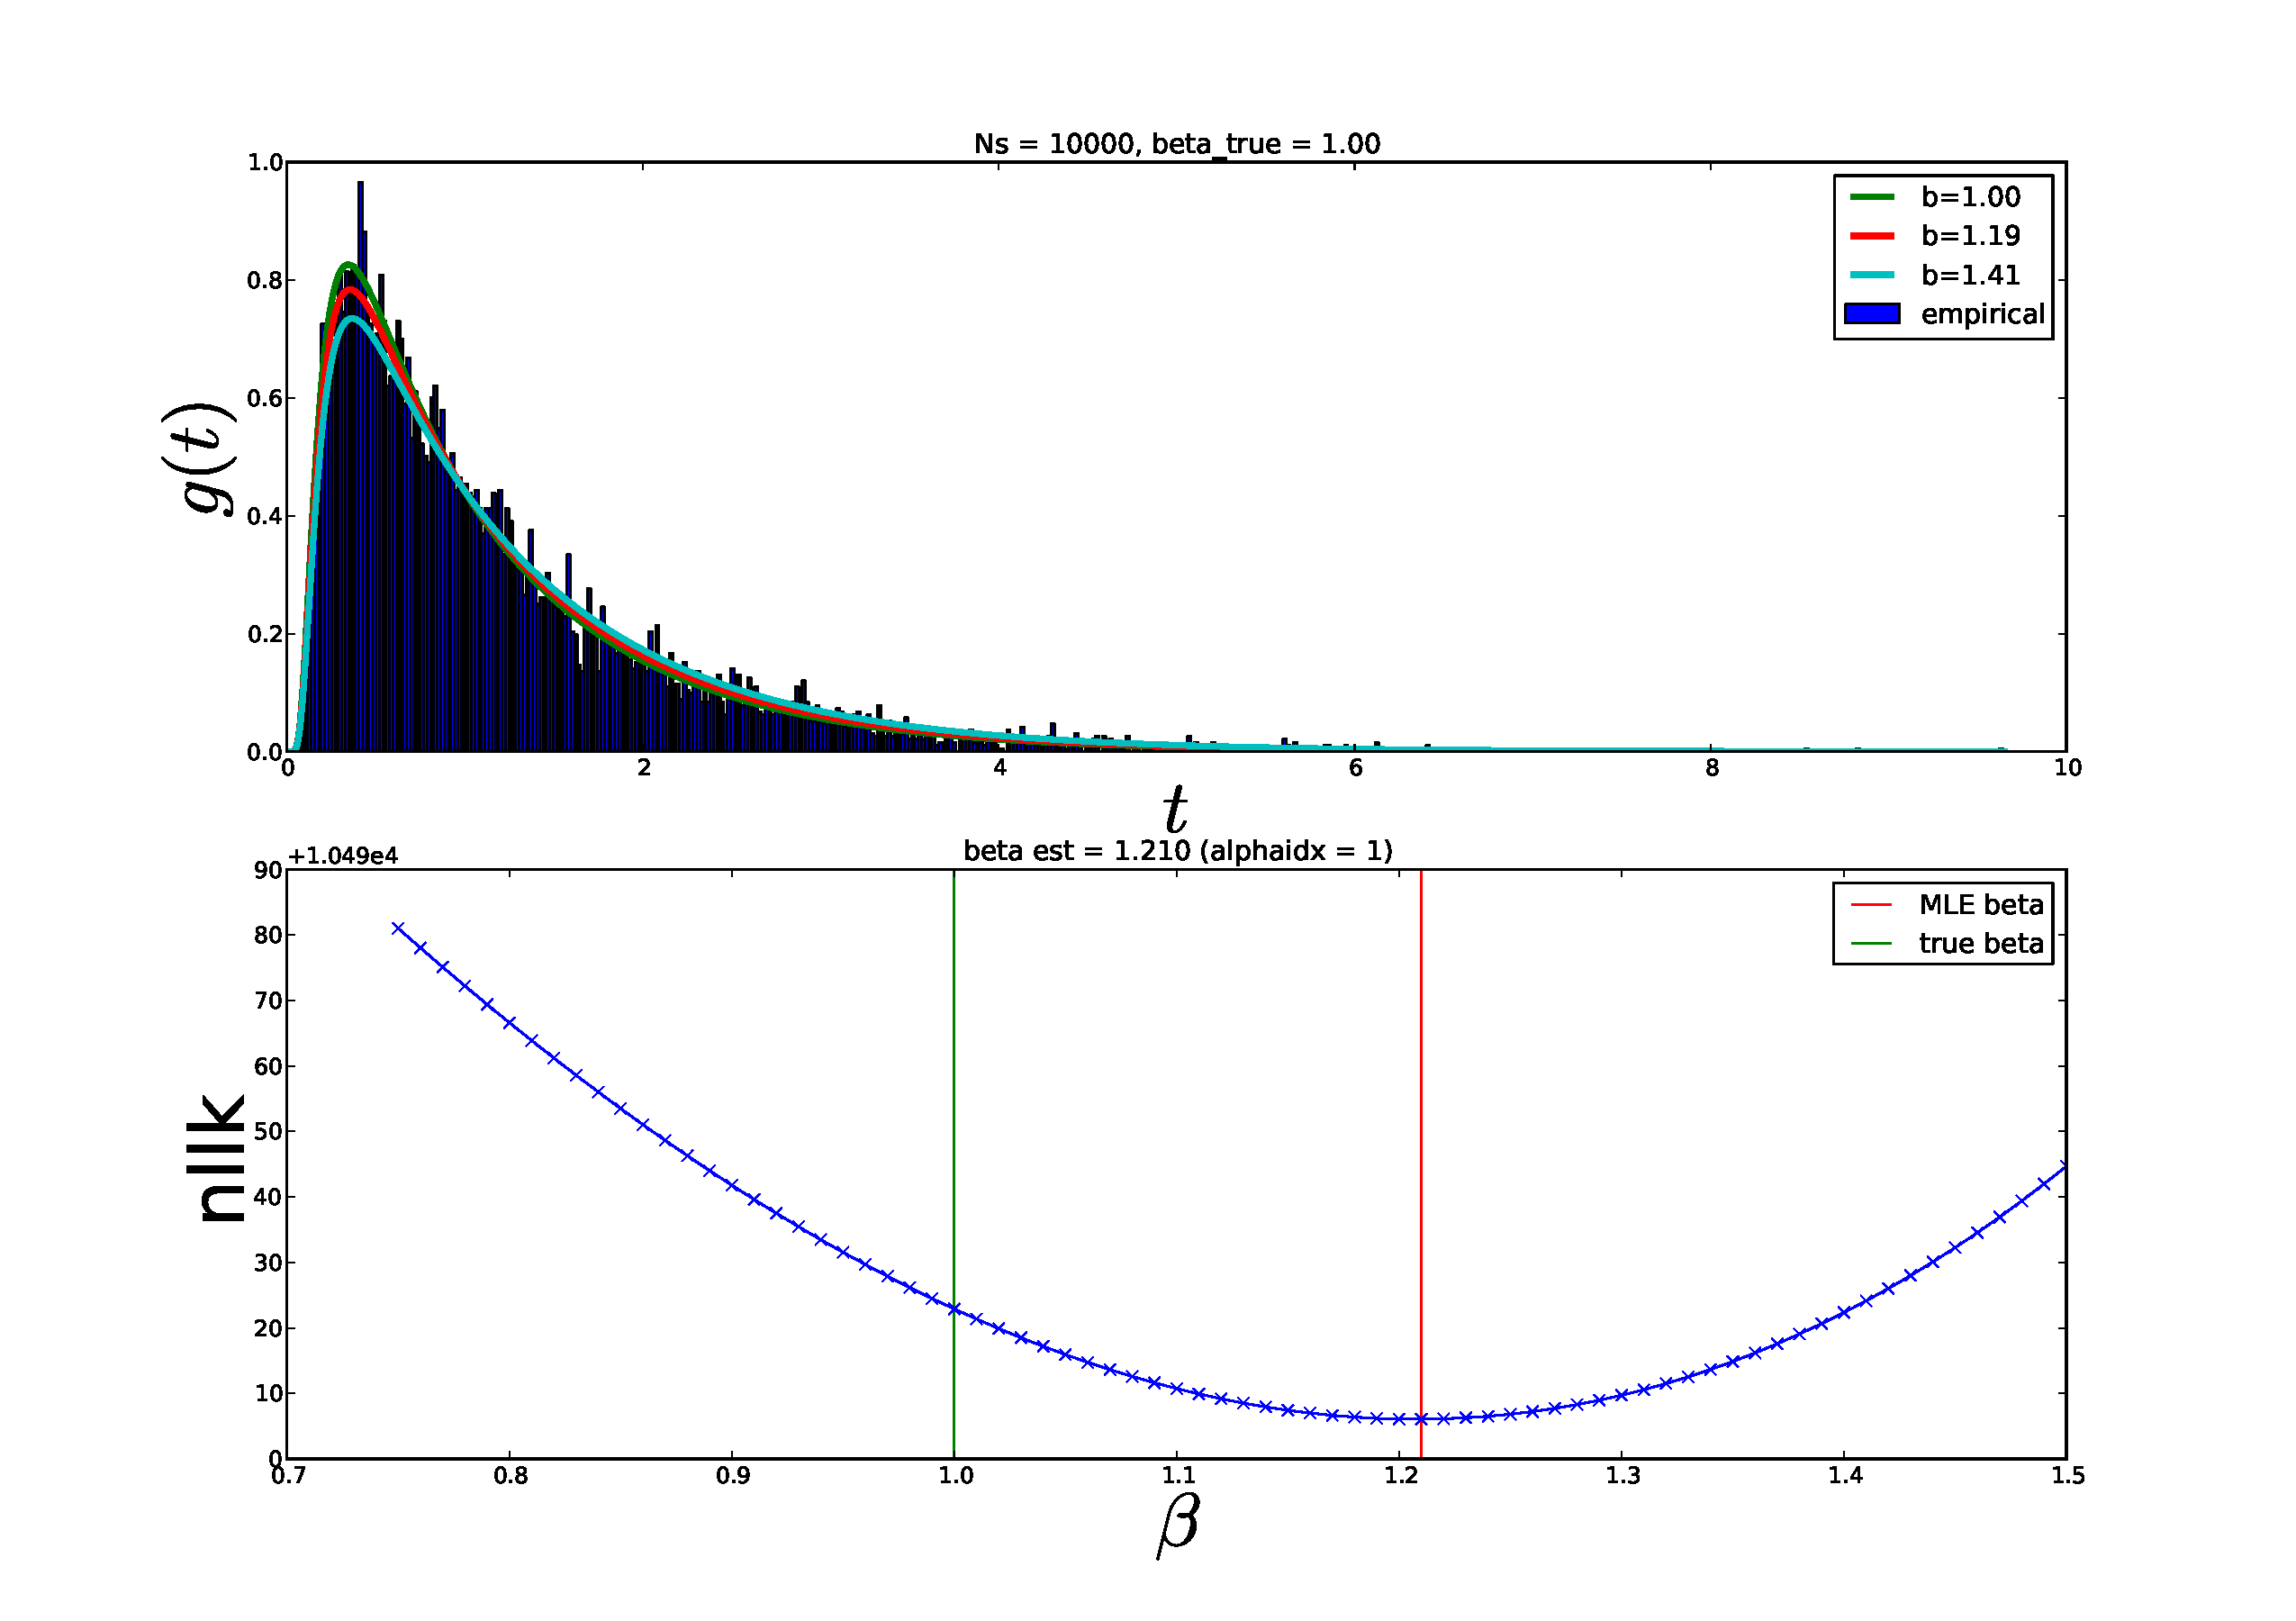
\includegraphics[width=.75\textwidth]
{Figs/HitTime_MI_TauChar_Adjoint_Estimate/Adjoint_TauChar_Estimator_estimatorWorkbench_b=0x10000_a1.pdf}
}
\\ 
\subfloat[max]
{
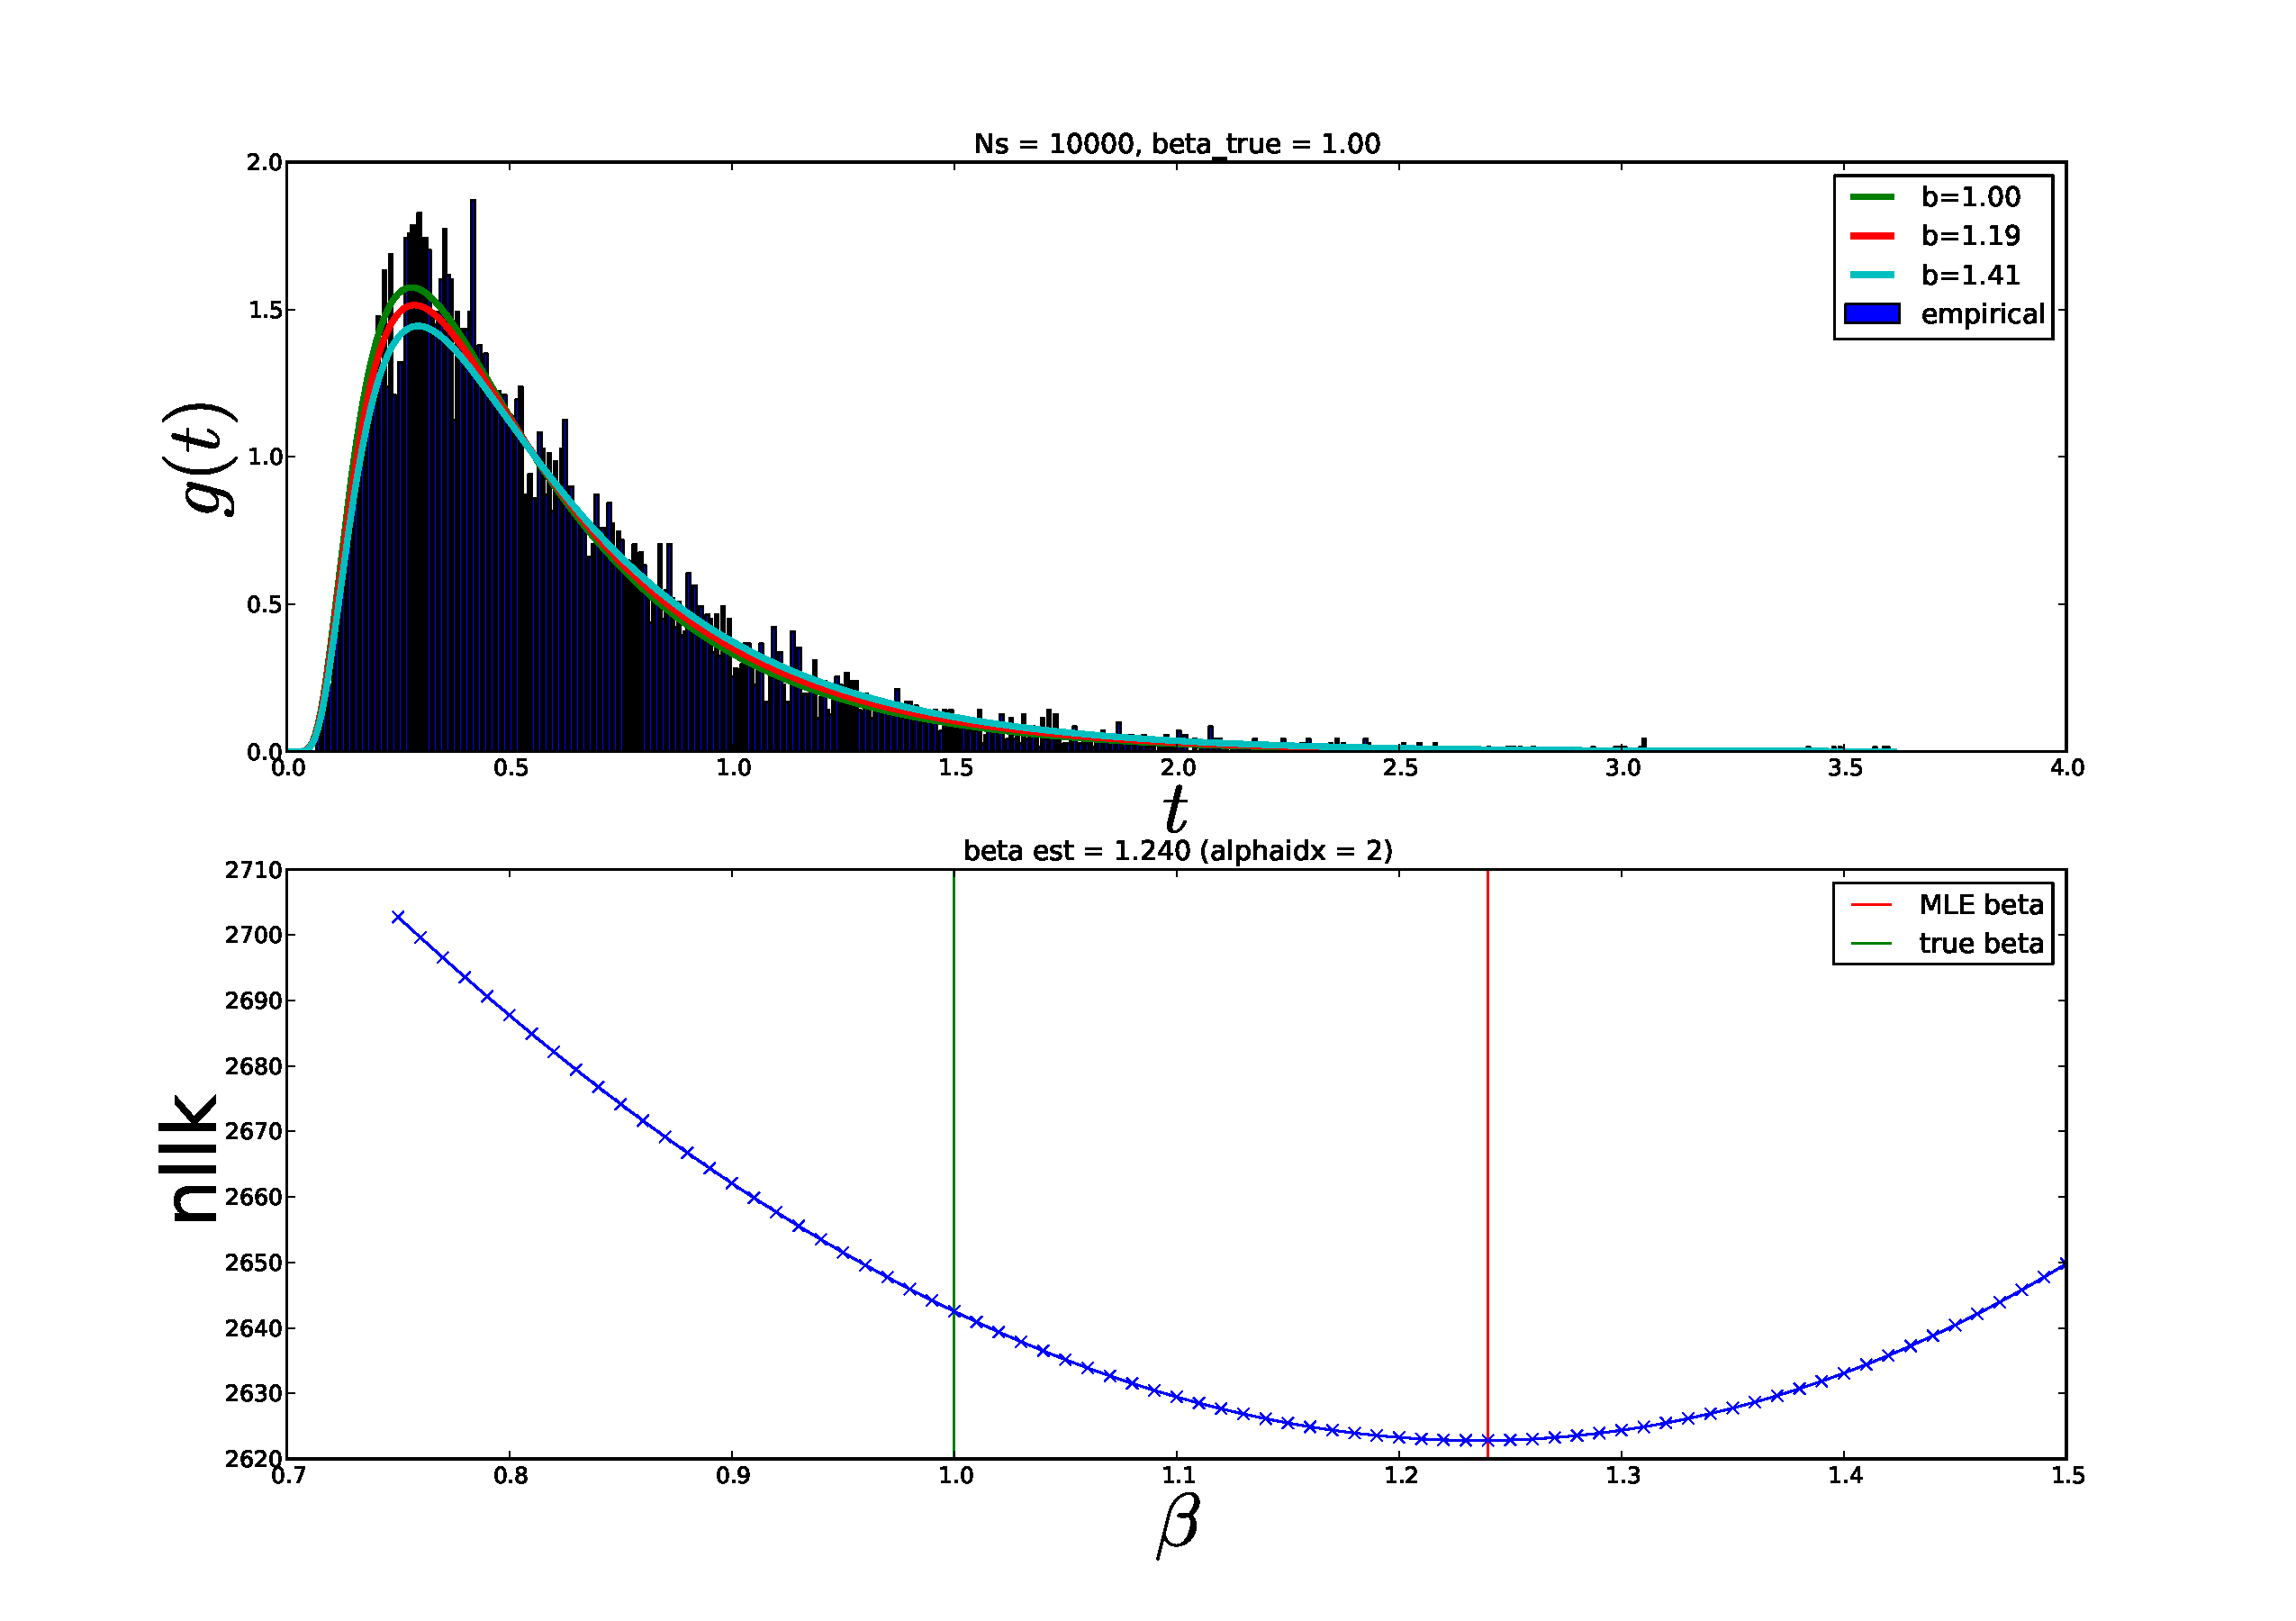
\includegraphics[width=.75\textwidth]
{Figs/HitTime_MI_TauChar_Adjoint_Estimate/Adjoint_TauChar_Estimator_estimatorWorkbench_b=0x10000_a2.pdf}
}
\caption[labelInTOC]{Same as \cref{fig:log_likelihood_beta_examples_1000}, but
with  $N_s = 1e4$. Notice that ( but only slightly ) the 'opt' control tilts in
the right direction for the $\b$ estimate (i.e. towards 1). }
\label{fig:log_likelihood_beta_examples_10000}  
\end{center}
\end{figure}

\begin{figure}[h] 
\begin{center}
\subfloat[opt]
{
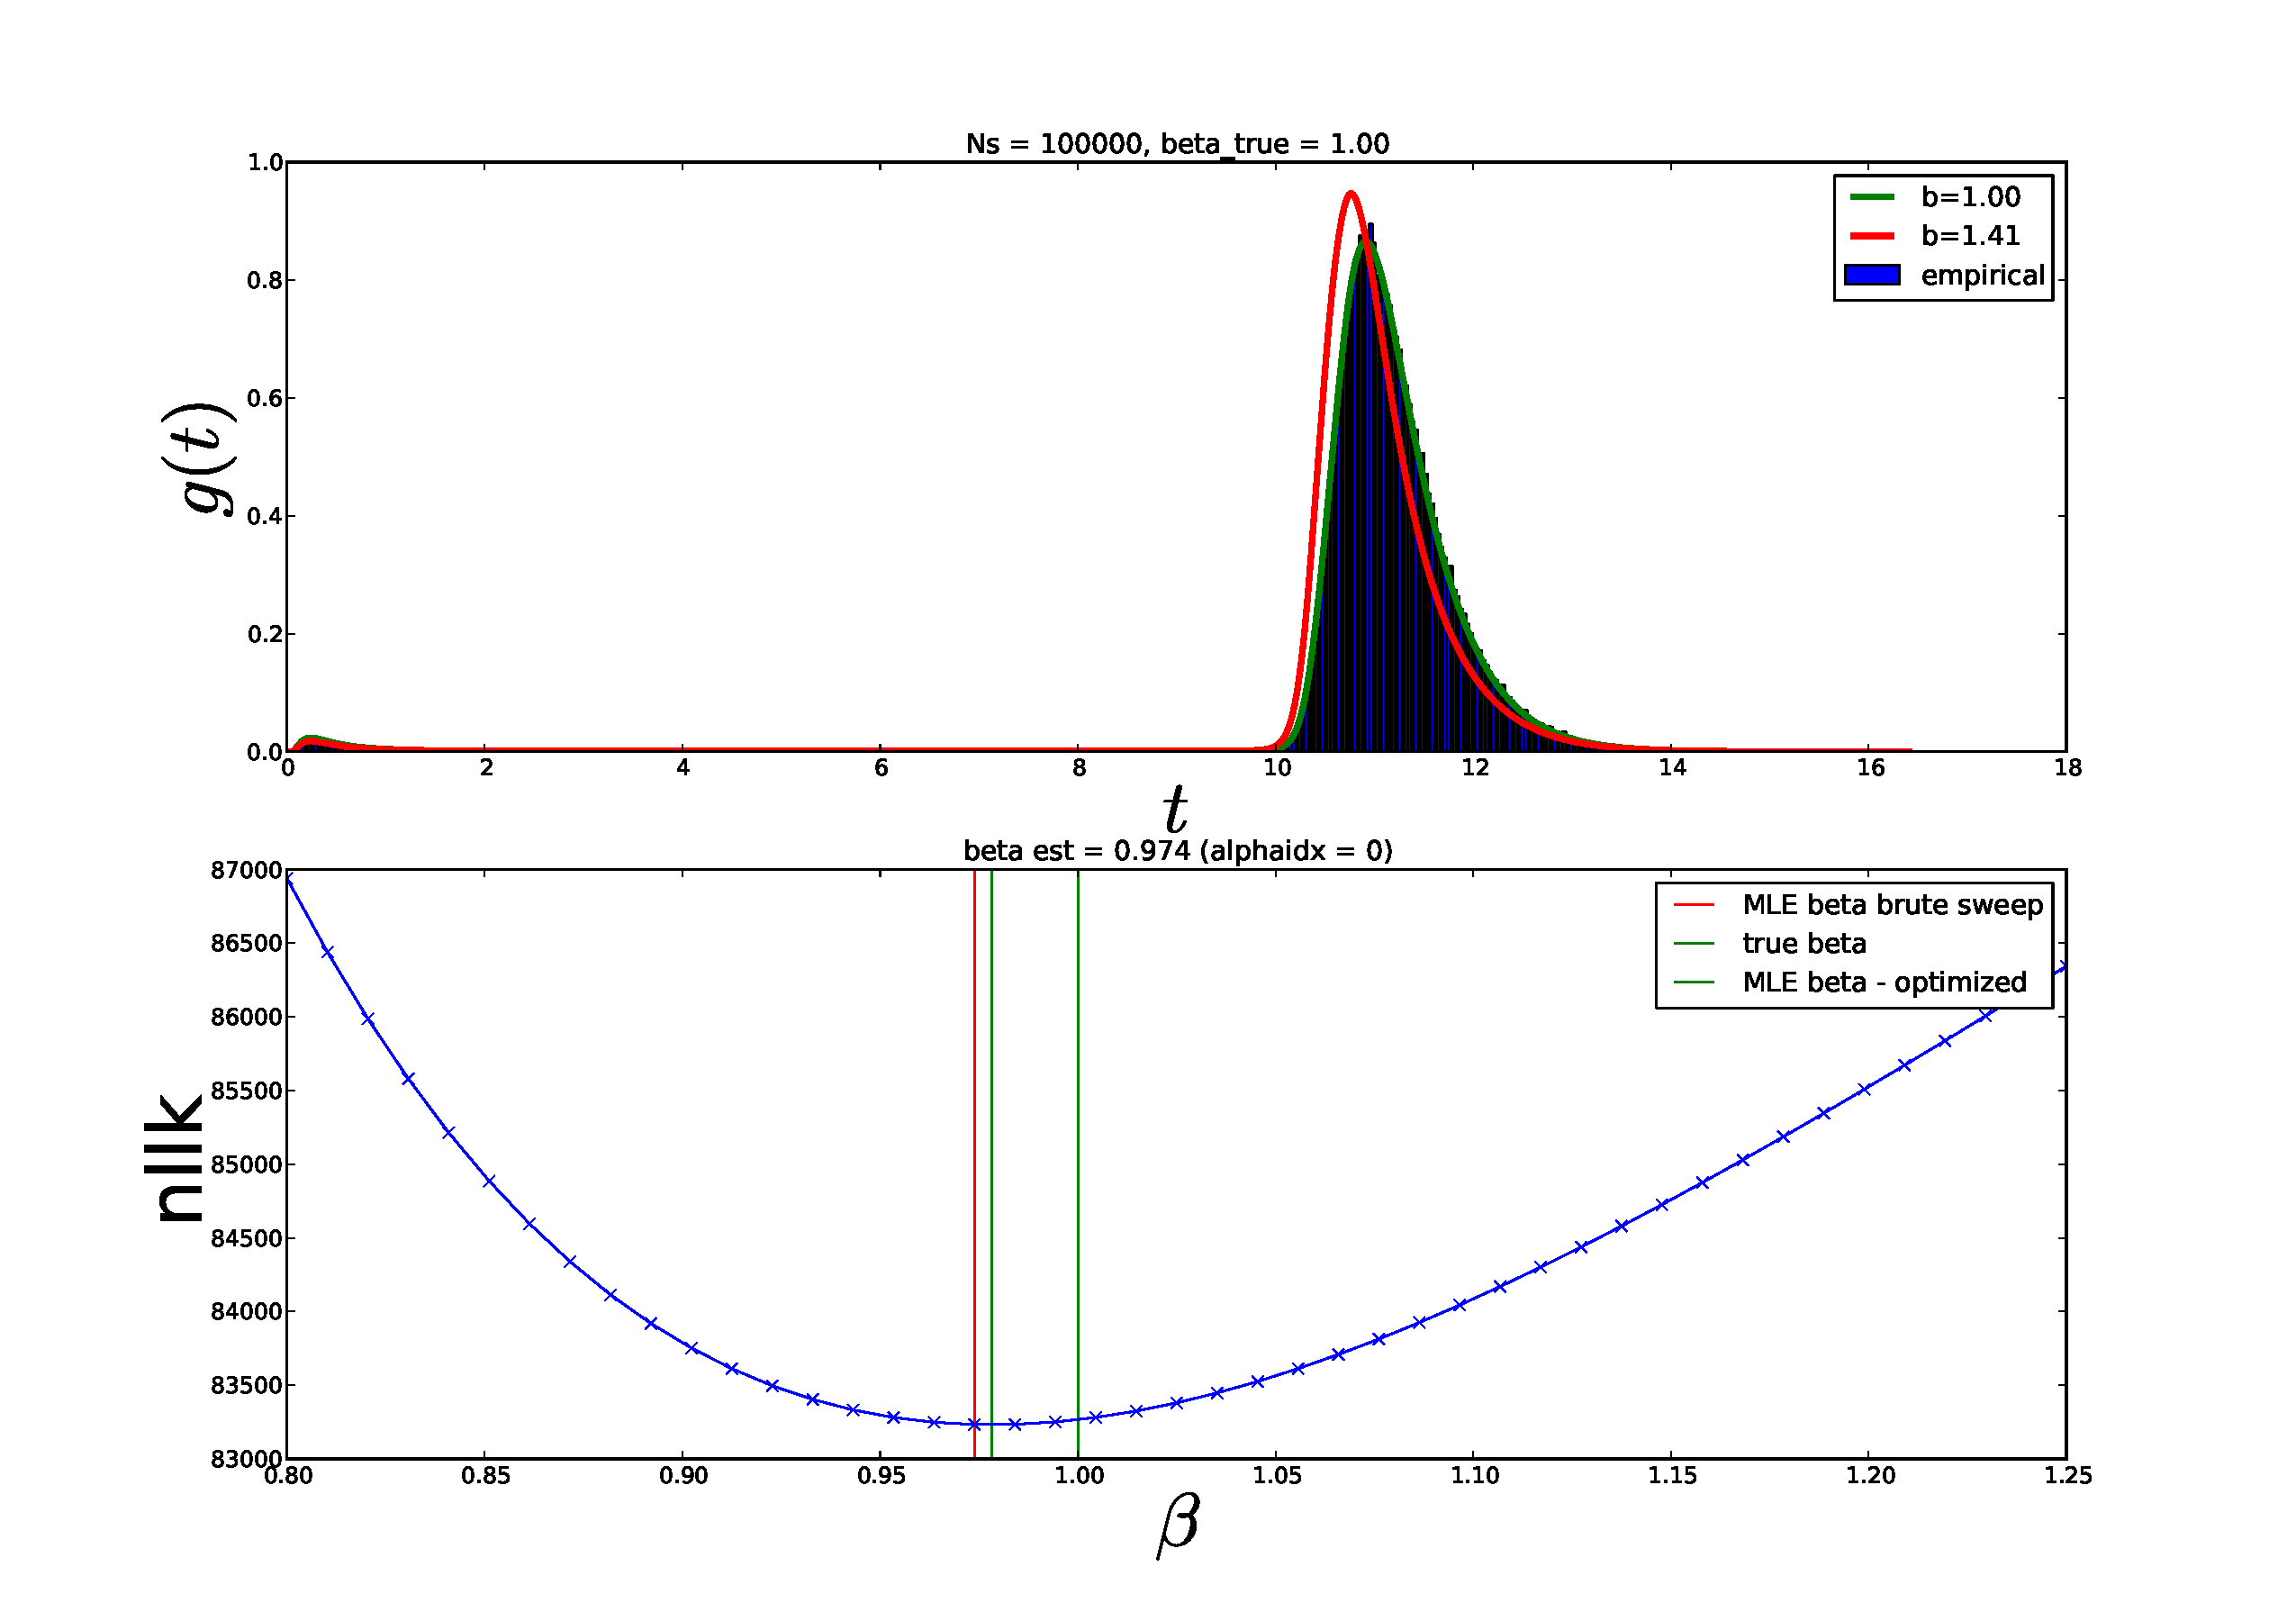
\includegraphics[width=.75\textwidth]
{Figs/HitTime_MI_TauChar_Adjoint_Estimate/Adjoint_TauChar_Estimator_estimatorWorkbench_b=0x100000_a0.pdf}
}
\\
\subfloat[crit]
{
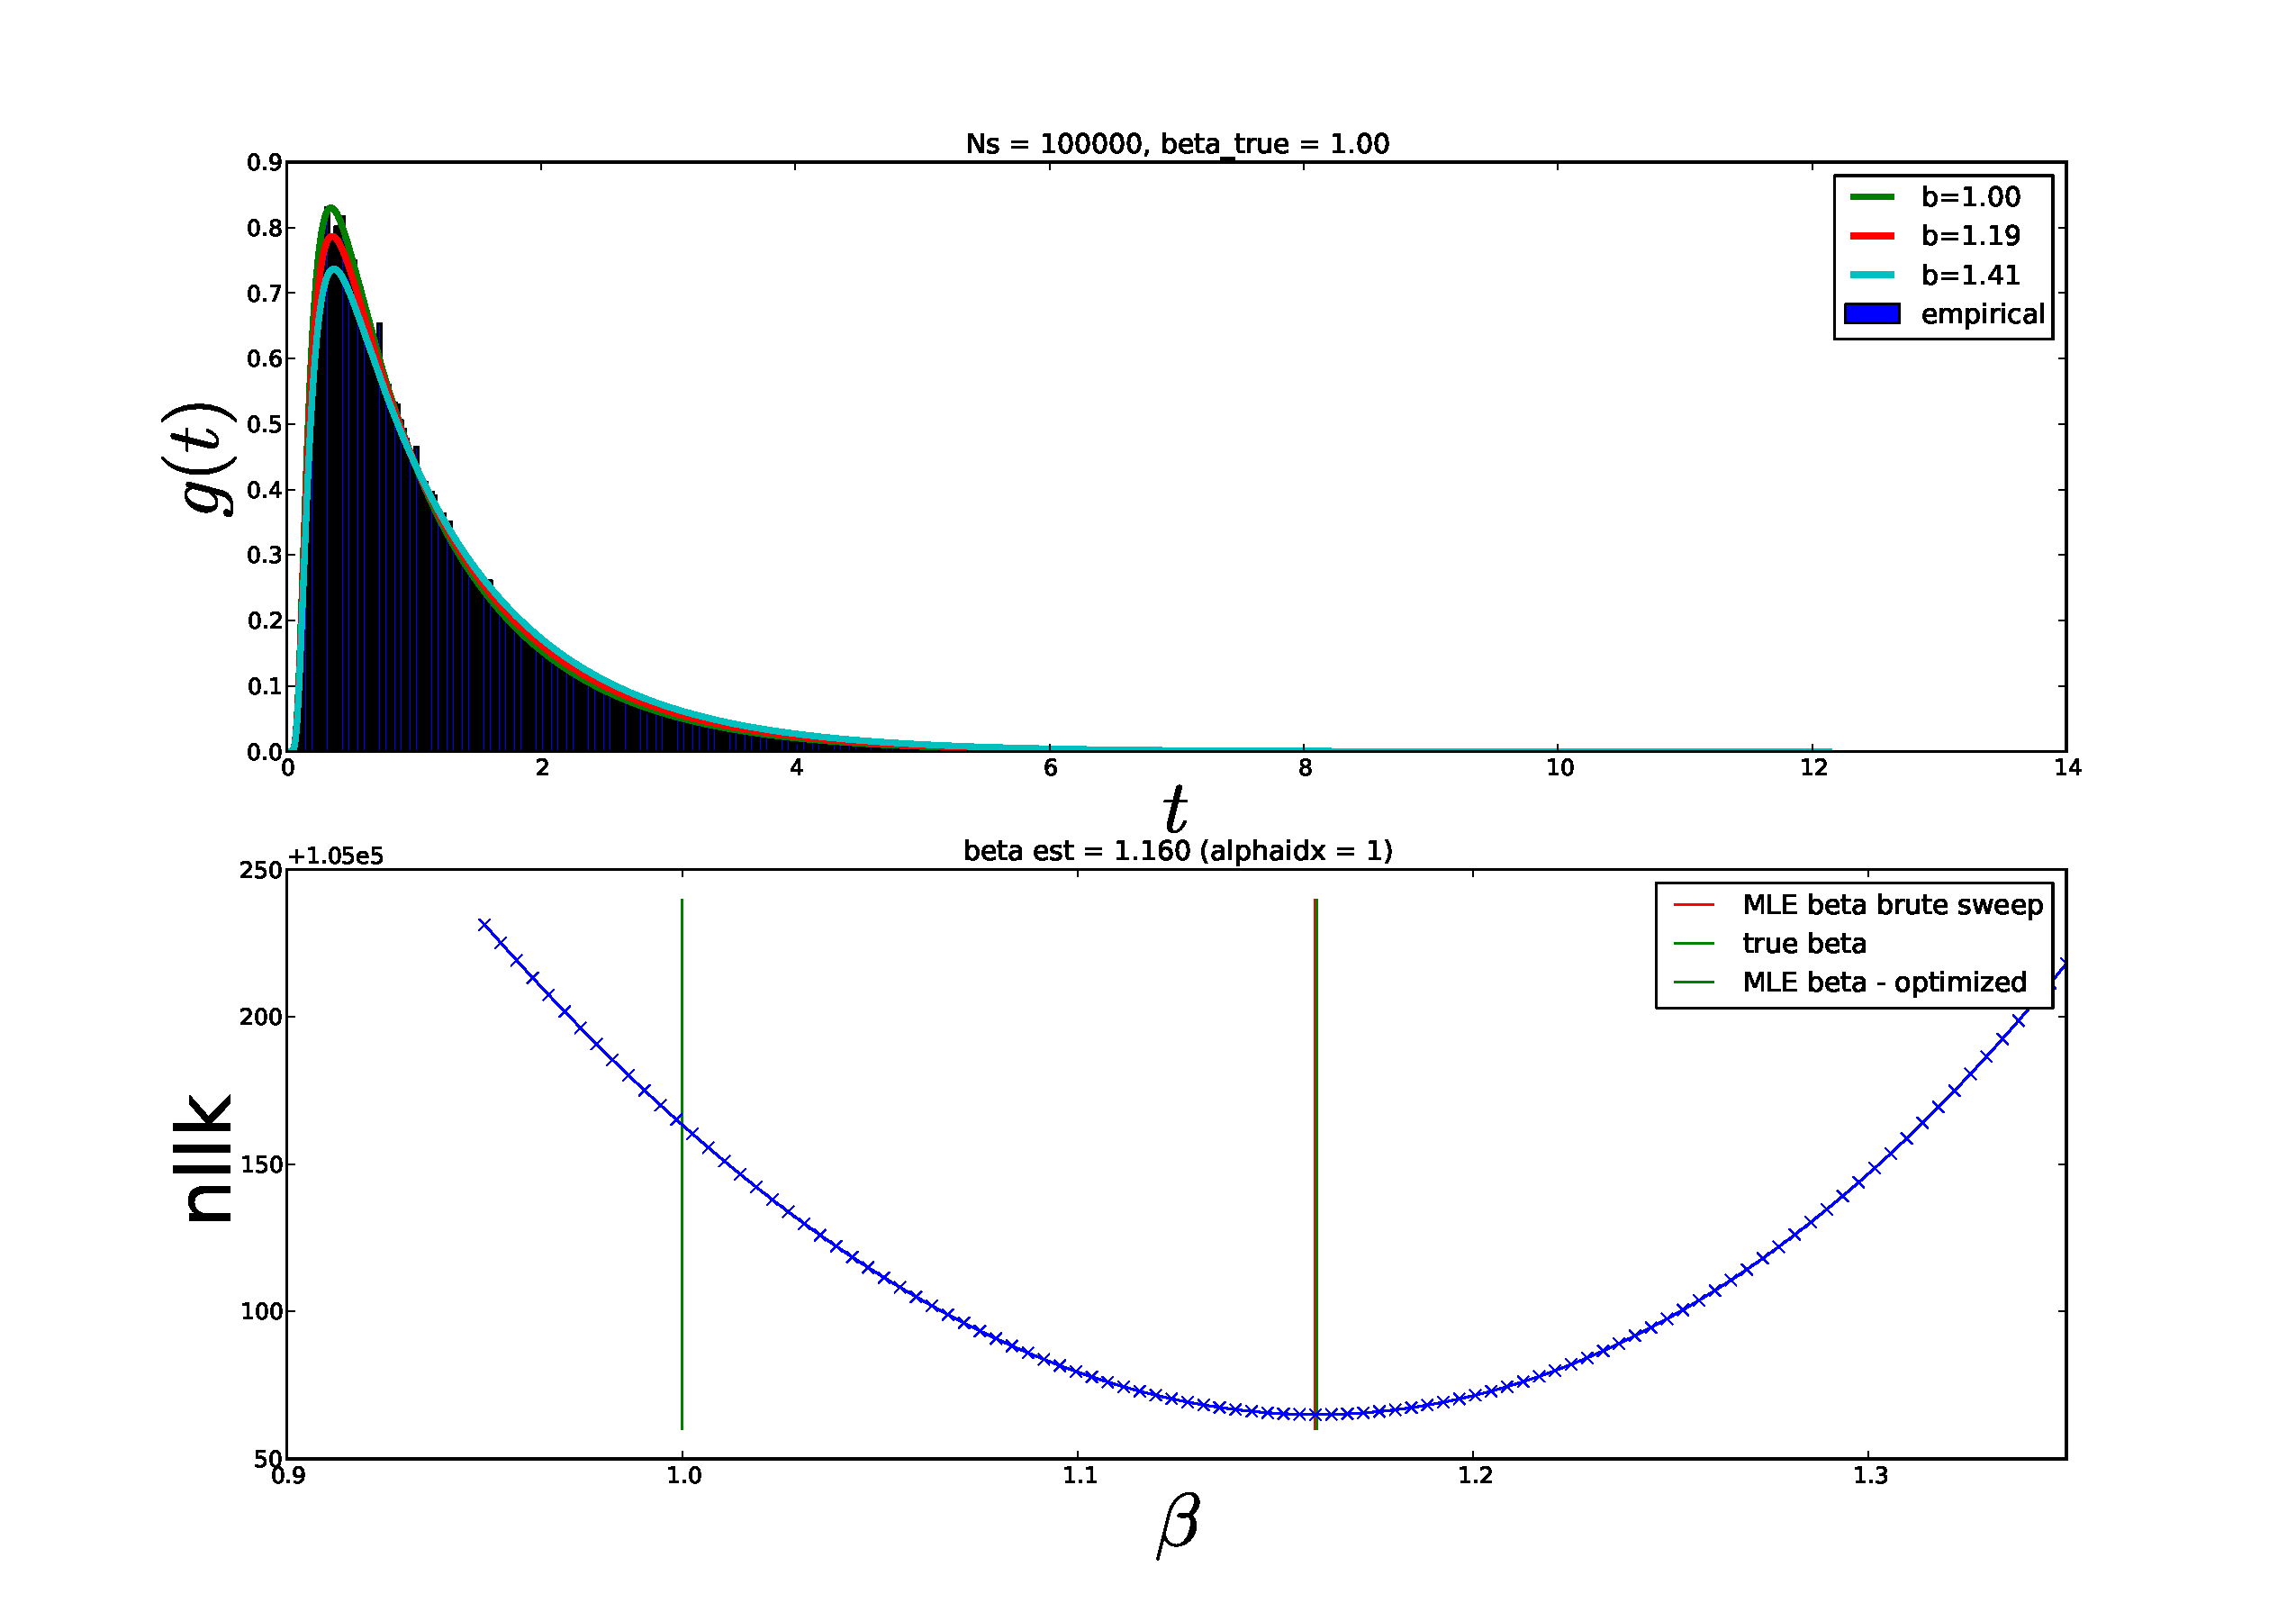
\includegraphics[width=.75\textwidth]
{Figs/HitTime_MI_TauChar_Adjoint_Estimate/Adjoint_TauChar_Estimator_estimatorWorkbench_b=0x100000_a1.pdf}
}
\\
\subfloat[max]
{
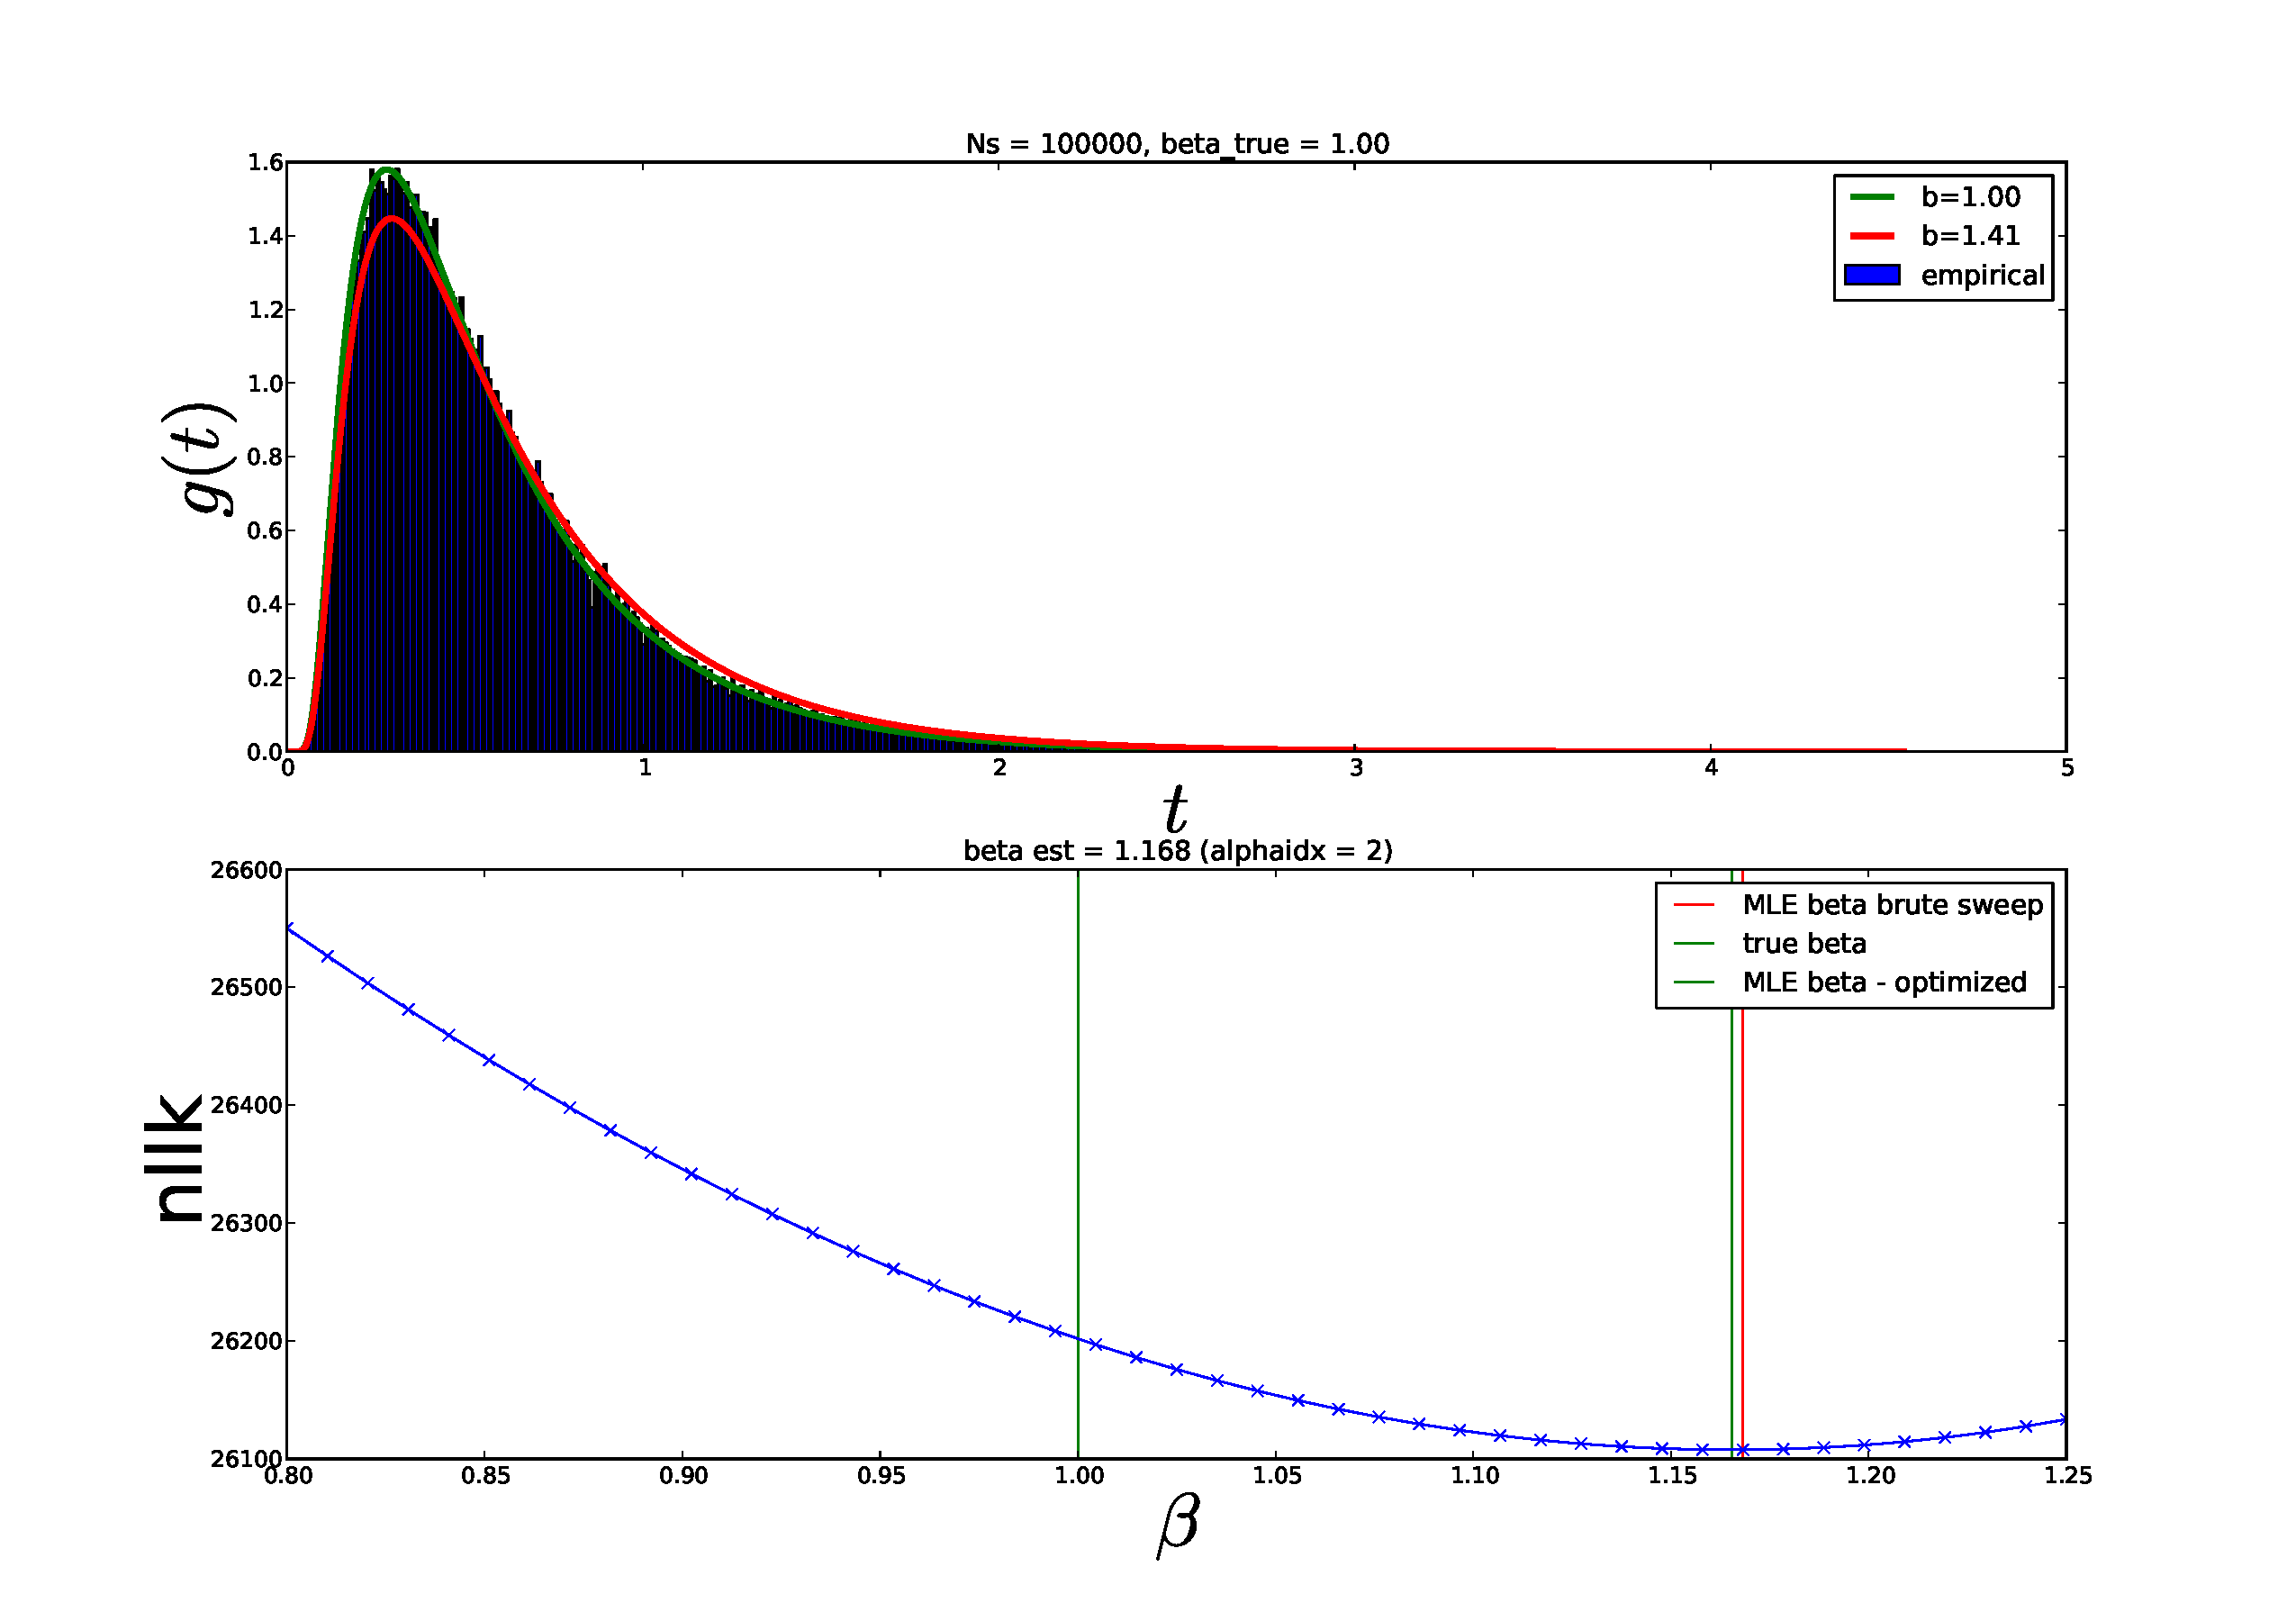
\includegraphics[width=.75\textwidth]
{Figs/HitTime_MI_TauChar_Adjoint_Estimate/Adjoint_TauChar_Estimator_estimatorWorkbench_b=0x100000_a2.pdf}
}
\caption[labelInTOC]{Same as  
\cref{fig:log_likelihood_beta_examples_1000,fig:log_likelihood_beta_examples_10000}
but with $N_s = 1e5$ hits}
\label{fig:log_likelihood_beta_examples_100000}
\end{center}
\end{figure}  
 -
\clearpage

\subsubsection{Batch Performance of the perturbations over the estimators.}
As is we have 3 candidates for perturbing the hitting times: 
\begin{enumerate}
  \item 
the optimal gradient-ascent-based  control $\a_{opt}$ (see
\cref{fig:hitting_time_density_g_aopt_bprior} top panel)
\item   the 'critical' constant control
$\a_{crit}$, ($\a_{crit}(t) = 1/\b$)
\item  the max constant control, $\amax$ ($=2$)
\end{enumerate} 

We now simulate $N_b = 100$ blocks of $N_s=1000$ hitting times each for the
3 alphas and then estimate $\b$ over each set using MaxLikelihood over our
computed expression for the density, $g(t|\tc; \a(t) )$). Examples for
differnt $N_s$ of the hitting time empirical
distribution are shown in \cref{fig:log_likelihood_beta_examples_1000} etc..
Naturally, for each control, we use the same gaussian random draws per block of $N_s$ Hitting of times).
%\usepackage{graphics} is needed for \includegraphics
% \begin{figure}[htp]
% \begin{center}
%   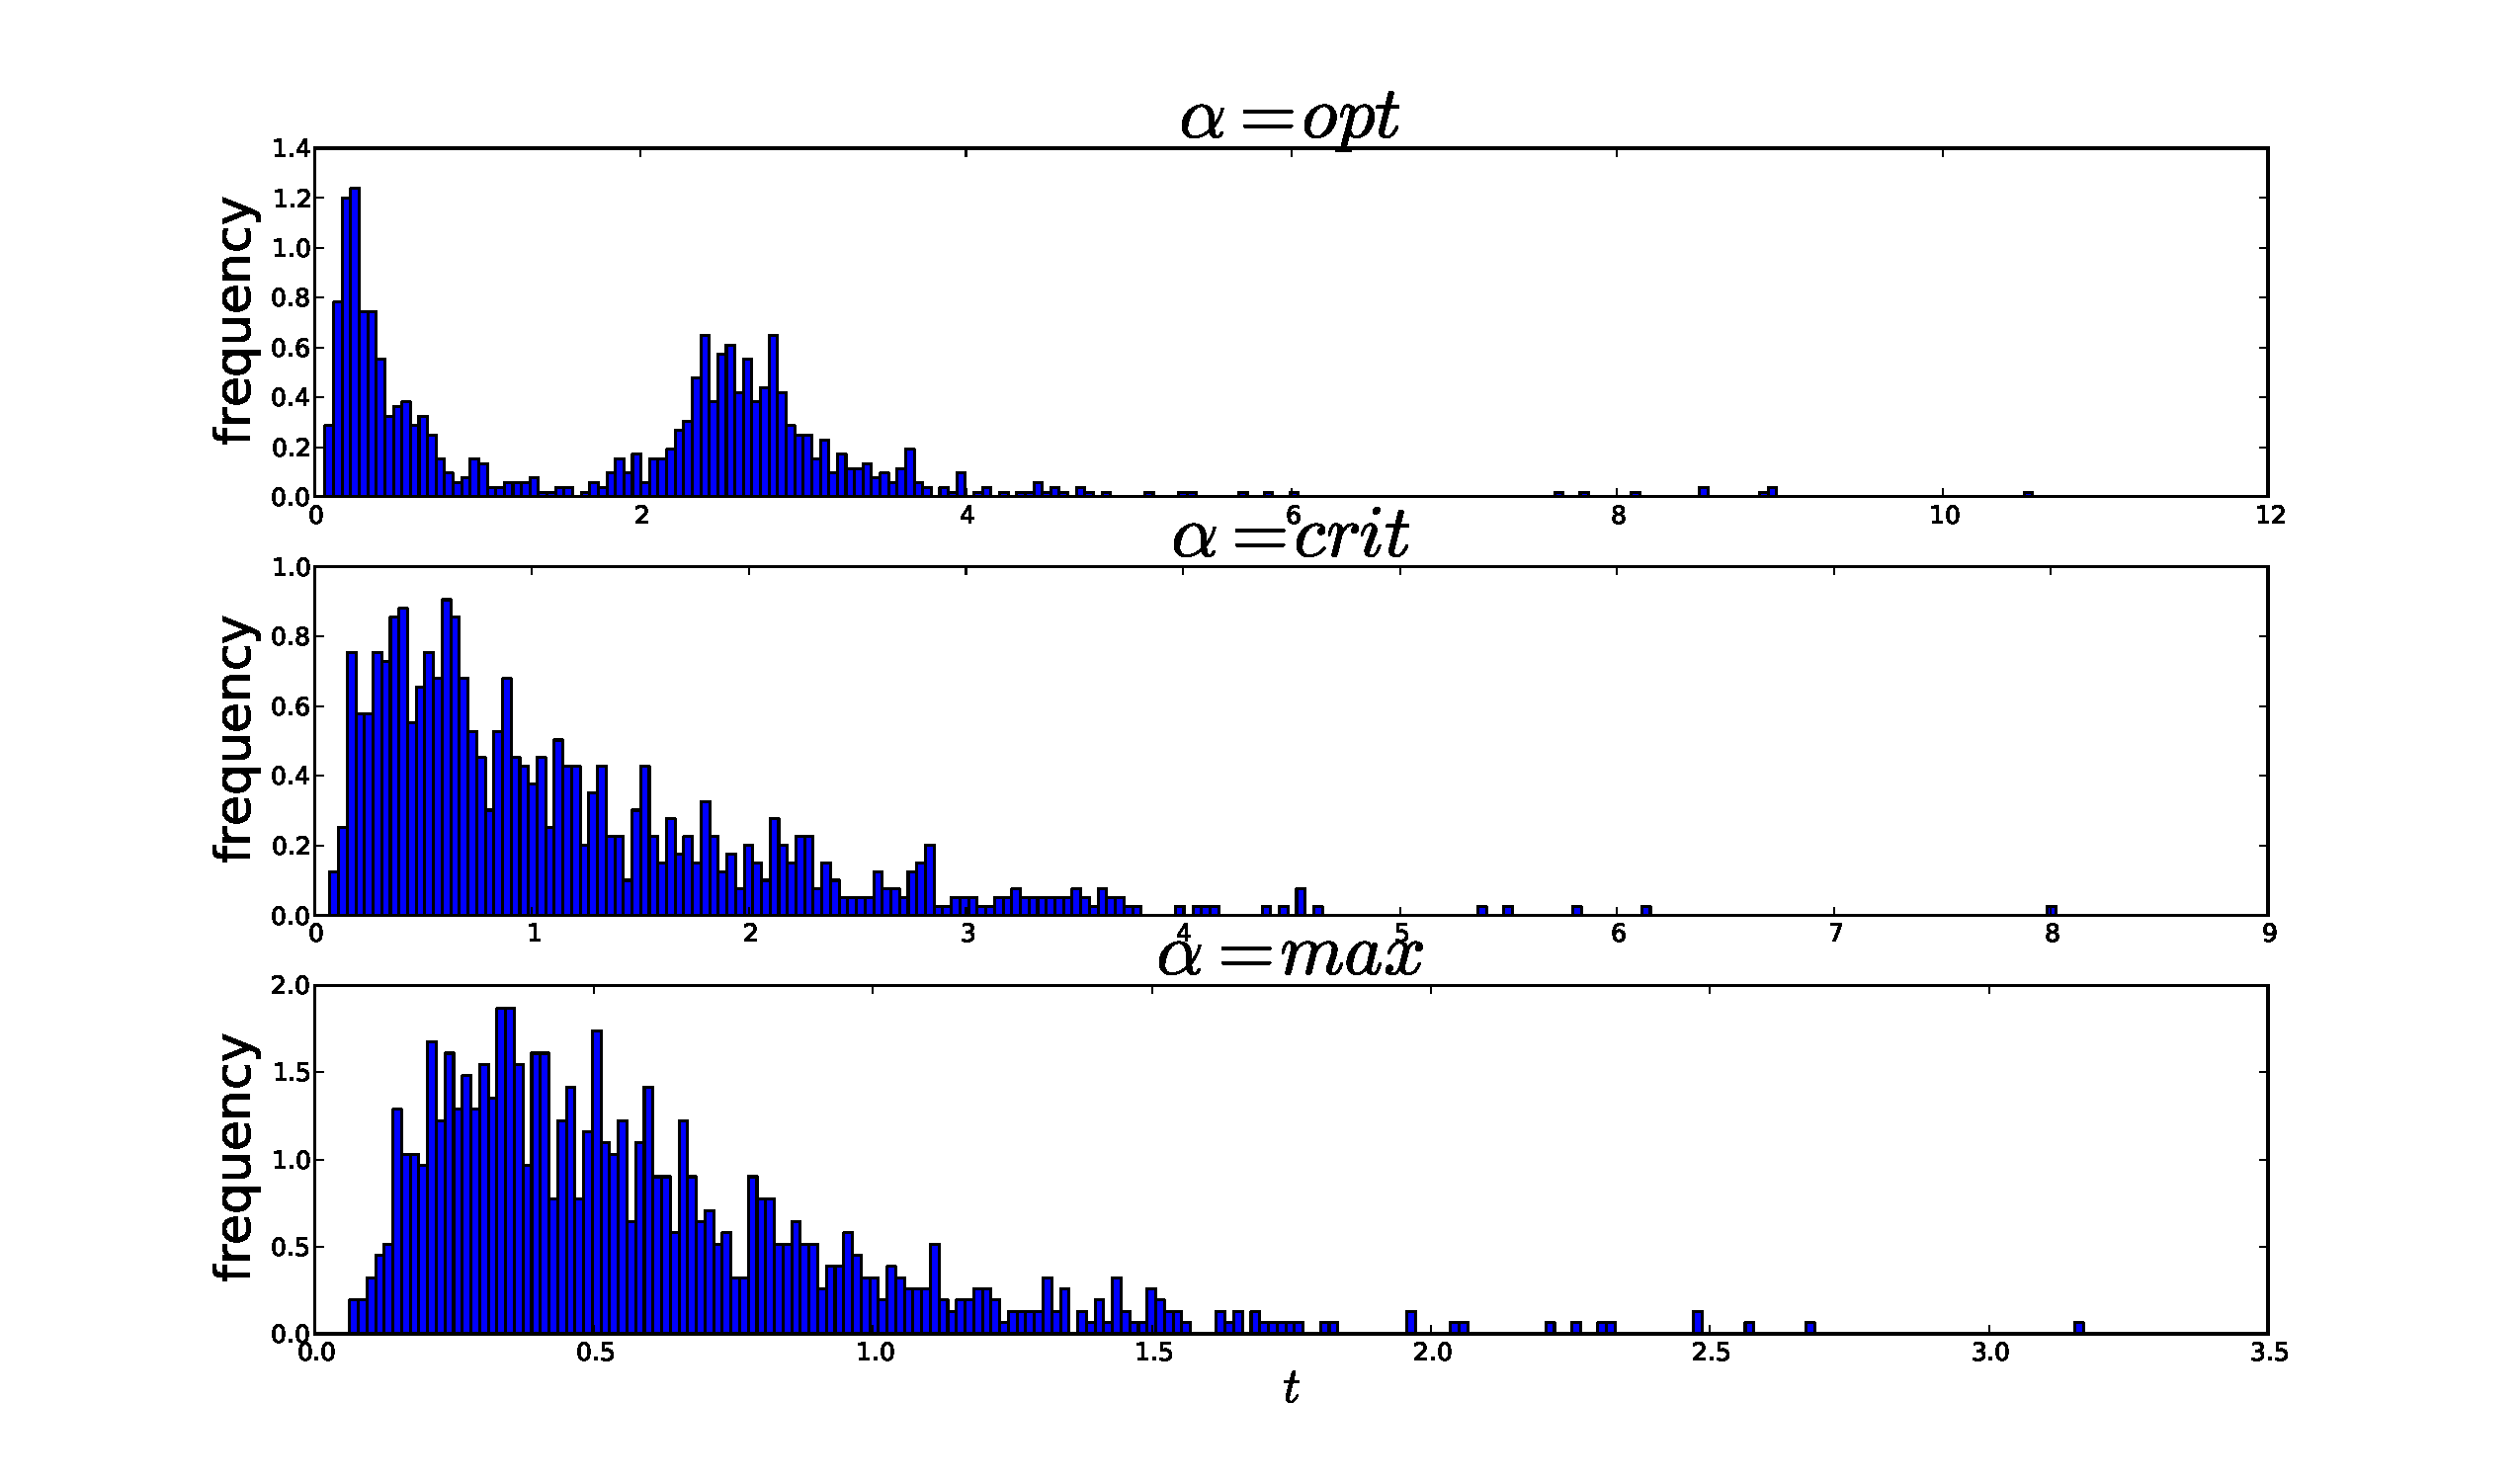
\includegraphics[width=\textwidth]{Figs/HitTime_MI_TauChar_Adjoint_Estimate/three_pt_prior_thits_distn.pdf}
%   \caption[labelInTOC]{Empirical Hitting-TIme distributions for the different
%   choices of $\a$}
%   \label{fig:empirical_hitting_times_3alphas}
% \end{center}
% \end{figure}

The estimation results are tabulated in in
\cref{tab:beta_estimates_from_hitting_times_different_alphas}.

\begin{table}
\subfloat[$N_b=1000, N_s = 1e2$]{
\begin{tabular}{ccc}
\input{../OptEstimate/Figs/HitTime_MI_TauChar_Adjoint_Estimate/beta_hit_time_100.txt}
\end{tabular}
}
\subfloat[$N_b=100, N_s = 1e3$]{
\begin{tabular}{ccc}
\input{../OptEstimate/Figs/HitTime_MI_TauChar_Adjoint_Estimate/beta_hit_time_1000.txt}
\end{tabular}
}\\
\subfloat[$N_b=10, N_s = 1e4$]{
\begin{tabular}{ccc}
\input{../OptEstimate/Figs/HitTime_MI_TauChar_Adjoint_Estimate/beta_hit_time_10000.txt}
\end{tabular}
} 
\subfloat[$N_b=1, N_s = 1e5$]{
\begin{tabular}{ccc}
\input{../OptEstimate/Figs/HitTime_MI_TauChar_Adjoint_Estimate/beta_hit_time_100000.txt}
\end{tabular}
}
\caption{Results for the estimates arising from simulations using various values
of $\a$ (opt, crit, max). In each sub-table there are $N_b$
parameter estimates for each distinct $\a$, with $N_s$ hitting times used to form an $\b-$estimate.
The 'true' value of $\b$ is $\b=1$. }
\label{tab:beta_estimates_from_hitting_times_different_alphas}
\end{table}     
% \begin{table} 
% \caption{$N_b=10$, $N_s = 1e4$  }
% \label{tab:beta_estimates_from_hitting_times_different_alphas_Nhits10000}
% \end{table}   
% \begin{table}
% \begin{tabular}{ccc}
% \input{../OptEstimate/Figs/HitTime_MI_TauChar_Adjoint_Estimate/beta_hit_time_100000.txt}
% \end{tabular}   
% \caption{$N_b=1$, $N_s = 1e5$ (estimator variance is irrelevant here as there is only 1 estimate per alpha)}
% \label{tab:beta_estimates_from_hitting_times_different_alphas_Nhits100000}
% \end{table}  

Comments: It looks like there is a marginal advantage to using the 
Optimal Control, $\a_{opt}$ over the simpler, constant controls. In particular
the bias of the estimates seems to be reduced. The variance of the estimates
seems to be independent of the perturbation\ldots 
 
\clearpage


\section{Online MI Optimization}
Hеre we outline a tentative approach to {\sl online} optimization of the MI,
which means

\begin{enumerate}
  \item Find $\aopt$ using the gradient ascent, for the prior $\rho$
  \item Apply $\aopt$ and measure several $1,2\ldots,N_{s,1}$ hitting times
  $t_k$
  \item Update the $\rho$ into a posterior conditional on the observed $\{t_k\}$
  \item Recalibrate $\aopt$ using the new $\rho$, i.e. go back to 1. 
\end{enumerate}

 Efficiency considerations aside, we have all the tools to do pts. 1,2,4, it
 is only the prior update that needs to be discussed. 

Of course we start by restating Bayes' formula

$$
\rho(\th| \{t_k\} ) = 
\frac{  \rho(\th) \cdot \prod_k g(t_k|\th ; \a) }
	 { \int_\Th  \rho(\th) \cdot \prod_k g(t_k|\th ; \a)  \intd{\th}}
$$

In practice, exact calculation of $\rho(\th|\t_k)$ would not be possible in our
context, so an approximation approach needs to be made.

I know that Susanne has done some work on a Bayesian approach to param.
estimation, so I shall first discuss with her. 

\clearpage